\documentclass[10pt]{memoir}
\setstocksize{220mm}{155mm} 	        
\settrimmedsize{220mm}{155mm}{*}	
\settypeblocksize{170mm}{116mm}{*}	
\setlrmargins{18mm}{*}{*}
\setulmargins{*}{*}{1.2}
%\setlength{\headheight}{5pt}%
\checkandfixthelayout[lines]
\linespread{1.16}
\flushbottom

%%% Hyphenation settings
\usepackage[htt]{hyphenat}
\hyphenation{he-lio-trope opos-sum}
\tracingparagraphs=1
%Hyphenation in Devanāgarī of the edition still missing? Probably this needs to be modified in babel-iast package? 

%%% babel
\usepackage[english]{babel}
\usepackage{babel-iast/babel-iast}

\babelfont[iast]{rm}[Renderer=Harfbuzz, Scale=1.3]{AdishilaSan}%AdishilaSan}
\babelfont[english]{rm}{Adobe Text Pro}

%%% more functionality
\PassOptionsToPackage{hyphens}{url}
\usepackage{hyperref}
\usepackage{pdflscape}
\usepackage{cleveref}
\usepackage{url}
\usepackage{cleveref}
\usepackage{microtype}
\usepackage{lineno}

%\usepackage{bigfoot}
%%% more functions
\usepackage[dvipsnames]{xcolor}
%\usepackage[para,perpage]{footmisc}

%%%für den Counter von Kapiteln und Sätzen! 
\newcommand{\uproman}[1]{\uppercase\expandafter{\romannumeral#1}}
\newcommand{\lowroman}[1]{\romannumeral#1\relax}

\makeindex
\newfontfamily\sanskritfont[Script=Devanagari,Mapping=RomDev,Scale=1.1]{Sanskrit2003}
\usepackage{pifont,fourier-orns,lettrine,psvectorian,paralist,enumitem,pdfpages,wrapfig,tabulary,lettrine,longtable}
\setlist[enumerate]{itemsep=0mm}
\usepackage[autostyle]{csquotes}
\usepackage[defaultlines=2,all]{nowidow}
\usepackage{ellipsis,adforn,booktabs,longtable,url,tikz}
\lineskiplimit=-3pt          

\makechapterstyle{IeT}{%
  \chapterstyle{default}
  \renewcommand*{\printchapternonum}{\centering}
  \renewcommand*{\clearforchapter}{\cleartorecto} 
  \aliaspagestyle{chapter}{empty}}
\chapterstyle{IeT}
\setsecnumdepth{none}  \openright  \nouppercaseheads
\settocdepth{subsubsection}

%%%% test better pagebreaks
%\def\fussy{%
%  \emergencystretch\z@
%  \tolerance 200%
%  \hfuzz .1\p@
%  \vfuzz\hfuzz}

%\interfootnotelinepenalty=10000\relax

%\usepackage[maxfloats=256]{morefloats}

%\maxdeadcycles=500

%raggedbottomsectiontrue
%%\checkandfixthelayout


%%%%%%%  biblatex
%\newcommand{\noun}[1]{\textsc{#1}}    %  philosophy-verbose
\usepackage[backend=biber, sorting=nyt, style=verbose]{biblatex} %%%%ORIGINAL TiE
\renewcommand*{\mkbibnamefamily}[1]{\textsc{#1}}


\DeclareFieldFormat{url}{%
  \mkbibacro{URL}\addcolon\space
  \href{#1}{\nolinkurl{\thefield{urlraw}}}}

\DeclareFieldFormat{citeurl}{%
  \href{#1}{\nolinkurl{\thefield{urlraw}}}} 


\DeclareFieldFormat{postnote}{#1}
\renewcommand{\postnotedelim}{, }
\addbibresource{bindu.bib}

%%% ekdosis
\usepackage[teiexport=tidy,parnotes=true]{ekdosis}% =tidy cleans up HTML and XML documents by fixing markup errors and upgrading legacy code to modern standards. parnotes=footnotes below or above critical apparatus

\SetLineation{lineation=page, modulo} %lineation=page sets thenumbering to start afresh at the top of each page. =modulo makes every fifth line numbered. {lineation=page} makes every line numbered! 

\renewcommand{\linenumberfont}{\selectlanguage{english}\footnotesize} %sets language of lines to English

\SetTEIxmlExport{autopar=false} %autopar=falseinstructs ekdosis to ignore blank lines in the.tex sourcefile as markers for paragraph boundaries. As a result, each paragraph of the edition must be found within an environment associated with the xml <p> element

\SetHooks{
  lemmastyle=\bfseries,
  %refnumstyle=\selectlanguage{english}\bfseries,
  refnumstyle=\selectlanguage{english}\color{blue}\bfseries,
  appheight=0.8\textheight,
}

\newif\ifinapparatus
\DeclareApparatus{source}[
%bhook=\inapparatustrue,
lang=english,
notelang=english,
% bhook=\selectlanguage{english},
bhook=\selectlanguage{english}\textbf{Sources:},%
%maxentries=4, 
%ehook=.]
%sep={] },
%nosep,
]

\newif\ifinapparatus
\DeclareApparatus{testium}[
%bhook=\inapparatustrue,
lang=english,
notelang=english,
% bhook=\selectlanguage{english},
bhook=\selectlanguage{english}\textbf{Testimonia:},
%maxentries=4, 
%ehook=.]
%nosep, 
]

% Declare \ifinapparatus and set \inapparatustrue at the beginning of
% the apparatus criticus block. Also set the language.  
\newif\ifinapparatus
  \DeclareApparatus{default}[
  %bhook=\inapparatustrue, 
  lang=english,
  %maxentries=33,
  %bhook=\selectlanguage{english},
  sep = {] },
  delim=\hskip 0.75em,
  rule=\rule{0.7in}{0.4pt},
]

\newif\ifinapparatus
\DeclareApparatus{philcomm}[
%bhook=\inapparatustrue,
lang=english,
notelang=english,
bhook=\selectlanguage{english}\textbf{Philological Commentary:},
%bhook=\selectlanguage{english},
sep={: },
]

\ekdsetup{
showpagebreaks,
spbmk = \textcolor{blue}{spb},
hpbmk = \textcolor{red}{hpb}
}

%\usepackage{fnpos}
%\makeFNmid
%\makeFNbottom
\usepackage[bottom]{footmisc}
%%%%%%%%%%%%%%%%%%%%%%%%%%%
\makeatletter
\def\blfootnote{\gdef\@thefnmark{}\@footnotetext}
\makeatother
%%%%%%%%%%%%%%%%%%%%%%%%%


% Macros and Definitions for the Print of Sigla
\def\acpc#1#2#3{{#1}\rlap{\textrm{\textsuperscript{#3}}}\textsubscript{\textrm{#2}}\space}
\def\sigl#1#2{{{#1}}\textsubscript{\textrm{#2}}}
\def\None{{\sigl{N}{1}}} \def\Noneac{\acpc{N}{1}{ac}\,} \def\Nonepc{\acpc{N}{1}{pc}\,}
\def\Ntwo{{\sigl{N}{2}}} \def\Noneac{\acpc{N}{2}{ac}\,} \def\Nonepc{\acpc{N}{2}{pc}\,}
\def\Done{{\sigl{D}{1}}} \def\Doneac{\acpc{D}{1}{ac}\,} \def\Donepc{\acpc{D}{1}{pc}\,}
\def\Dtwo{{\sigl{D}{2}}} \def\Dtwoac{\acpc{D}{2}{ac}\,} \def\Dtwopc{\acpc{D}{2}{pc}\,}
\def\Uone{{\sigl{U}{1}}} \def\Uoneac{\acpc{U}{1}{ac}\,} \def\Uonepc{\acpc{U}{1}{pc}\,}                 
\def\Utwo{{\sigl{U}{2}}} \def\Utwoac{\acpc{U}{2}{ac}\,} \def\Utwopc{\acpc{U}{2}{pc}\,}

%%%%%%%%%%%%%% Tattvabinduyoga - List of Witnesses   %%%%%%%%%%%%%%%%%%%
\DeclareWitness{ceteri}{\selectlanguage{english}cett.}{ceteri}[]   
\DeclareWitness{E}{\selectlanguage{english}E}{Printed Edition}[]    
\DeclareWitness{P}{\selectlanguage{english}P}{Pune BORI 664}[]  
\DeclareWitness{B}{\selectlanguage{english}B}{Bodleian 485}[]       
\DeclareWitness{N1}{\selectlanguage{english}N\textsubscript{1}}{NGMPP 38/31}[]
\DeclareWitness{N2}{\selectlanguage{english}N\textsubscript{2}}{NGMPP B 38/35}[]
\DeclareWitness{L}{\selectlanguage{english}L}{LALCHAND 5876}[]  
\DeclareWitness{D}{\selectlanguage{english}D}{IGNCA 30019}[] 
%\DeclareWitness{D2}{\selectlanguage{english}D\textsubscript{2}}{IGNCA 30020}[]  
\DeclareWitness{U1}{\selectlanguage{english}U\textsubscript{1}}{SORI 1574}[] 
\DeclareWitness{U2}{\selectlanguage{english}U\textsubscript{2}}{SORI 6082}[]
%%%%%%%%%%%%%% Tattvabinduyoga - Groups of Witnesses   %%%%%%%%%%%%%%%%%%%
\DeclareWitness{X}{\selectlanguage{english}\alpha}{Alpha Group: D,N1,N2,U1}[]
\DeclareWitness{Y}{\selectlanguage{english}\beta}{Beta Group: B,E,L,P,U2}[]
%%%%%%%%%%%%% Testimonia
\DeclareWitness{Ysv}{\selectlanguage{english}Ysv}{Yogasvarodaya}[] %%%add infos!  

%%%%%%%%%%%%%%%%%%%%%%%%%%%%%%%%%%%%%%%%%%%
% Macro for Editing Abbrevs.
\def\om{\textrm{\footnotesize \textit{om.}\ }} %prints om. for omitted in apparatus
\def\korr{\textrm{\footnotesize \textit{em.}\ }} %prints em. for emended in apparatus
\def\conj{\textrm{\footnotesize \textit{conj.}\ }} %prints conj. for conjectured in apparatus

% \supplied{text} EDITORIAL ADDITION -> Within \lem oder \rdg
% \surplus{text} EDITORIAL DELETION -> Within \lem oder \rdg
% \sic{text} CRUX
% \gap{text} LACUNAE -> [reason=??, unit=??, quantity=??, extent=??]


%%%%%%%%%%%%%%%%%%%%%%%%%%%%%%%%%%%%%%%%%%% All macros of this list can be used in 
% Macro for Editing Abbrevs.
\def\eyeskip{\textrm{{ab.\,oc. }}}
\def\aberratio{\textrm{{ab.\,oc. }}}
\def\ad{\textrm{{ad}}}
\def\add{\textrm{{add.\ }}}
\def\ann{\textrm{{ann.\ }}}
\def\ante{\textrm{{ante }}} 
\def\post{\textrm{{post }}}
%\def\ceteri{cett.\,}                   
\def\codd{\textrm{{codd.\ }}}

\def\coni{\textrm{{coni.\ }}}
\def\contin{\textrm{{contin.\ }}}
\def\corr{\textrm{{corr.\ }}}
\def\del{\textrm{{del.\ }}}
\def\dub{\textrm{{ dub.\ }}}

\def\expl{\textrm{{explic.\ }}} 
\def\explica t{\textrm{{explic.\ }}}
\def\fol{\textrm{{fol.\ }}}
\def\foll{\textrm{{foll.\ }}}
\def\gloss{\textrm{{glossa ad }}}
\def\ins{\textrm{{ins.\ }}}      
\def\inseruit{\textrm{{ins.\ }}} 
\def\im{{\kern-.7pt\lower-1ex\hbox{\textrm{\tiny{\emph{i.m.}}}\kern0pt}}} %\textrm{\scriptsize{i.m.\ }}}      
\def\inmargine{{\kern-.7pt\lower-.7ex\hbox{\textrm{\tiny{\emph{i.m.}}}\kern0pt}}}%\textrm{\scriptsize{i.m.\ }}}      
\def\intextu{{\kern-.7pt\lower-.95ex\hbox{\textrm{\tiny{\emph{i.t.}}}\kern0pt}}}%\textrm{\scriptsize{i.t.\ }}}           
\def\indist{\textrm{{indis.\ }}}  
\def\indis{\textrm{{indis.\ }}}
\def\iteravit{\textrm{{iter.\ }}} 
\def\iter{\textrm{{iter.\ }}}
\def\lectio{\textrm{{lect.\ }}}   
\def\lec{\textrm{{lect.\ }}}
\def\leginequit{\textrm{{l.n. }}} 
\def\legn{\textrm{{l.n. }}}
\def\illeg{\textrm{{l.n. }}}

\def\primman{\textrm{{pr.m.}}}
\def\prob{\textrm{{prob.}}}
\def\rep{\textrm{{repetitio }}}
\def\secundamanu{\textrm{\scriptsize{s.m.}}}            \def\secm{{\kern-.6pt\lower-.91ex\hbox{\textrm{\tiny{\emph{s.m.}}}\kern0pt}}}%   \textrm{\scriptsize{s.m.}}}
\def\sequentia{\textrm{{seq.\,inv.\ }}}  
\def\seqinv{\textrm{{seq.\,inv.\ }}}
\def\order{\textrm{{seq.\,inv.\ }}}
\def\supralineam{{\kern-.7pt\lower-.91ex\hbox{\textrm{\tiny{\emph{s.l.}}}\kern0pt}}} %\textrm{\scriptsize{s.l.}}}
\def\interlineam{{\kern-.7pt\lower-.91ex\hbox{\textrm{\tiny{\emph{s.l.}}}\kern0pt}}}   %\textrm{\scriptsize{s.l.}}}
\def\vl{\textrm{v.l.}}   \def\varlec{\textrm{v.l.}} \def\varialectio{\textrm{v.l.}}
\def\vide{\textrm{{cf.\ }}}
\def\cf{\textrm{{cf.\ }}} 
\def\videtur{\textrm{{vid.\,ut}}}
\def\crux{\textup{[\ldots]} }
\def\cruxx{\textup{[\ldots]}}
\def\unm{\textit{unm.}}
%%%%%%%%%%%%%%%%%%%%%%%%%%%%%%%%%%%%

% List of Scholars
\DeclareScholar{ego}{ego}[
forename=Nils Jacob,
surname=Liersch]

% Persons:14\DeclareScholar{ego}{ego}[15forename=Robert,16surname=Alessi]17% Useful shorthands:18\DeclareShorthand{codd}{codd.}{V,I,R,H}19\DeclareShorthand{edd}{edd.}{Lit,Erm,Sm}20\DeclareShorthand{egoscr}{\emph{scripsi}}{ego}

%Useful shorthands:
%\DeclareShorthand{codd}{codd.}{V,I,R,H}
%\DeclareShorthand{edd}{edd.}{Lit,Erm,Sm}
\DeclareShorthand{egoscr}{em.}{ego}
\DeclareShorthand{egoscrconj}{conj.}{ego}
\DeclareShorthand{egomute}{\unskip}{ego}

\usepackage{xparse}

\NewDocumentEnvironment{tlg}{O{}O{}}{\setlength{\leftskip}{0pt}\vspace{-1ex}\begin{quotation}}{\hfill #1\ \vspace{-1ex}\end{quotation}\vspace{-1ex}} %verse environment
%\NewDocumentEnvironment{tlg}{O{}O{}}{\begin{verse}}{॥#1\hskip-4pt ॥\\ \end{verse}}
\NewDocumentCommand{\tl}{m}{{\selectlanguage{iast} #1}}

\NewDocumentCommand{\extra}{m}{{\textcolor{gray}{#1}}} %command for additions to U2
\NewDocumentCommand{\crazy}{m}{{\textcolor{red}{#1}}} %totally corrupted passage
\NewDocumentCommand{\coro}{m}{{\textcolor{violet}{#1}}} %colour for sentence counter! 

\NewDocumentEnvironment{prose}{O{}}{\begin{otherlanguage}{iast}}{\end{otherlanguage}}
% \NewDocumentEnvironment{padd}{O{}}{\begin{otherlanguage}{iast}}{\end{otherlanguage}}
\NewDocumentEnvironment{tlate}{O{}}
%\NewDocumentEnvironment{tadd}{O{}}

%Define two commands: \skp ("sanskrit plus"), to be ignored by TeX in
%the edition text, but processed in the TEI output. Conversely, \skm
%("sanskrit minus") is to be processed in the edition text, but
%ignored if found in the apparatus criticus and in the TEI output:

\NewDocumentCommand{\skp}{m}{}
\TeXtoTEIPat{\skp {#1}}{#1}

%\NewDocumentCommand{\skpp}{m}{}
%\TeXtoTEIPat{\skpp {#1}}{#1}

\NewDocumentCommand{\skm}{m}{\unless\ifinapparatus#1-\fi}
\TeXtoTEIPat{\skm {#1}}{}

% \NewDocumentCommand{\dd}{}{/\hskip-4pt/}
\NewDocumentCommand{\dd}{}{\mbox{/\hskip-4pt/}}
\TeXtoTEIPat{\dd {}}{//}


%%% modify environments and commands
%%% TEI mapping
\TeXtoTEIPat{\begin {tlg}}{<lg>} %lg=(Group of verse (s)) contains one or more verses or lines of verse that together form a formal unit (e.g. stanza, chorus).
\TeXtoTEIPat{\end {tlg}}{</lg>}

\TeXtoTEIPat{\begin {prose}}{<p>}
\TeXtoTEIPat{\end {prose}}{</p>}

\TeXtoTEIPat{\begin {tlate}}{<p>}
\TeXtoTEIPat{\end {tlate}}{</p>}

\TeXtoTEIPat{\\}{}
\TeXtoTEIPat{\linebreak}{<br/>}
\TeXtoTEIPat{\noindent}{}
%\TeXtoTEI{tl}{l}
\TeXtoTEI{emph}{hi}
\TeXtoTEI{bigskip}{}
\TeXtoTEI{None}{N1}
\TeXtoTEI{Ntwo}{N2}
\TeXtoTEI{Done}{D1}
\TeXtoTEI{Dtwo}{D2}
\TeXtoTEI{Uone}{U1}
\TeXtoTEI{Utwo}{U2}
%\TeXtoTEIPat{/}{ |}
%\TeXtoTEI{//}{ ||}
\TeXtoTEIPat{\korr}{em. }
\TeXtoTEIPat{\conj}{conj.}
\TeXtoTEIPat{\om}{om.}
\TeXtoTEIPat{english}{}
\TeXtoTEIPat{\hskip}{}
\TeXtoTEIPat{\hskip-4pt}{}
\TeXtoTEIPat{\hskip-2pt}{}
\TeXtoTEIPat{-}{ }
\TeXtoTEIPat{4pt}{}
\TeXtoTEIPat{2pt}{}
\TeXtoTEIPat{\textcolor {#1}{#2}}{<hi rend="#1">#2</hi>} 

% Nullify \selectlanguage in TEI as it has been used in
% \DeclareWitness but should be ignored in TEI.
\TeXtoTEI{selectlanguage}{}



\FormatDiv{1}{\begin{center}\Large}{\end{center}}
\FormatDiv{2}{\begin{center}\small}{\end{center}}
\FormatDiv{3}{\bfseries}{.}
\title{Yogatattvabindu of Rāmacandra\\ A Critical Edition and Annotated Translation}
\date{\today}

\parindent=15pt
\begin{document}

%Zitiermöglichkeiten:
%\footcite[See][p.\,1]{goldstein01:_tibet_englis_diction_moder_tibet}
%\footnote{\cite{goldstein01:_tibet_englis_diction_moder_tibet}.}

\frontmatter
\thispagestyle{empty}
\begin{center}
  {\Large \emph{The Yogatattvabindu}}\\[3mm]
\end{center}



\newpage

\

\thispagestyle{empty}



\normalsize


\newpage


\begin{center}
\thispagestyle{empty}

\

\vskip 2mm

\begin{otherlanguage}{iast}
\LARGE \sanskritfont{Yogatattvabindu}
\end{otherlanguage}

\vskip .4cm

\Huge Yogatattvabindu \\[7mm]
\Large Critical Edition\\
with annotated Translation


\large

\vspace{3cm}

Von

Nils Jacob Liersch
\small
\vfill

\vfill

Indica et Tibetica Verlag \\ % $\cdot$ 
Marburg 2024

\vskip 6mm

\end{center}

\newpage
\newpage \ \thispagestyle{empty}
\small  \

\noindent

\
\vfill


\small
\noindent \textbf{Bibliographische Information Der Deutschen Bibliothek}

\noindent
Die Deutsche Bibliothek verzeichnet diese Publikation in der Deutschen Nationalbibliographie;
detaillierte bibliographische Informationen sind im Internet über http://dnb.ddb.de abrufbar.

\noindent
\textbf{Bibliographic information published by Die Deutschen Bibliothek}

\noindent
Die Deutsche Bibliothek lists this publication in the Deutsche Nationalbibliographie; detailed
bibliographic data is available in the Internet at http://dnb.ddb.de.  


\vskip 1cm

\noindent
\copyright\ Indica et Tibetica Verlag, Marburg 2024

\medskip

\noindent
Alle Rechte vorbehalten / All rights reserved

\medskip

\noindent
Ohne ausdrückliche Genehmigung des Verlages ist es nicht gestattet, das Werk oder einzelne Teile
daraus nachzudrucken, zu vervielfältigen oder auf Datenträger zu speichern.

\smallskip

\noindent
Apart from any fair dealing for the purpose of private study, research, criticism or review, no
part of this book may be reproduced or translated in any form, by print, photo form, microfilm, or
any other means without written permission. Enquiries should be made to the publishers.

\bigskip

\noindent
Satz: \ \ Nils Jacob Liersch \\
Herstellung: \ \ BoD – Books on Demand GmbH, Norderstedt  \\

\bigskip

\noindent
%\ISBN     

\normalsize

\newpage

%\maketitle
\clearpage
\tableofcontents
\addtocounter{page}{-1}
\thispagestyle{empty}
\clearpage


\mainmatter

\chapter{Conventions in the Critical Apparatus}
\section{Sigla in the Critical Apparatus}

\begin{itemize}
\item E : Printed Edition
\item P : Pune BORI 664
\item L : Lalchand Research Library LRL5876
\item B : Bodleian Oxford D 4587
‚\item \None : NGMPP B 38-31
\item \Ntwo : NGMPP B 38-35 / A 1327-14
\item \Done : IGNCA 30019
\item \Uone : SORI 1574
\item \Utwo: SORI 6082
\end{itemize}

\chapter{Critical Edition \& Annotated Translation}
\cleardoublepage
\begin{alignment}[
  texts=edition[class="edition"];
  translation[class="translation"],
  ]
  \begin{edition}
    \ekddiv{
      head={[\uproman{29}. \textbf{cakrānām anukramaḥ}]},
      type=section,
      depth=2, 
      n=XXIV
    }
    \xmlhead[h29]{[XIX. cakrānām anukramaḥ]}
\label{cakranukrama}
\begin{prose}[p29_01]
\noindent
%-----------------------------
%idānīṃ cakrāṇām anukramaḥ  kathyate/    \E
%idānīṃ cakrāṇām anukramaḥ  kathyate     \P
%idānīṃ cakrāṇām anukramaḥ//             \B
%idānīṃ cakrāṇām anukramaḥ//             \L 19.jpg 
%idānīṃ cakrāṇām anukrama   kathyaṃte/   \N1
%idānīṃ cakrāṇām anukramā   kathyaṃte//  \D
%idānīṃ cakrānām-anukramā   kathyaṃte/   \N2
%idānīṃ cakrānām anukramaḥ  kathyate     \U1
%idānīṃ cakrānām anukramaḥ  kathyate//   \U2
%-----------------------------
%Now, the sequence of the cakras is explained. 
%-----------------------------
idānīṃ cakrānā\skp{m-a}\app{\lem[wit={ceteri}, alt={anukramaḥ}]{\skm{m-a}nukramaḥ}
  \rdg[wit={N1}]{anukrama}
  \rdg[wit={D,N2}]{anukramā}}
\app{\lem[wit={ceteri}]{kathyate}
  \rdg[wit={D,N1,N2}]{kathyaṃte}}/ 
\note[type=source, labelb=199, nosep]{cf. SSP 2.1 (Ed. p. 29): atha piṇḍavicāraḥ kathyate piṇḍe navacakrāṇi |}
%-----------------------------
%ādhāre brahmacakram/    ādhāropari liṃgamūle sbādhiṣṭhānacakram/     nābhau maṇipūrakacakram/     hṛdaye anāhatacakram/     kaṇṭhasthāne viśuddhicakram/     \E
%ādhāre brahmacakraṃ 1   ādhāropari liṃgamūle svādhiṣṭhānacakram 2    nābhau maṇipūrakacakraṃ      hṛdaye 'nāhatacakraṃ 4    kaṃṭhasthāne viśuddhicakraṃ 5    \P
%ādhāro brahmacakram/    ādhāropari liṃgamūle svādhiṣṭhānacakraṃ//2// nābhau maṇipūrakacakram//3   hṛdaye anāhatacakram// 4  kaṇṭhasthāne viśuddhicakraṃ//    \B
%ādhāro brahmacakram//   ādhāropari liṃgamūle svādhiṣṭhānacakraṃ//2// nābhau maṇipūrakacakram//3// hṛdaye anāhatacakram//4// kaṇṭhasthāne viśuddhacakraṃ//    \L
%ādhāre brahmacakraṃ                liṃge     svādhiṣṭhānacakram/     nābhau maṇipūrakacakram/     hṛdaye viśuddhacakraṃ/    kaṇṭhasthāne anāhatacakraṃ/      \N1
%ādhāre brahmacakraṃ                liṃge     svādhiṣṭhānacakram//    nābhau maṇipūrakacakraṃ//    hṛdaye viśuddhacakraṃ//   kaṃṭhasthāne anāhatacakraṃ//     \D
%ādhāre brahmacakraṃ                liṃge     svādhiṣṭhānacakram//    nābhau maṇipūrakacakram/     hṛdaye viśuddhacakraṃ/    kaṇṭhasthāne anāhatacakraṃ       \N2
%ādhāre brahmacakraṃ                liṃge     svādhiṣṭhānacakraṃ      nābhau maṇipūrakacakraṃ      hṛdaye viśuddhacakraṃ     kaṇṭhasthāne anāhatacakraṃ       \U1
%ādhāre brahmacakraṃ//1// ādhāropariliṃgamūle svādhiṣṭhānacakraṃ//2// nābhau maṇipūrakacakraṃ//3// hṛdaye anāhatacakraṃ//4// kaṇṭhasthāne viśuddhacakraṃ//5// \U2
%-----------------------------
%At the support there is the Brahmacakra. Above the support at the root of the gender is the Svadiṣṭhānacakra. At the navel there is the Maṇipūrakacakra. At the heart the Anāhatacakra. Situated within the throat is the Viśuddhicakra. 
%-----------------------------
\note[type=source, labelb=201, nosep]{cf. SSP 2.1 (Ed. p. 29): ādhāre brahmacakraṃ tridhāvartaṃ bhagamaṇḍalākāram | tatra mūlakandaḥ | tatra śaktiṃ pāvakākārāṃ dhyāyet | tatraiva kāmarūpapīṭhaṃ sarvakāmaphalapradaṃ bhavati |}
\app{\lem[wit={ceteri}]{ādhāre}
  \rdg[wit={B,L}]{ādhāro}}
\app{\lem[wit={B,E,L}]{brahmacakram}
  \rdg[wit={ceteri}]{brahmacakraṃ}} 1 \dd{} 
\app{\lem[wit={Y}]{ādhāropari}
  \rdg[wit={X}]{\om}}
\app{\lem[wit={Y}]{liṅgamūle}
  \rdg[wit={X}]{liṅge}}
\note[type=source, labelb=202, nosep]{cf. SSP 2.2 (Ed. p. 29): dvitīyaṃ svādhiṣṭhānacakram | tanmadhye paścimābhimukhaṃ liṅgaṃ pravālāṅkurasadṛśaṃ dhyāyet | tatraivoḍyānapīṭhaṃ jagadākarṣaṇaṃ bhavati |}
\app{\lem[wit={E,D,P,N1,N2}]{svādhiṣṭhānacakram}
  \rdg[wit={ceteri}]{svādhiṣṭhānacakraṃ}} 2 \dd{}
\note[type=source, labelb=203, nosep]{cf. SSP 2.3 (Ed. pp. 29-30): tṛtīyaṃ nābhicakraṃ pañcāvartaṃ sarpavat kuṇḍalākāram | tanmadhye kuṇḍalinīṃ śaktiṃ bālārkakoṭisannibhāṃ dhyāyet | sā madhyā śaktiḥ sarvasiddhidā bhavati |}
nābhau \app{\lem[wit={E,L,P,N1,N2}]{maṇipūrakacakram}
  \rdg[wit={ceteri}]{maṇipūrakacakraṃ}} 3 \dd{} 
\note[type=source, labelb=204, nosep]{cf. SSP 2.4 (Ed. p. 30): caturthaṃ hṛdayacakram aṣṭadalakamalam adhomukhaṃ | tanmadhye karṇikāyāṃ liṅgākārāṃ jyotīrūpām dhyāyet | saiva haṃsakalā sarvendriyavaśyā bhavati |}
hṛdaye-\app{\lem[wit={P}, alt={'nāhata°}]{'nāhata}
  \rdg[wit={B,E,L,U2}]{anāhata°}
  \rdg[wit={ceteri}]{viśuddha°}
}\app{\lem[wit={B,E,L}]{cakram}
  \rdg[wit={ceteri}]{cakraṃ}} 4 \dd{}
kaṇṭhasthāne
\app{\lem[wit={Y}]{viśuddhicakram}
  \rdg[wit={X}]{anāhatacakraṃ}} 5 \dd{} 
\note[type=source, labelb=205, nosep]{cf. SSP 2.5 (Ed. p. 30): pañcamaṃ kaṇṭhacakraṃ caturaṅgulam | tatra vāma iḍā candranāḍī | dakṣiṇe piṅgalā sūryanāḍī | tanmadhye suṣumnāṃ dhyāyet | saiva anāhatakalā anāhatasiddhidā bhavati |}
%-----------------------------
%ṣaṣṭhaṃ tālucakram/     bhruvor madhye ājñācakram/       brahmasthāne        kālacakram/     navamam         ākāśacakram/       etat--paraṃ śūnyam/              \E
%ṣaṣṭhaṃ tālucakraṃ 6    bhruvor madhye agnejacakraṃ 7    brahmasthāne        kālacakraṃ 8    navamaṃ         ākāśacakraṃ 8      tataḥ paraṃ śūnyaṃ               \P
%ṣaṣṭhaṃ tālucakre/6     bhruvor madhye ājñāyacakraṃ/     brahmasthāne        kālacakraṃ// 8  navamaṃ         ākāśacakraṃ/9      tat---paraṃ śūnyam/              \B
%ṣaṣṭha  tālucakre//6//  bhruvor madhye āgneyacakraṃ//7// brahmasthāne        kālacakraṃ//8// navamaṃ         ākāśacakraṃ//9//   tat---paraṃ śūnyam//             \L
%ṣaṣṭhaṃ tālucakram/     bhruvor madhye ājñācakram        brahmaraṃdhrasthāne kālacakraṃ/     navamaṃ         ākāśacakram/       tat---paramaśūnyaṃ/              \N1
%ṣaṣṭhaṃ tālucakraṃ//    bhruvor madhye ājñācakraṃ//      brahmaraṃdhrasthāne kālacakraṃ//    navamaṃ         ākāśacakram/       tat---paraṃ// tatparamaśūnyaṃ// \D
%ṣaṣṭhaṃ tālucakram/     bhruvor madhye ājñācakram        brahmaraṃdhrasthāne kālacakraṃ/     navama          ākāśacakram       tata---paraśūnyaṃ/               \N2
%ṣaṣṭhaṃ tālucakraṃ      bhruvor madhye ājñācakram        brahmaraṃdhrasthāne brahmacakraṃ    navamaṃ rattu?! ākāśacakram         tat--paraśūnyaṃ                \U1
%        tālucakra //6// bhruvor madhye ājñācakram//7//   brahmaraṃdhrasthāne kalācakraṃ//8//                 ākāśacakram ūrdhvaṃ tat--paraṃ śūnyaṃ//9//         \U2
%-----------------------------
%The sixth is the cakra of the palate. In the center of the eyebrows is the Ājñācakra. At the opening of Brahma is the Kālacakra. The ninth is the Ākāśacakra. It is supreme emptiness. 
%-----------------------------
\note[type=source, labelb=206, nosep]{cf. SSP 2.6 (Ed. p. 31): ṣaṣṭhaṃ tālucakram | tatrāmṛtadhārāpravāhaḥ | ghaṇṭikāliṅgaṃ mūlarandhraṃ rājadantaṃ śaṅkhinīvivaraṃ daśamadvāram | tatra śūnyaṃ dhyāyet | cittalayo bhavati |}
\app{\lem[wit={ceteri}]{ṣaṣṭhaṃ}
  \rdg[wit={L}]{ṣaṣṭha°}}
\app{\lem[wit={E,N1,N2}]{tālucakram}
  \rdg[wit={D,P,U1}]{tālucakraṃ}
  \rdg[wit={B,L}]{tālucakre}
  \rdg[wit={U2}]{tālucakra}} 6 \dd{} 
bhruvor-madhye
\note[type=source, labelb=207, nosep]{cf. SSP 2.7 (Ed. p. 31): saptamaṃ bhrūcakraṃ madhyamāṅguṣṭhamatram | tatra jñānanetraṃ dīpaśikhākāraṃ dhyāyet | tatra vāksiddhir bhavati |}
\app{\lem[wit={ceteri}, alt={°ājñā}]{ājñā}
  \rdg[wit={P}]{agneja}
  \rdg[wit={L}]{āgneya}
  \rdg[wit={B}]{ājñāya}
}\app{\lem[wit={D,E,N1,N2,U1,U2}]{cakraṃ}
  \rdg[wit={B,D,P,L}]{cakram}}  7 \dd{}
\note[type=source, labelb=208, nosep]{cf. SSP 2.8 (Ed. p. 31): aṣṭamaṃ brahmarandhraṃ nirvāṇacakraṃ sūcikāgrabhedyam | tatra dhūmaśikhākāraṃ dhyāyet | tatra jālandharapīṭhaṃ mokṣapradaṃ bhavati |}
brahma\app{\lem[wit={ceteri}, alt={°randhra°}]{randhra}
  \rdg[wit={B,E,L,P}]{\om}}sthāne
\app{\lem[wit={U2}, alt={kalā°}]{kalā}
  \rdg[wit={B,D,E,L,P,N1,N2}]{kāla°}
  \rdg[wit={U1}]{brahma°}
}\app{\lem[wit={E}]{cakram}
  \rdg[wit={ceteri}]{cakraṃ}} 8 \dd{}
\note[type=source, labelb=209, nosep]{cf. SSP 2.9 (Ed. p. 32): navamam ākāśacakraṃ soḍaśadalakamalam ūrdhvamukham | tanmadhye karṇikāyāṃ trikūṭākārāṃ tadūrdhvaśaktiṃ tāṃ paramaśunyāṃ dhyāyet | tatraiva pūrṇagiripīṭhaṃ sarveṣṭasiddhipradaṃ bhavati | iti navacakravicāraḥ ||}
\app{\lem[wit={ceteri}, alt={navamam}]{navama\skp{m-ā}}
  \rdg[wit={N2}]{navama}
  \rdg[wit={U1}]{navamaṃ rattu}
}\skm{m-ā}kāśa\app{\lem[wit={D,E,N1,N2,U1,U2}]{cakram}
  \rdg[wit={B,L,P}]{cakraṃ}} 9\dd{}
\app{\lem[wit={B,D,L,N1,U1,U2}, alt={tat°}]{ta\skp{t-pa}}
  \rdg[wit={E}]{etat}
  \rdg[wit={P}]{tataḥ}
  \rdg[wit={N2}]{tata}
}\app{\lem[wit={N1},alt={°parama°}]{\skm{t-pa}rama}
  \rdg[wit={Y,D}]{°paraṃ}
  \rdg[wit={N2,U1}]{para°}
}\app{\lem[wit={B,E,L}, alt={°śūnyam}]{śūnyam}
  \rdg[wit={P,N1,N2,U1,U2}]{°śūnyaṃ}
  \rdg[wit={D}]{tatparamaśūnyaṃ}}\dd{}
    \end{prose}
  \end{edition}
  \begin{translation}
    \ekddiv{
      head={[\uproman{29}. \textbf{Sequence of cakras}]},
      type=section,
      depth=2, 
      n=XXIV.1 
    }
    \xmlhead[h29]{[XIX. Sequence of cakras]}
    \label{cakranukrama}
    \begin{tlate}[p29_01]
      \noindent
  Now, the sequence of the \textit{cakra}s is taught.\footnote{Once again, Rāmacandra presents descriptions of the \textit{cakra}s, but this time, he briefly mentions their names which are partially different than in the previous account and their locations. A detailed account of a ninefold \textit{cakra} system was already covered in chapters \uproman{4} to \uproman{12}. This repetition appears redundant. There is no corresponding passage in the YSv. Apart from the identical positions of the \textit{cakra}s in the SSP, the technical terms of the nine \textit{cakra}s in five of nine cases do not correspond for the most part either. In fact, no other nine-fold \textit{cakra} system known to me fully matches the terminology presented here. Either this is Rāmacandra’s intellectual property, or he used a third, unknown source or mixed up different sources. A practical tabular overview of the ninefold \textit{cakra} systems and historically closely related systems with eight and six \textit{cakra}s can be found in \citeauthor{powell2023} (2023: 214).} At the base,\footnote{In the previous section on \textit{cakra}s Rāmacandra situates the first \textit{cakra}, which he there calls \textit{mūlacakra}, at the beginning (\textit{ādau}) [of supposedly the central channel], which should be at the anus if we assume an ascending order, cf. p.\pageref{cakra1}.} there is the Brahmacakra. Above the base at the root of the penis is the Svadiṣṭhānacakra. At the navel, there is the Maṇipūrakacakra. In the heart [there is] the Anāhatacakra. Situated within the throat is the Viśuddhicakra. The sixth is the Tālucakra. In the centre of the eyebrows is the Ājñācakra. At the opening of Brahman\footnote{The \textit{brahmarandhrasthāne} (’at the place of the aperture of Brahman’) is the fontanelle, through which the vital principle of the yogi exists at death, cf. \citeauthor[2017:438]{rootsofyoga2017}.} is the Kalācakra.\footnote{The term \textit{kālacakra} (`\textit{cakra} of time’) for the eighth \textit{cakra} is not just unprecedented in other texts that teach a ninefold \textit{cakra} system, but the term is obviously not present in any known \textit{cakra} system that refer to the yogic body. A comparison of the term with the current standard collection of electronic texts in yogic and tantric studies, as well as with collections such as Muktabodha and GRETIL, yielded no hits. In other words, this appears to be an original and previously unknown term for a yogic \textit{cakra}. All other texts that I am aware of designate the eighth \textit{cakra} in a ninefold \textit{cakra} system with different terms: \citetitle{peterson1888} 4359/256.13, \citetitle{shivayogapradipika} 3.15 and \citetitle{ssplonavla} 2.8 call it \textit{nirvāṇacakram} (`\textit{cakra} of absolute extinction”); \textit{Yogasvarodaya} as quoted in \citetitle{ramatosana} (Ed. p. 833) just calls it \textit{aṣṭamaṃ cakraṃ} (`the eighth \textit{cakra}’) and \textit{siddhapuṃsaḥ sthalaṃ} (`place of the accomplished human’); Rāmacandra himself in the previous chapter on \textit{cakra}s in section \uproman{11} picks this up and calls it \textit{aṣṭamacakraṃ} (`eighth \textit{cakra}') and \textit{siddhapuruṣasya sthānaṃ} (`place of the accomplished person'); \citetitle{saubhagya} also calls it \textit{nirvāṇacakram}, but provides us with yet another unique designation - \textit{parabrahmacakram} (`\textit{cakra} of the supreme Brahman').} The ninth is the Ākāśacakra\footnote{The term \textit{ākāśacakra} for the ninth \textit{cakra} in the known ninefold \textit{cakra} systems occurs in \citetitle{shivayogapradipika} 3.16 and \citetitle{ssplonavla} 2.9 only}. It is supreme emptiness.
      \flushpage
    \end{tlate}
  \end{translation}
\end{alignment}
\pagebreak %after pp. 69-70
%%%%%%%%%%%%%%%%%%%%%%%%%%%%%%%%%%%%%%%%%%
%%%%%%%%%%%%%%%%%%%%%%%%%%%%%%%%%%%%%%%%%% 
%%%%%%%%PAGEBREAK%%%%%%%PAGEBREAK%%%%%%%%%
%%%%%%%%%%%%%%%%%%%%%%%%%%%%%%%%%%%%%%%%%% 
%%%%%%%%%%%%%%%%PAGEBREAK%%%%%%%%%%%%%%%%%
%%%%%%%%%%%%%%%%%%%%%%%%%%%%%%%%%%%%%%%%%% 
%%%%%%%%PAGEBREAK%%%%%%%PAGEBREAK%%%%%%%%%
%%%%%%%%%%%%%%%%%%%%%%%%%%%%%%%%%%%%%%%%%% 
%%%%%%%%%%%%%%%%%%%%%%%%%%%%%%%%%%%%%%%%%% 
%%%%%%%%%%%%%%%%%%%%%%%%%%%%%%%%%%%%%%%%%% 
%%%%%%%%%%%%%%%%%%%%%%%%%%%%%%%%%%%%%%%%%% 
%%%%%%%%PAGEBREAK%%%%%%%PAGEBREAK%%%%%%%%%
%%%%%%%%%%%%%%%%%%%%%%%%%%%%%%%%%%%%%%%%%% 
%%%%%%%%%%%%%%%%PAGEBREAK%%%%%%%%%%%%%%%%%
%%%%%%%%%%%%%%%%%%%%%%%%%%%%%%%%%%%%%%%%%% 
%%%%%%%%PAGEBREAK%%%%%%%PAGEBREAK%%%%%%%%%
%%%%%%%%%%%%%%%%%%%%%%%%%%%%%%%%%%%%%%%%%% 
%%%%%%%%%%%%%%%%%%%%%%%%%%%%%%%%%%%%%%%%%% 
%%%%%%%%%%%%%%%%%%%%%%%%%%%%%%%%%%%%%%%%%% 
%%%%%%%%%%%%%%%%%%%%%%%%%%%%%%%%%%%%%%%%%% 
%%%%%%%%PAGEBREAK%%%%%%%PAGEBREAK%%%%%%%%%
%%%%%%%%%%%%%%%%%%%%%%%%%%%%%%%%%%%%%%%%%% 
%%%%%%%%%%%%%%%%PAGEBREAK%%%%%%%%%%%%%%%%%
%%%%%%%%%%%%%%%%%%%%%%%%%%%%%%%%%%%%%%%%%% 
%%%%%%%%PAGEBREAK%%%%%%%PAGEBREAK%%%%%%%%%
%%%%%%%%%%%%%%%%%%%%%%%%%%%%%%%%%%%%%%%%%% 
%%%%%%%%%%%%%%%%%%%%%%%%%%%%%%%%%%%%%%%%%%
\begin{alignment}[
  texts=edition[class="edition"];
  translation[class="translation"],
  ]
  \begin{edition}
    \ekddiv{
      head={[\uproman{30}. \textbf{ādhāracakrasya bhedāḥ}]},
      type=section,
      depth=2, 
      n=XXX
    }
    \xmlhead[h30]{[XXX. ādhāracakrasya bhedāḥ]}
 \begin{prose}[p30_01]
   \noindent
%-----------------------------
%idānīm ādhāracakrasya bhedāḥ kathyanta/   \E
%idānīm ādhāracakrasya bhedaḥ kathyate     \P
%idānīm ādhāracakrasya bhedā  kathyaṃte/    \B DSCN7165.jpg Z.3
%idānīm ādhāracakrasya bhedā  kathyaṃte//   \L
%idānīm ādhāracakrasya bhedaḥ kathyate/    \N1
%idānīṃ ādhāracakrasya bhedaḥ kathyate//   \D
%idānī  ādhāracakrasya bhedaḥ kathyaṃte/   \N2
%idānīṃ ādhāracakrasya bhedāḥ kathyaṃte    \U1
%idānīṃ ādhāracakrasya bhedāḥ kathyaṃte // \U2
%-----------------------------
%Now the divisions of the totality of container [for concentration] are taught.
%-----------------------------
   \note[type=source, labelb=211, nosep]{cf. YSv (PT p. 832) = YK 2.15: ṣoḍaśādhārabhedan tu śṛṇu devi viśeṣataḥ |}
   \note[type=source, labelb=210, nosep]{cf. SSP 2.10 (Ed. p. 29): atha ṣoḍaśādhārāḥ kathyante |}
   \note[type=testium, labelb=210x, nosep]{cf. \citetitle{hathasamketacandrikachennai} (GOML R3239 fol. 201 l. 20): ity ādhārāḥ ṣodaśa athoktānāṃ ṣoḍaśādhārāṇāṃ kartavyanām āha}
\app{\lem[wit={ceteri}, alt={idānīm}]{idānī\skp{m-ā}}
  \rdg[wit={N2}]{idānī}
}\skm{m-ā}dhāracakrasya
\app{\lem[wit={ceteri}]{bhedāḥ}
  \rdg[wit={B,L}]{bhedā}}
\app{\lem[wit={ceteri}]{kathyante}
  \rdg[wit={E}]{kathyanta}
  \rdg[wit={D,N1}]{kathyate}}/ 
%-----------------------------
%pādayor aṃguṣṭhe  tejaso  lakṣyakāraṇāt              dṛṣṭiḥ sthirā bhavati/ \E
%pādayor aṃguṣṭhe  tejaso  lakṣyakaraṇāt              dṛṣṭiḥ sthirā bhavati  \P
%pādayor aṃguṣṭhai tejasaṃ lakṣaṃ kartavyaṃ kāraṇāt// dṛṣṭiḥ sthirā bhavati/ \B
%pādayor aṃguṣṭhe  tejasaṃ lakṣaṃ karttavyaṃ kāraṇāt  dṛṣṭiḥ sthirā bhavatī/ \L
%pādayor aṃguṣṭhe  tejaso  lakṣyakāraṇāt              dṛṣṭisthirā   bhavati/ \N1
%pādayor aṃguṣṭhe  tejaso  lakṣyakāraṇāt              dṛṣṭiḥ sthirā bhavati \D
%pādayor aṃguṣṭhe  tejaso  lakṣakāraṇāt               dṛṣṭisthirā   bhavati/ \N2
%pādayor aṃguṣṭhe  tejaso  lakṣyakāraṇāt              dṛṣṭisthirā   bhavati \U1
%pādayor aṃguṣṭhe  tejaso  lakṣyakāraṇāt              dṛṣṭisthirā   bhavati// \U2 %%%415.jpg
%-----------------------------
%From the execution of the fixation onto the light at the big toe of the feet stability of the gaze arises.
%-----------------------------
\note[type=source, labelb=213, labele=_214e, nosep]{cf. YSv (PT p. 839): aṅguṣṭhapādayos tejaḥ salakṣasthiradṛṣṭimān | pādāṅguṣṭhe ya ādhāraḥ prathamo (\textit{prathamaṃ} YK 2.16) yogatattvataḥ |}
\note[type=source, labelb=212, labele=_214e, nosep]{cf. SSP 2.10 (Ed. p. 32): tatra prathamaḥ pādāṅguṣṭhādhāraḥ | tatrāgratas tejomayaṃ dhyāyet | dṛṣṭiḥ sthirā bhavati |}
\note[type=testium, labelb=212x, labele=_214e, nosep]{ \approx  \citetitle{hathasamketacandrikachennai} (GOML R3239 fol. 202 ll. 1-2): tatra mūladhāraḥ pādayor aṃguṣṭhe tejaso lakṣyakaraṇād dṛṣṭiḥ sthirā bhavati || ity ādhāracakraṃ ||}
%\note[type=philcomm, labelb=214, labele=_214e, lem={pādayor aṅguṣṭhe \ldots}]{Judging by the sources and testimonia for this passage as well as the introductory statements that Rāmacandra presents for the following \textit{ādhāra}s, it appears possible that originally the first \textit{ādhāra} was introduced with something like \textit{prathamaḥ pādāṅguṣṭhādhāraḥ}, too. However, since evidence from the manuscripts is missing I refrained from conjecture.}
pādayo\skp{r-aṃ}\app{\lem[wit={ceteri}, alt={aṅguṣṭhe}]{\skm{r-aṅ}guṣṭhe}
  \rdg[wit={B}]{aṃguṣṭhai}}
\app{\lem[wit={ceteri}]{tejaso}
  \rdg[wit={B,L}]{tejasaṃ}}
\app{\lem[wit={ceteri}, alt={lakṣya°}]{lakṣya}
  \rdg[wit={N2}]{lakṣa°}
  \rdg[wit={B,L}]{lakṣaṃ kartavyaṃ}
}\app{\lem[wit={ceteri}, alt={°kāraṇād}]{kāraṇā\skp{d-dṛ}}
    \rdg[wit={P}]{°karaṇāt}
  }\app{\lem[wit={ceteri}, alt={dṛṣṭiḥ}]{\skm{d-dṛ}ṣṭiḥ}
   \rdg[wit={N1,N2,U1,U2}]{dṛṣṭi°}} sthirā
 \app{\lem[wit={ceteri}]{bhavati}
   \rdg[wit={L}]{bhavatī}}/\linelabel{_214e}
%-----------------------------
%dvitīyo mūlādhāraḥ/  pādāṃguṣṭhasya mūle parapādasya  pārṣṇiḥ                                         sthāpyate tadāgniḥ prabalo bhavati/ \E
%dvitīyo mūlādhāraḥ   pādāṃguṣṭhasya mūle 'parapādasya dhāraḥ pādāṃduṣṭhasya mūleḥ parapādasya pārṣṇiḥ sthāpyate tadāgniḥ prabalo bhavati \P
%dvitīyo mūlādhāraḥ/  pādāṃguṣṭhasya mūle aparasya pādapārṣṇiḥ                                         syāpyate tadāgniḥ  prabalo bhavatī/ \B
%dvitīyo mūlādhāraḥ   pādāṃguṣṭhasya mūle aparasya pādapārṣṇīḥ                                         syāpyate tadāgniḥ  prabalo bhavatī/ \L
%dvitīyo mūlādhāraḥ/  pādāṃguṣṭhasya mūle aparapādasya pārṣṇiḥ                                         sthāpyate agniḥ    prabalo bhavati/   \N1
%dvitīyo mūlādhāraḥ// pādāṃguṣṭhasya mūle aparapādasya pārṣṇiḥ                                         sthāpyate agni-----prabalo bhavati//   \D  %%%p.12 recto
%dvitīyo mūlādhāraḥ   pādāṃguṣṭhasya mūle aparapādasya pārṣṇiḥ                                         sthāpyate/ \om                     \N2
%dvitīyo mūlādharaḥ   pādāṃguṣṭhasya mūle aparapādasya pārṣṇiḥ                                         sthāpyate agniṃ ---prabalo bhavati    \U1
%dvitīyo mūlādhare    pādāṃguṣṭhasya mūle 'parapādasya pārṣṇiḥ                                         sthāyyaṃte//                       \U2
%-----------------------------
%The second root-container is the second [one]. The heel of the other foot is caused to be placed at the root of the big toe. As a result the fire is strengthened. 
%-----------------------------
 \note[type=source, labelb=216, labele=_216e, nosep]{cf. YSv (PT p. 839): dvitīyaṃ pādamūlan tu pādamūlaparaṃ (\textit{pādamūlaṃ paraṃ} YK 2.16) sa vai | pādasya pārṣṇī (\textit{pārṣṇi} YK 2.17a) saṃsthāpya balavān prabhaven muniḥ | pādamūle 'thavā pādāṅguṣṭhamūlaṃ (\textit{pṛṣṭhe pādāṅguṣṭhe} YK 2.17) vidhārayet ||}%The second is the root of the foot. That root of the foot is truly superior. Having placed himself on the heel of the foot the Muni becomes powerful. He shall hold [the gaze?] at the root of the foot or at the big toe.
 \note[type=source, labelb=215, labele=_216e, nosep]{cf. SSP 2.11 (Ed. p. 33): dvitīyo mūlādhāras taṃ vāmapādapārṣṇinā niṣpīḍya sthātavyam | tatrāgnidīpanaṃ bhavati |}
 \note[type=testium, labelb=212x, labele=_216e, nosep]{ \approx  \citetitle{hathasamketacandrikachennai} (GOML R3239 fol. 202 ll. 3-8): atha dvitīyādhāraḥ ||2|| tatra vāmapādāṅguṣṭasya mūlam aparapādasya pārṣṇis tasmin kathyate | tadāgneḥ pradīpana bhavati |  ekaḥ pārṣṇi mūlādhāre dṛḍhaṃ sthāypyate tasya pādasya mūlam aṃguṣṭamūlam aparasya pādasya pārṣṇinā saṃpīḍya ciraṃ sthiraṃ sthīyate tadānīm agnidīpyate || iti dvitīyadhāraḥ ||}
 %The second is the Mūlādhara which is to be pressend with the left heel. This enhances the bodily fire.
dvitīyo
\app{\lem[wit={ceteri}]{mūlādhāraḥ}
  \rdg[wit={U1}]{mūlādharaḥ}
  \rdg[wit={U2}]{mūlādhare}}/ 
pādāṅguṣṭhasya mūle\app{\lem[wit={ceteri},alt={'para°}]{'para}
  \rdg[wit={X}]{apara°}
  \rdg[wit={B,L}]{aparasya}
}\app{\lem[wit={ceteri}]{pādasya}
  \rdg[wit={B,L}]{pāda°}}
\app{\lem[wit={ceteri}]{pārṣṇiḥ}
  \rdg[wit={L}]{°pārṣṇīḥ}
  \rdg[wit={P}]{dhāraḥ pādāṃduṣṭhasya mūleḥ parapādasya pārṣṇiḥ}}
\app{\lem[wit={ceteri}]{sthāpyate}
  \rdg[wit={B,L}]{syāpyate}
  \rdg[wit={U2}]{sthāyyaṃte}}/
\app{\lem[wit={N1}]{agniḥ}
  \rdg[wit={U1}]{agniṃ}
  \rdg[wit={D}]{agni°}
  \rdg[wit={B,E,L,P}]{tadāgniḥ}
  \rdg[wit={N2,U2}]{\om}}
\app{\lem[wit={ceteri}]{prabalo}
  \rdg[wit={N2,U2}]{\om}}
\app{\lem[wit={ceteri}]{bhavati}
  \rdg[wit={B,L}]{bhavatī}
  \rdg[wit={N2,U2}]{\om}}/
%-----------------------------
%ekaḥ  pārṣṇir ādau  mūlādhāre  sthāpyate/      \E [P.41]
%ekā   pārṣṇir ādau  mūlādhāre  sthāpyate      \P
%ekā   pārṣṇir ādau  mūlādhāra  sthāpyate      \B
%ekā   pārṣṇir ādau  mūlādhārā  sthāpyate      \L
%ekā   pārṣṇiḥ       mūladdhāre sthāpyate/      \N1
%ekā   pārṣṇiḥ       mūlādhārai sthāpyate//     \D
% \om -------------------------------------     \N2
%ekāṃ pārṣṇir        mūlādhāra sthāpyate        \U1
% \om                                          \U2
%-----------------------------
%One heel is caused to be placed at the Root-container. 
%-----------------------------
\app{\lem[wit={ceteri}]{ekā}
  \rdg[wit={E}]{ekaḥ}
  \rdg[wit={U1}]{ekāṃ}
  \rdg[wit={N2,U2}]{\om}}
\app{\lem[wit={U1},alt={pārṣṇiḥ}]{pārṣṇi:\\\skp{r-mū}}
  \rdg[wit={D,N1}]{pārṣṇiḥ}
  \rdg[wit={B,E,L,P}]{pārṣṇir ādau}
    \rdg[wit={N2,U2}]{\om}
}\app{\lem[wit={ceteri},alt={mūlādhāre}]{\skm{r-mū}lādhāre}
  \rdg[wit={B,U1}]{mūlādhāra}
  \rdg[wit={L}]{mūlādhārā}
  \rdg[wit={D}]{mūlādhārai}
    \rdg[wit={N2,U2}]{\om}}
\app{\lem[wit={ceteri}]{sthāpyate}
    \rdg[wit={N2,U2}]{\om}}/
%-----------------------------
% tasya pādasyāṃguṣṭhamūle      parasya  pādasya pārṣṇiḥ sthāpyate// tadagniḥ pradīpyate//  \E [P.41]
% tasya pādasyāṃguṣṭhamūle     'parasya  pādasya pārṣṇiḥ sthāpyate   tadagnīḥ pradipyate    \P
% tasya pādasyāṃguṣṭhamūle     aparasya  pādasya pārṣṇiḥ sthāpyate// tadagnīḥ pradipyate//  \B
% tasya pādasyāṃguṣṭhamūle     aparasya  pādasya pārṣṇiḥ sthāpyate// tadāgnīḥ pradivyate//  \L
% tasya pādasya aṃguṣṭhamūlaṃ/ aparasya  pādasya pārṣṇiḥ sthāpyaṃ       agnir    dāpyate?!/ \N1
% tasya pādasyāṃguṣṭhamūle//   aparasya  pādasya pārṣṇiḥ sthāpyaṃ//     agnir    dīpyate//  \D
% tasya pādasyāṃguṣṭhamūle//   aparasya  pādasya pārṇi---sthāpyaṃ       agni     dīpate//   \N2
% tasya pādasya aṃguṣṭhamūlaṃ  aparasya          pārṣṇo  sthāpyate      agni     dīpyate    \U1
% \om                                                                tadagnīḥ pradipyate//  \U2
%-----------------------------
%The heel of the other foot is caused to be placed at the root of the big toe of this foot. The fire is kindled. 
%-----------------------------
\app{\lem[wit={ceteri}]{tasya}
  \rdg[wit={U2}]{\om}} 
\app{\lem[wit={ceteri}]{pādasyāṅguṣṭhamūle}
  \rdg[wit={N1,U1}]{pādasya aṃguṣṭhamūlaṃ}
  \rdg[wit={U2}]{\om}
}-\app{\lem[wit={E,P}]{'parasya}
  \rdg[wit={ceteri}]{aparasya}
  \rdg[wit={U2}]{\om}}
\app{\lem[wit={ceteri}]{pādasya}
  \rdg[wit={U1,U2}]{\om}}
\app{\lem[wit={ceteri}]{pārṣṇiḥ}
  \rdg[wit={N2}]{pārṇi}
  \rdg[wit={U1}]{pārṣṇo}
  \rdg[wit={U2}]{\om}}
\app{\lem[wit={B,E,L,P,U1}]{sthāpyate}
  \rdg[wit={D,N1,N2}]{sthāpyaṃ}
  \rdg[wit={U2}]{\om}}/
\app{\lem[wit={D,N1}]{agnir}
   \rdg[wit={N2,U1}]{agni}
  \rdg[wit={E}]{tadagniḥ}
  \rdg[wit={B,P,U2}]{tadagnīḥ}
  \rdg[wit={L}]{tadāgniḥ}}
\app{\lem[wit={E}]{pradīpyate}
  \rdg[wit={B,L,P,U2}]{pradipyate}
  \rdg[wit={D,U1}]{dīpyate}
  \rdg[wit={N1}]{dāpyate}
  \rdg[wit={N2}]{dīpate}}/\linelabel{_216e}\\
%-----------------------------
%tṛtīyaṃ gudādhārasthānaṃ   tanmadhye saṃkocavikāsākuṃcana--kāraṇāt pavanaḥ sthiro bhavati// \E
%tṛtīyaṃ gudādhārasthānaṃ   tanmadhye saṃkocavikāśākuṃcana--kāraṇāt pavanaḥ sthiro bhavati   \P
%tṛtīyaṃ gudādhārasthāne    tanmadhye saṃkocavikāśākuṃcana--kāraṇāt pavanaḥ sthiro bhavati// \B
%tṛtīyaṃ gudādhārasthānaṃ   tanmadhye saṃkocavikāśa ākuṃcanakāraṇāt pavanasthiro   bhavatī// \L
%tṛtīyaṃ gudādhārasthānaṃ   tanmadhye saṃkocavikāśākuṃcana--kāraṇāt pavanaḥ sthiro bhavati// \N1
%tṛtīyaṃ gudādhārasthānaṃ   tanmadhye saṃkocavikāśākuṃcanaṃ kāraṇāt pavanasthiro   bhavati// \D
%tṛtīyaṃ gudādhārasthānaṃ   taṃmadhye saṃkocavikāśākuṃcanaṃ kāraṇāt pavanasthiro   bhavati// \N2
%tṛtīyaṃ gudādhārasthānaṃ   taṃmadhye saṃkocavikāśā akuṃcanakāraṇāt pavanasthiro   bhavati \U1
%tṛtīya  gudādhārasthānaṃ// tanmadhye saṃkocavikāśākuṃcana--kāraṇāt pavanasthiro   bhavati// \U2
%-----------------------------
%The third is the place of the anus-container. From the execution of expansion and contraction a stable vitalwind arises.   
%-----------------------------
\note[type=source, labelb=218, labele=_218e, nosep]{cf. YSv (PT p. 839): tṛtīyan tu gudādhāro (\textit{gudādhāre} YK 2.18) gudasaṅkocanakriyā | vikāśākuñcanaṃ tasya sthiravāyau ca mṛtyujit |}
\note[type=source, labelb=217, nosep]{cf. SSP 2.12 (Ed. p. 33): tṛtīyo gudādhāra taṃ vikāsasaṃkocanena nirākuñcayet | apānavāyuḥ sthiro bhavati |}
\note[type=testium, labelb=212x, labele=_218e, nosep]{ \approx  \citetitle{hathasamketacandrikachennai} (GOML R3239 fol. 202 ll. 9-13): || atha tṛṭīyādhāraḥ || tṛtīyaṃ pādādhārasthānaṃ tanmadhye dṛḍhaṃ muhuś ciraṃ saṅkocasaṅkocavikāsana rūpākuñcanakaraṇāṭ vāmapādād apārṣṇimūlena gudasya nipīḍana vāyuḥ sthiro bhavati | vāmaraṃ karoti sādhakam iti || iti tṛtīyādhāraḥ ||}
\app{\lem[wit={ceteri}]{tṛtīyaṃ}
  \rdg[wit={U2}]{tṛtīya}}
gudādhāra\app{\lem[wit={ceteri},alt={°sthānam}]{sthānam}
  \rdg[wit={B}]{°sthāne}}/
tanmadhye
saṃkoca\app{\lem[wit={E}, alt={°vikāsā°}]{vikāsā}  
  \rdg[wit={B,D,P,N1,N2}]{°vikāśā°}
  \rdg[wit={L}]{°vikāśa}
  \rdg[wit={U1}]{°vikāśā}
}\app{\lem[wit={ceteri},alt={°kuñcana}]{kuñcana}
  \rdg[wit={L}]{ākuṃcana}
  \rdg[wit={U1}]{akuṃcana}
  \rdg[wit={D,N2}]{kuṃcanaṃ}
}kāraṇā\skp{t-pa}\app{\lem[wit={ceteri},alt={pavanaḥ}]{\skm{t-pa}vanaḥ}
  \rdg[wit={D,U1,U2,N2}]{pavana°}}
sthiro
\app{\lem[wit={ceteri}]{bhavati}
  \rdg[wit={B}]{bhavatī}}/
\linelabel{_218e}
\end{prose}
  \end{edition}
  \begin{translation}
    \ekddiv{
      head={[\uproman{30}. \textbf{Divisions of the wheels of support}]},
      type=section,
      depth=2, 
      n=XXX.1
    }
    \xmlhead[h30]{[XXX. Divisions of the wheels of support]}
    \begin{tlate}[p30_01]
      \noindent
      Now, the divisions of the group\footnote{I propose to understand \textit{cakra} here in the less common meaning of `troup, crowd, totality', cf. \citeauthor[vol. 2, 1958:209]{petersburger}.} of supports\footnote{The practice of sixteen \textit{ādhāra}s goes back to the Yoga traditions of Śaivism and is mentioned in texts such as \citetitle{tantraloka}, \citetitle{manthana} and \citetitle{netratantra}. The techniques were passed on, copied and recycled across the centuries among the Yoga traditions of Haṭha- and Rājayoga. Besides Rāmacandra's text, the other texts which present full lists of the sixteen \textit{ādhāra}s are \textit{Netroddyota}-commentary of Kṣemarāja on \textit{Netratantra} 7.5; \citetitle{sarada} 25.24-25; \citetitle{shivayogapradipika} 3.17-33; \citetitle{ssplonavla} 2.10-25; \citetitle{yogatarangini} 1.13 (Ed. p. 72-73) quotation with reference `\textit{nityanāthapaddhatau}' (maybe another recension of the \citetitle{ssplonavla}, see \citeauthor[2023:149]{shivayogapradipika}); \citetitle{hathatattvakaumudi} 24.10-23 and 40.19; and \citetitle{jyotsna} on \citetitle{hathapradipika2024}, as well \citetitle{ramatosana} (Ed. p. 839-841) quotation with reference `\textit{yogasvarodaye}' and \citetitle{yogakarnika} quotation with reference `\textit{yogasvarodaye}' 14-36. \textit{Haṭhasaṃketacandrikā} (cf. i.e. GOML R3239 fol. 201 l. 20 - fol. 204 ll. 5-6) directly quotes the \textit{Yogatattvabindu} without reference. Comparing the various lists of \textit{ādhāra}s reveals great variability. Rāmacandra's system draws from the \textit{Yogasvarodaya} and the \citetitle{ssplonavla}. When there are differences in the descriptions of the respective \textit{ādhāra}s among the texts I note them in the annotations without providing a reference again; for the Sanskrit, see the above-provided references.} are taught.%\footnote{Most of the previously mentioned \textit{cakra}s overlap with the \textit{ādhāra}s, except for the \textit{ākāśacakra}.}
      
     As a result of focusing on a light at the big toe(s) of both feet, the gaze becomes steady.\footnote{In all previously mentioned systems, the big toe is the first \textit{ādhāra}. In most texts, the practitioner is instructed to fixate the mind onto the big toe - either one shall visualize a light there (as in \citetitle{shivayogapradipika}) or the light is already present. \citetitle{sarada}, however, instructs to fix \textit{prāṇa} in each \textit{ādhāra} listed. Here, the practice of the \textit{adhāra}s is subsumed under the \textit{dhāraṇā}-limb of an eight-fold (\textit{aṣṭāṅga}) Yoga system.}
      
     The root support is the second [one]. The heel of the rear foot is caused to be placed at the base of the big toe of the foot.\footnote{The base of the big toe of the foot (\textit{pādasyāṅguṣṭhamūla}) is probably the big toe joint of the foot or \textit{articulatio metatarsophalangealis hallucis}.} The fire is strengthened.
     [In other words,] one heel is placed at the root support. The heel of the other foot is placed at the base of the big toe of this foot. The fire is kindled.\footnote{Rāmacandra combines the techniques presented in YSv and SSP for this \textit{ādhāra}, resulting in a \textit{siddhāsana}-like bodily position.}\footnote{\textit{Netroddyota}, \citetitle{sarada} and \citetitle{jyotsna} give the ankle (\textit{gulpha}) as the second \textit{adhāra}.}
      
     The third is the place of the anus support.\footnote{\textit{Netroddyota}, \citetitle{sarada} and \citetitle{jyotsna} provide the knee (\textit{jānu}) as the third \textit{adhāra}.} As a result of expansion, contraction and compression, the vital wind becomes stable on it.
      %\flushpage 
    \end{tlate}
  \end{translation}
\end{alignment}
\pagebreak %after pp. 71-72
%%%%%%%%%%%%%%%%%%%%%%%%%%%%%%%%%%%%%%%%%%
%%%%%%%%%%%%%%%%%%%%%%%%%%%%%%%%%%%%%%%%%% 
%%%%%%%%PAGEBREAK%%%%%%%PAGEBREAK%%%%%%%%%
%%%%%%%%%%%%%%%%%%%%%%%%%%%%%%%%%%%%%%%%%% 
%%%%%%%%%%%%%%%%PAGEBREAK%%%%%%%%%%%%%%%%%
%%%%%%%%%%%%%%%%%%%%%%%%%%%%%%%%%%%%%%%%%% 
%%%%%%%%PAGEBREAK%%%%%%%PAGEBREAK%%%%%%%%%
%%%%%%%%%%%%%%%%%%%%%%%%%%%%%%%%%%%%%%%%%% 
%%%%%%%%%%%%%%%%%%%%%%%%%%%%%%%%%%%%%%%%%% 
%%%%%%%%%%%%%%%%%%%%%%%%%%%%%%%%%%%%%%%%%% 
%%%%%%%%%%%%%%%%%%%%%%%%%%%%%%%%%%%%%%%%%% 
%%%%%%%%PAGEBREAK%%%%%%%PAGEBREAK%%%%%%%%%
%%%%%%%%%%%%%%%%%%%%%%%%%%%%%%%%%%%%%%%%%% 
%%%%%%%%%%%%%%%%PAGEBREAK%%%%%%%%%%%%%%%%%
%%%%%%%%%%%%%%%%%%%%%%%%%%%%%%%%%%%%%%%%%% 
%%%%%%%%PAGEBREAK%%%%%%%PAGEBREAK%%%%%%%%%
%%%%%%%%%%%%%%%%%%%%%%%%%%%%%%%%%%%%%%%%%% 
%%%%%%%%%%%%%%%%%%%%%%%%%%%%%%%%%%%%%%%%%% 
%%%%%%%%%%%%%%%%%%%%%%%%%%%%%%%%%%%%%%%%%% 
%%%%%%%%%%%%%%%%%%%%%%%%%%%%%%%%%%%%%%%%%% 
%%%%%%%%PAGEBREAK%%%%%%%PAGEBREAK%%%%%%%%%
%%%%%%%%%%%%%%%%%%%%%%%%%%%%%%%%%%%%%%%%%% 
%%%%%%%%%%%%%%%%PAGEBREAK%%%%%%%%%%%%%%%%%
%%%%%%%%%%%%%%%%%%%%%%%%%%%%%%%%%%%%%%%%%% 
%%%%%%%%PAGEBREAK%%%%%%%PAGEBREAK%%%%%%%%%
%%%%%%%%%%%%%%%%%%%%%%%%%%%%%%%%%%%%%%%%%% 
%%%%%%%%%%%%%%%%%%%%%%%%%%%%%%%%%%%%%%%%%%
\begin{alignment}[
  texts=edition[class="edition"];
  translation[class="translation"],
  ]
  \begin{edition}
    \begin{prose}[p30_02]
      \noindent
%-----------------------------
%anyac ca/ puruṣasya maraṇaṃ na bhavati/ \E
%anu ca puruṣasya maraṇaṃ bhavati  \P
%anucarapuruṣasya maraṇaṃ bhavatī/ \B
%anucakrapuruṣasya maraṇaṃ bhavatī/ \L
%anū ca puruṣasya maraṇaṃ na bhavati ve?/ \N1
%anu ca puruṣasya maraṇaṃ na bhavati// \D
%anū ca puruṣasya maraṇaṃ na bhavati// \N2
%anu ca puruṣasya maraṇaṃ na bhavati  \U1
%anu ca puruṣasya maraṇaṃ na bhavati//  \U2
%-----------------------------
%And therefore death of the person does not arise.
%-----------------------------
\app{\lem[wit={D,P,U1,U2}]{anu ca}
  \rdg[wit={E}]{anyac ca}
  \rdg[wit={N1,N2}]{anūca}
  \rdg[wit={B}]{anucara°}
  \rdg[wit={L}]{anucakra°}}
puruṣasya maraṇaṃ
\app{\lem[wit={ceteri}]{na}
  \rdg[wit={B,P,L}]{\om}}
bhavati/
%-----------------------------
%caturthaṃ liṃgādhāraṃ   tanmadhye/ liṃgasaṃkocanābhyāsāt  paścimadaṇḍamadhye prajñā nāḍī bhavati/  tanmadhye punar abhyāsakaraṇān manaḥpavanayoḥ saṃcāro bhavati/ \E
%caturthaṃ liṃgādhāraṃ   tanmadhye  liṃgasaṃkocanābhyāsāt  paścīmadaṇḍamadhye vajñā nāḍī  bhavati   tanmadhye punar abhyāsakaraṇān manaḥpavanayoḥ saṃcāro bhavati \P
%caturtha--liṃgādhāraṃ   tanmadhye  liṃgasaṃkocanābhyāsāt  paścīmadaṇḍamadhye vajñā nāḍī  bhavatī/  tanmadhye punar abhyāsakaraṇāt punaḥ pavanayo  saṃcāro bhavatī/     \B
%caturtha--liṃgādhāraṃ// tanmadhye  liṃgasaṃkocanābhyāsāt  paścamadaṇḍamadhye vajñā nāḍī  bhavatī// tanmadhye punar abhyāsakaraṇāt punaḥ pavanayo  saṃcāro bhavatī//     \L %%%%%%%%%%%20.jpg
%caturthaṃ liṃgādhāraṃ   tanmadhye/ liṃgasaṃkocanābhyāsāt/ paścimadaṇḍamadhye vajranāḍī   bhavati/  tanmadhye punaḥ abhyāsakaraṇāt manaḥpavanayoḥ saṃcāro bhavati/ \N1
%caturtha--liṃgādhāraṃ// tanmadhye/ liṃgasaṃkocanābhyāsāt//paścimadaṇḍamadhye vajrānāḍī   bhavati// tanmadhye punaḥ abhyāsakaraṇāt manaḥpavanayoḥ saṃcoro bhavati// \D
%caturthaṃ liṃgādhāraṃ   tanmadhye  liṃgasakoṇābhyāsāt//   paścimadaṇḍamadhye vajranāḍī   bhavati/  tanmadhye punar ābhyāsakaraṇāt manaḥpavanayoḥ saṃcāro bhavati// \N2
%caturthaṃ liṃgādhāraṃ   tanmadhye  liṃgasaṃkocanābhyāsāt  paścimadaṇḍamadhye vajranāḍī   bhavati   tanmadhye punar ābhyāsakaraṇāt manaḥpavanayoḥ saṃcāro bhavati    \U1    %%%283.jpg
%caturthaṃ liṃgādhāraṃ   tanmadhye  liṃgasaṃkocanābhyāsāt  paścimadaṇḍamadhye vajranāḍī   bhavati   tanmadhye punar ābhyāsakaraṇān manaḥpavanayoḥ saṃcāro bhavati//   \U2
%-----------------------------
%The fourth is the penis support. Due to the execution of repeated practice of contracting the penis in the centre of it, the adamantine channel appears in the middle of the staff of the back. From the repeated practice again [and again] the transition of both breath and mind into its center arises.  
%-----------------------------
      \note[type=source, labelb=220, labele=_220e, nosep]{cf. Ysv (PT pp. 839-840): liṅgādhāraṃ caturthan tu liṅgasaṅkocanan tu ca | liṅgasaṅkocanābhyāsāt paścimādaṇḍamadhyagaḥ | vajranāḍīti (\textit{vajrānāḍī tu} YK 2.20) tanmadhye punar abhyasyaṃs (\textit{abhyasanan} YK 2.20) tathā | sañcāro vāyumanasor atisañcāra iti (\textit{ratiṃ sañcarati} YK 2.20) tridhā | granthitrayavibhedas (\textit{°bhedan} YK 2.21) tu tadbhedo brahmamārgataḥ | brahmapadmo (\textit{°padme} YK 2.21) vāyupūrṇo (\textit{°pūrṇe} YK 2.21) bhūtvā tiṣṭhati yogirāṭ | vīryastambho bhavet tena sādhayet tu sadā yuvā | mūlādhāre brahmapadme ṣaṭpadme ca tathā tathā |}
      \note[type=testium, labelb=220x, labele=_220e, nosep]{ \approx  \citetitle{hathasamketacandrikachennai} (GOML R3239 fol. 202 ll. 14-19): atha caturthaṃ liṅgādhāraḥ || tanmadhye liṅgasaṅkocanābhysāt mūlabandhena gudāyā muhuḥ saṃkocane kṛte liṅgasaṅkocanaṃ svayam eva bhavati | tayoḥ sañcāram madhye granthitrayaṃ tṛṭyati tata trāṭanāt pavano brahmakamalamadhe pūrṇo bhūtvā tiṣṭhati tadā vīryastaṃbho bhavati | puruṣaḥ sadaiva yuvā tiṣṭhati | iti caturthādhāraḥ |}
      \note[type=source, labelb=219, labele=_220e, nosep]{cf. SSP 2.13 (Ed. pp. 33-34): caturtho meḍhrādhāraḥ | liṅgasaṃkocanena brahmagranthitrayaṃ bhitvā bhramaraguhāyāṃ viśramya tata ūrdhvamukhe bindustambhanaṃ bhavati| eṣā vajrolī prasiddhā}
\app{\lem[wit={ceteri}]{caturthaṃ}
  \rdg[wit={B,D,L}]{caturtha°}}
liṅgādhāram/
tanmadhye
liṅga\app{\lem[wit={ceteri},alt={saṃkocanā°}]{saṃkocanā}
  \rdg[wit={N2}]{sakoṇā°}
}bhyāsā\skp{t-pa}\app{\lem[wit={ceteri}, alt={paścima°}]{\skm{t-pa}ścima}
  \rdg[wit={B,P}]{paścīma°}
  \rdg[wit={L}]{paścama°}
}daṇḍamadhye
\app{\lem[wit={ceteri}, alt={vajra°}]{vajra}
  \rdg[wit={B,P,L}]{vajñā°}
  \rdg[wit={E}]{prajñā°}
}nāḍī
\app{\lem[wit={ceteri}]{bhavati}
  \rdg[wit={B,L}]{bhavatī}}/
tanmadhye punar-ābhyāsa\app{\lem[wit={E,P,U2}, alt={°karaṇān}]{karaṇā\skp{n-ma}}
  \rdg[wit={ceteri}]{karaṇāt}
}\app{\lem[wit={ceteri}, alt={manaḥ°}]{\skm{n-ma}naḥ}
  \rdg[wit={B,L}]{punaḥ°}
}\app{\lem[wit={ceteri}]{pavanayoḥ}
  \rdg[wit={B,L}]{pavanayo}}
\app{\lem[wit={ceteri}]{saṃcāro}
  \rdg[wit={D}]{saṃcoro}}
\app{\lem[wit={ceteri}]{bhavati}
  \rdg[wit={B,L}]{bhavatī}}/
%-----------------------------
%tayoḥ saṃcārān  madhye granthitrayaṃ truṭyati/   \E
%tayoḥ saṃcārān  madhye graṃthitrayaṃ truṭyati    \P
%tayo  saṃcārān  madhye granthitrayaṃ truṭyatī/   \B
%tayoḥ saṃcārān  madhye graṃthitrayaṃ truṭayatī   \L
%tayoḥ saṃcārān  madhye granthitrayaṃ truṭyati/   \N1 %truṭyati="zerbrechen"
%tayoḥ saṃcārāt  madhye graṃthitrayaṃ truṭyati//  \D 
%tayoḥ saṃcārān  madhye granthitrayaṃ ... ..ti/   \N2
%tayoḥ saṃccārāt madhye graṃthitrayaṃ trudyati    \U1
%tayoḥ saṃccārān madhye graṃthitrayaṃ truṭyati//  \U2
%-----------------------------
%Caused by the transition of them both into the center the trinity of knots breaks.
%-----------------------------
\app{\lem[wit={ceteri}]{tayoḥ}
  \rdg[wit={B}]{tayo}}
\app{\lem[wit={ceteri},alt={saṃcārān}]{saṃcārā\skp{n-ma}}
  \rdg[wit={D,U1}]{saṃcārāt}
}\skm{n-ma}dhye\\
granthitrayaṃ
\app{\lem[wit={ceteri}]{truṭyati}
  \rdg[wit={B}]{truṭyatī}
  \rdg[wit={L}]{truṭayatī}
  \rdg[wit={U1}]{trudyati}
  \rdg[wit={N2}]{ti}}/
%-----------------------------
% tatroṭanāt        pavano  brahmakamalamadhye pūrṇo bhūtvā tiṣṭhati/  \E
%                                                                      \P
% tatroṭanāt        pavano  brahmakamadhye     pūrṇā bhūtvā tiṣṭhati// \B
% tatroṭanāt        pavano  brahmakamadhye     pūrṇā bhūtvā tiṣṭhati// \L
% tattroṭanāt       pavanaḥ brahmakamalamadhye pūrṇo bhūtvā tiṣṭhati/  \N1 
% tata troṭanāt     pavanaḥ brahmakamalamadhye pūrṇo bhūtvā tiṣṭhati// \D 
% tata troṭanāt     pavanaḥ brahmakamalamadhye pūrṇo bhūtvā tiṣṭhati/  \N2
% tatroṭaṇāt        pavanaḥ brahmakamalamadhye pūrṇo bhūtvā tiṣṭhati   \U1
% tattroṭaṇāt       pavanaḥ brahmakamalamadhye pūrṇo bhūtvā tiṣṭhati// \U2
%-----------------------------
% There, from the breaking of that, the vitalwind, after having filled up (the central channel?) resides within the Brahma-lotus. 
%-----------------------------
\app{\lem[wit={N1,U2},alt={°tattroṭanāt}]{tattroṭanā\skp{t-pa}}
  \rdg[wit={B,E,L,U1}]{tatroṭanāt}
  \rdg[wit={D,N2}]{tata troṭanāt}
}\app{\lem[wit={B,E,L},alt={pavano}]{\skm{t-pa}vano}
  \rdg[wit={ceteri}]{pavanaḥ}}
brahma\app{\lem[wit={ceteri}, alt={°kamala°}]{kamala}
  \rdg[wit={B,L}]{°ka°}
}madhye
\app{\lem[wit={ceteri}]{pūrṇo}
  \rdg[wit={B,L}]{pūrṇā}}
bhūtvā tiṣṭhati/
%-----------------------------
% tato vīryastambho bhavati/  puruṣaḥ sadaiva   yuvā      bhavati/ \E
% tato vīryastaṃbho bhavati   puruṣaḥ saṃdaivaṃ yuve   prabhavati  \P
% tato vīryastambho bhavatī// puruṣaḥ sadaiva   yuvai     bhavatī/ \B
% tato vīryastaṃbho bhavati   puruṣaḥ sadaiva   yuvaiva   bhavati// \L
% tato vīryastambho bhavati/  puruṣaḥ sadaiva   yuvā/e va bhavati// \N1 %truṭyati="zerbrechen"
% tato vīryastambho bhavati// puruṣaḥ sadaiva   yuvaiva   bhavati// \D 
% tato vīryastambho bhavati/  puruṣa  sadaiva   yurvaiva  bhavati// \N2
% tato vīryastaṃbho bhavati/  puruṣaḥ sadaiva   yuvaivaṃ  bhavati \U1
% tato vīryastaṃbho bhavati   puruṣaḥ sadaiva   vaibhavo  bhavati// \U2
%-----------------------------
% From that virility and strength arise. The person becomes youthful forever.
%-----------------------------
tato vīryastambho bhavati/
\app{\lem[wit={ceteri}]{puruṣaḥ}
  \rdg[wit={N2}]{puruṣa}}
\app{\lem[wit={ceteri}]{sadaiva}
  \rdg[wit={P}]{saṃdaivaṃ}}
\app{\lem[wit={D,L}]{yuvaiva}
  \rdg[wit={E}]{yuvā}
  \rdg[wit={P}]{yuve}
  \rdg[wit={B}]{yuvai}
  \rdg[wit={N1}]{yuve va}
  \rdg[wit={N2}]{yurvaiva}
  \rdg[wit={U1}]{yuvaivaṃ}
  \rdg[wit={U2}]{yuvaivaṃ}}
\app{\lem[wit={ceteri}]{bhavati}
  \rdg[wit={B}]{bhavatī}
  \rdg[wit={P}]{prabhavati}}/\linelabel{_220e}
%-----------------------------
%paṃcama  udgīryāṇāṃ svādhiṣṭhānaṃ tatra bandhanān      malamūtrayor nāśo   bhavati/  \E
%paṃcamaṃ uḍḍīyāṇāṃ  svādhiṣṭhānaṃ tatra baṃdhadānān    malamūtrayor nāśo   bhavati   \P
%paṃcama  uḍḍiyānāṃ  svādhiṣṭhānaṃ tatra baṃdha dīyate/ malamūtrayor nāśo   bhavatī// \B
%paṃcamaṃ uḍḍiyānāṃ  svādhiṣṭhānaṃ tatra baṃdha dīyate/ mūlamūcayor  nāśo   bhavati// \L 
%paṃcamaṃ udyānaṃ                  tatra baṃdhanāt      malamūtrayor nāśe/o bhavati// \N1 [s.10, verso, z4]
%paṃcamaṃ udyāṇāṃ                  tatra vaṃdhanāt      malamūtrayor nāśo   bhavati// \D
%paṃcam   odyānaṃ                  tatra baṃdhanāt      malamūtrayor nāśo   bhavati/  \N2
%paṃcamaṃ uddyānaṃ                 tatra baṃdhadānāt    malamūtrayor nāśo   bhavati   \U1
%paṃcamaṃ uḍḍīyāṇaṃ  svādhiṣṭhānaṃ tatra badhadānān     malamūtrayor nāśo   bhavati// \U2
%-----------------------------
%The fifth is Udyāna. From performing \textit{bandha} there, urine and faeces disappear.  
%-----------------------------
\note[type=source, labelb=222, labele=_222e, nosep]{cf. YSv (PT p. 840): pañcamaṃ jaṭharādhāraṃ tadā bandhayati kramāt | mṛtyunā bhaṅgasiddho 'yaṃ (\textit{mṛtyunā māṅga°} YK 2.23) mṛtyor (\textit{mṛtyur} YK 2.23) eva kṣayaṅkaraḥ | anena paścimād ūrddhaṃ (\textit{ūrdhvaṃ} YK 2.24) vāyuḥ kuryād viśāladhīḥ | bandho 'yaṃ buddhimanasoḥ pañcamādhārakālajit |}
\note[type=source, labelb=221, labele=_222e, nosep]{cf. SSP 2.14 (Ed. p. 34): pañcame oḍīyāṇādhārayor bandhanān malamūtrasaṃkocanaṃ bhavati | *uḍyānā° etc. in various mss.}
      \note[type=testium, labelb=222x, labele=_222e, nosep]{ \approx  \citetitle{hathasamketacandrikachennai} (GOML R3239 fol. 202 ll. 20 - 203: athāmamuprāṇaṃ tatra bandhanān malamūtranāśo bhavati |}
\app{\lem[wit={ceteri}]{pañcamaṃ}
  \rdg[wit={B}]{paṃcama}
  \rdg[wit={N2}]{paṃcam}}
\app{\lem[wit={P,U2}]{uḍḍīyāṇaṃ svādhiṣṭhānam}
  \rdg[wit={B,L}]{uḍḍiyānāṃ svādhiṣṭhānaṃ}
  \rdg[wit={D,N1}]{udyānaṃ}
  \rdg[wit={N2}]{odyānaṃ}
  \rdg[wit={U1}]{uddyānaṃ}
  \rdg[wit={P}]{uḍḍīyāṇāṃ svādhiṣṭhānaṃ}
  \rdg[wit={E}]{udgīryāṇāṃ svādhiṣṭhānaṃ}}/
tatra
\app{\lem[wit={E}]{bandhanā\skp{n-ma}}
  \rdg[wit={U2}]{badhadānān}
  \rdg[wit={N1,N2}]{baṃdhanāt}
  \rdg[wit={D}]{vaṃdhanāt}
  \rdg[wit={U1}]{baṃdhadānāt}
  \rdg[wit={P}]{baṃdhadānān}
  \rdg[wit={B,L}]{baṃdha dīyate}
}\app{\lem[wit={ceteri},alt={malamūtrayor}]{\skm{n-ma}lamūtrayo\skp{r-nā}}
  \rdg[wit={L}]{mūlamūcayor}
}\skm{r-nā}śo
\app{\lem[wit={ceteri}]{bhavati}
  \rdg[wit={B}]{bhavatī}}/\linelabel{_222e}
    \end{prose}
  \end{edition}
  \begin{translation}
    \begin{tlate}[p30_02]
      \noindent    
      And afterwards, the person does not die.
      
The fourth is the penis support. As a result of the practice of contracting the penis in the middle of the [support], the adamantine channel (i.e., central channel)\footnote{The adamantine channel (\textit{vajranāḍī}) is another synonym for the central channel. Rāmacandra adapted the term from the \textit{Yogasvarodaya}. \citetitle{yogatarangini} in the commentary on 1.13 uses the term \textit{vajragarbha} (`adamantine womb').} becomes active in the posterior staff (i.e., spine).\footnote{The staff of the back (\textit{paścimadaṇḍa}) is the spine. Cf. \citetitle{peterson1888} 4365.} From the repeated practice, both breath and mind move into that. Caused by the transition of both [breath and mind] the trinity of knots\footnote{The trinity of knots are: 1. the knot of Brahmā/Brahman (\textit{brahmagranthi}) is situated in the lower regions of the body (cf. \citetitle{liersch2023} 23-24); 2. the knot of Viṣṇu (\textit{viṣṇugranthi}) at the level of the heart (cf. \citetitle{liersch2023} 25 and \citetitle{gsatacod} 80); and 3. the knot of Rudra (\textit{rudragranthi}) at the level of the head or between the eyebrows (cf. \citetitle{liersch2023} 25 and \citetitle{gsatacod} 81). Depending on text and tradition, it is either the breath (cf. \citetitle{asiddhi} 13.9-11) or the \textit{kuṇḍalinī} (cf. \citetitle{yogabija} 96-7 and \citetitle{gsatacod} 74-86) that enters the central channel and pierces the knots. \citetitle{gsatacod} 48 states that the entrance to the central channel is blocked by phlegm and that the three knots have arisen from the three \textit{guṇa}s. They obstruct the central passage.} within [the central channel] are pierced. Because of the piercing of those, the breath becomes full in Brahmā's lotus and remains there.\footnote{Brahmā's lotus refers to the eighth \textit{cakra} in Rāmacandra's system, cf. chapter \uproman{8}, p. \pageref{cakra8}. The same location is expressed in the \citetitle{ssplonavla} 2.13 and \citetitle{yogatarangini} commentary on 1.13 with the term \textit{brahmaraguhā} (`buzzing hive') situated on top of the head (\citetitle{jogpradipyaka} 932; also cf. \citetitle{peterson1888} 4366 and \citetitle{gorakbhani} 28.2 and 30.4).}. As a result of that, the stopping of semen arises.\footnote{Breath, mind and semen are interconnected. If one of them stops its movement, all stop their movement. Cf. \citetitle{asiddhi} 7.19-20 and 23.} The person becomes youthful forever.\footnote{Most of the consulted texts situate the fourth \textit{adhāra} at the penis (\textit{meḍhra}). \citetitle{sarada} and \citetitle{jyotsna} place the fourth support at the thighs (\textit{ūru}). \citetitle{shivayogapradipika} 3.20 and \citetitle{ssplonavla} 2.13 additionally associates the practice with the arrest of semen (\textit{bindustambha}). However, \citetitle{ssplonavla} calls this \textit{vajrolī}.}

The fifth is Uḍḍīyāṇa,\footnote{For a discussion of the term \textit{uḍḍīyāṇa}, see p.\pageref{cakra2} fn. 23.} that is, Svādhiṣṭhāna. As a result of performing a lock at that place, faeces and urine disappear.\footnote{\citetitle{shivayogapradipika}, \citetitle{ssplonavla} and \citetitle{yogatarangini} share the concept of binding at Uḍḍīyāna. \citetitle{hathatattvakaumudi} instructs to do a pressing (\textit{moṭana}) at the waist (\textit{kaṭau}). \textit{Netroddyota}, along with \citetitle{sarada} and \citetitle{jyotsna} situate the fifth \textit{adhāra} at the anus (\textit{pāyu} or \textit{sīvanī}). The \textit{Yogasvarodaya} situates the fifth \textit{adhāra} at the belly (\textit{jaṭharādhāra}).} 
\flushpage
    \end{tlate}
  \end{translation}
\end{alignment}
\pagebreak %after pp. 73-74
%%%%%%%%%%%%%%%%%%%%%%%%%%%%%%%%%%%%%%%%%%
%%%%%%%%%%%%%%%%%%%%%%%%%%%%%%%%%%%%%%%%%% 
%%%%%%%%PAGEBREAK%%%%%%%PAGEBREAK%%%%%%%%%
%%%%%%%%%%%%%%%%%%%%%%%%%%%%%%%%%%%%%%%%%% 
%%%%%%%%%%%%%%%%PAGEBREAK%%%%%%%%%%%%%%%%%
%%%%%%%%%%%%%%%%%%%%%%%%%%%%%%%%%%%%%%%%%% 
%%%%%%%%PAGEBREAK%%%%%%%PAGEBREAK%%%%%%%%%
%%%%%%%%%%%%%%%%%%%%%%%%%%%%%%%%%%%%%%%%%% 
%%%%%%%%%%%%%%%%%%%%%%%%%%%%%%%%%%%%%%%%%% 
%%%%%%%%%%%%%%%%%%%%%%%%%%%%%%%%%%%%%%%%%% 
%%%%%%%%%%%%%%%%%%%%%%%%%%%%%%%%%%%%%%%%%% 
%%%%%%%%PAGEBREAK%%%%%%%PAGEBREAK%%%%%%%%%
%%%%%%%%%%%%%%%%%%%%%%%%%%%%%%%%%%%%%%%%%% 
%%%%%%%%%%%%%%%%PAGEBREAK%%%%%%%%%%%%%%%%%
%%%%%%%%%%%%%%%%%%%%%%%%%%%%%%%%%%%%%%%%%% 
%%%%%%%%PAGEBREAK%%%%%%%PAGEBREAK%%%%%%%%%
%%%%%%%%%%%%%%%%%%%%%%%%%%%%%%%%%%%%%%%%%% 
%%%%%%%%%%%%%%%%%%%%%%%%%%%%%%%%%%%%%%%%%% 
%%%%%%%%%%%%%%%%%%%%%%%%%%%%%%%%%%%%%%%%%% 
%%%%%%%%%%%%%%%%%%%%%%%%%%%%%%%%%%%%%%%%%% 
%%%%%%%%PAGEBREAK%%%%%%%PAGEBREAK%%%%%%%%%
%%%%%%%%%%%%%%%%%%%%%%%%%%%%%%%%%%%%%%%%%% 
%%%%%%%%%%%%%%%%PAGEBREAK%%%%%%%%%%%%%%%%%
%%%%%%%%%%%%%%%%%%%%%%%%%%%%%%%%%%%%%%%%%% 
%%%%%%%%PAGEBREAK%%%%%%%PAGEBREAK%%%%%%%%%
%%%%%%%%%%%%%%%%%%%%%%%%%%%%%%%%%%%%%%%%%% 
%%%%%%%%%%%%%%%%%%%%%%%%%%%%%%%%%%%%%%%%%%UZU2
\begin{alignment}[
  texts=edition[class="edition"];
  translation[class="translation"],
  ]
  \begin{edition}
    \begin{prose}[p30_03]
      \noindent
%-----------------------------
%ṣaṣṭho nābhyādhāraḥ/    \E
%ṣaṣṭho nābhyādhāraḥ   tatra         praṇavābhyāsād  anāhato  nāraḥ   svayam utpadyate / \P
%ṣaṣṭho nābhyādhāraḥ   tatra         praṇavābhyāsād  anāhato  nādaḥ// svayam utpadyate// \B
%ṣaṣṭho nābhyādhāraḥ   tatra         praṇavābhyāsād  anāhato  nādaḥ// svayam utpadyate... \L 
%ṣaṣṭho nābhyādhāraḥ/  tatra         praṇavābhyāsāt  anāhato  nādaḥ   svayam ūtpadyate/  \N1
%ṣaṣṭho nābhyādhāraḥ// tatra         praṇavābhyāsāt  anāhato  nādaḥ// svayam utpadyate// \D
%ṣaṣṭho nābhyādhāraḥ   tatra         praṇavābhyāsāt  anāhato  tādaḥ   svayaṃ utpadyate/ \N2
%ṣaṣṭho nābhyādhāras   tatra         praṇavābhyāṃsad anāhato  nadaḥ   svayam utpadyate   \U1
%ṣaṣṭho nābhyādhāre//  tatra         praṇavābhyāsād  anohato  nādaḥ   svayam utpadyate// \U2
%-----------------------------
%The sixth is the support of the navel. From repeated practice of \textit{praṇava}, the unstruck sound arises by itself. 
%-----------------------------
\note[type=source, labelb=_225b, labele=_225e, nosep]{cf. YSv (PT p. 840): nābhyādhāro bhavet ṣaṣṭhas (\textit{ṣaṣṭhaṃ} YK 2.25) tatra prāṇaṃ samabhyaset | svayam utpadyate nādo nādato muktidantataḥ (\textit{muktidaṇḍataḥ} YK 1.25) |}
\note[type=source, labelb=_225b, labele=_225e, nosep]{cf. SSP 2.15 (Ed. p. 34): ṣaṣṭhe nābhyādhāra oṃkāram ekacittenoccārayet | nādalayo bhavati |}
\note[type=testium, labelb=225x, labele=_225e, nosep]{ \approx  \citetitle{hathasamketacandrikachennai} (GOML R3239 fol. 203 ll. 1-3): atha ṣaṣṭho nābhyādhāraḥ | tatra praṇavābhyāse harau samāhitamanaḥ puruṣasya nā harau nādomanaḥ sthairyaṃ svayam utpadyate |}
\linelabel{_225b}
ṣaṣṭho
\app{\lem[wit={ceteri}]{nābhyādhāraḥ}
  \rdg[wit={U1}]{nābhyādhāras}
  \rdg[wit={U2}]{nābhyādhāre}}/
\app{\lem[wit={ceteri}]{tatra}
  \rdg[wit={E}]{\om}}
\app{\lem[wit={Y}, alt={praṇavābhyāsād}]{praṇavābhyāsā\skp{d-a}}
  \rdg[wit={D,N1,N2}]{praṇavābhyāsāt}
  \rdg[wit={U1}]{praṇavābhyāṃsad}
}\app{\lem[wit={ceteri},alt={anāhato}]{\skm{d-a}nāhato}
    \rdg[wit={U2}]{anohato}
    \rdg[wit={E}]{\om}}
  \app{\lem[wit={ceteri}]{nādaḥ}
    \rdg[wit={P}]{nāraḥ}
    \rdg[wit={E}]{\om}}
  \app{\lem[wit={ceteri}]{svaya\skp{m-u}}
    \rdg[wit={N2}]{svayaṃ}
    \rdg[wit={E}]{\om}
}\app{\lem[wit={ceteri},alt={utpadyate}]{\skm{m-u}tpadyate}
  \rdg[wit={N1}]{ūtpadyate}
  \rdg[wit={E}]{\om}}/\linelabel{_225e}
%\note[type=philcomm, labelb=225a, lem={tatra \ldots svayam utpadyate}]{Sentence omitted in \getsiglum{E}.}\linelabel{_225e}
%-----------------------------
%                             tasmin sthāne prāṇavāyor  nirodhāt            ṣaḍapi kamalāny ūrdhvamukhāni             vikasaṃti// \E                                                     
%saptamo hṛdayarūpadhāraḥ     tasmin sthāne prāṇavāyor  nirodhāt            ṣadapi kamalāny ūrdhvamukhāni             vikasaṃti  \P  %%%7653.jpg 
%                             tasmin sthāne prāṇavāyo   nirodhāt/           ṣaḍapi kamalāny ūrdhvamukhāni             vikasaṃti// \B
%saptamo hṛdayarūpadhāraḥ//   tasmin sthāne prāṇavāyor  nirodhāt            ṣadapi kamalāny ūrdhvamukhāni             vikasaṃti// \L
%saptamo hṛdayarūpa ādhāraḥ   tasmin sthāne prāṇavāyor  nirūṃdhanāt/        ṣadapi kamalāny ūrdhvamukhaṃ              vikasaṃti// \N1
%saptamo hṛdayarūpa ādhāraḥ// tasmin sthāne prāṇavāyor  nir???ūṃ???dhanāt// ṣadapi kamalāny ūrdhvamukhaṃ              vikasaṃti// \D
%saptamo hṛdayarūpādhāraḥ     tasmin sthāne prāṇavāyor  nirūṃdhanāt/        ṣadapi kamalāny ūrdhve mukhaṃ              vikasaṃti// \N2 %%%%%%%%%[S.9, recto, z.4]
%saptamo hṛdayarūpādhāraḥ     tasmin sthāne prāṇavāyor  nirūṃdhanāt         ṣadapi kamalāny ūrusyordha mukhaṃ bhavati vikasaṃti  \U1
%saptamo hṛdayādhāraḥ         tasmin sthāne prāṇavāyor  nirodhāt//          ṣadapi kamalāny ūrddhvamukhāni            vikasaṃti//  \U2
%-----------------------------
%The seventh is the support of the heart-form. From the restraint of the Prāṇa vitalwind in this location the six upward facing lotusses blossom.   
%-----------------------------
\note[type=source, labelb=226, labele=_226e, nosep]{cf. SSP 2.16 (Ed. p. 34): saptame hṛdayādhāre prāṇaṃ nirodhayet | kamalavikāso bhavati |}
\note[type=source, labelb=227, labele=_226e, nosep]{cf. YSv (PT p. 840): saptamo hṛdayādhāras tasmin vāyunibandhanāt | ūrddhaktrāṇi (\textit{ūrdhvavaktrāṇi} YK 2.26) padmāni vikasanti mahān bhavet |}
\note[type=testium, labelb=226x, labele=_226e, nosep]{ \approx  \citetitle{hathasamketacandrikachennai} (GOML R3239 fol. 203 ll. 4-5):  atha saptamaṃ hṛdayarūpa ādhāraḥ || tasmin brāhmaṇavāyor nirodhāc chakaramalāni svayam ūrdhamukhaṃ vilasanti |}
\app{\lem[wit={ceteri}]{saptamo}
  \rdg[wit={B,E}]{\om}}
\app{\lem[wit={ceteri}]{hṛdaya}
  \rdg[wit={U2}]{hṛdayā°}
  \rdg[wit={B,E}]{\om}
}\app{\lem[wit={N2,U1},alt={°rūpādhāraḥ}]{rūpādhāraḥ}
  \rdg[wit={L}]{°rūpadhāraḥ}
  \rdg[wit={D,N1}]{rūpa ādhāraḥ}
  \rdg[wit={U2}]{°dhāraḥ}
  \rdg[wit={B,E}]{\om}}/\\ 
tasmin-sthāne
\app{\lem[wit={ceteri},alt={prāṇavāyor}]{prāṇavāyo\skp{r-ni}}
  \rdg[wit={B}]{prāṇavāyo}
}\app{\lem[wit={Y},alt={nirodhāt}]{\skm{r-ni}rodhā\skp{t-ṣa}}
  \rdg[wit={X}]{nirūṃdhanāt}
}\app{\lem[wit={B,E},alt={ṣaḍ api}]{\skm{t-ṣa}ḍ-api}
  \rdg[wit={ceteri}]{ṣadapi}}   
kamalā\skp{ny-ū}\app{\lem[wit={ceteri},alt={ūrdhvamukhāni}]{\skm{ny-ū}rdhvamukhāni}
  \rdg[wit={D,N1,N2}]{ūrdhvamukhaṃ}
  \rdg[wit={U1}]{ūrusyordha mukhaṃ bhavati}}
vikasanti/
\linelabel{_226e}
%-----------------------------
%aṣṭamaṃ kaṇṭhādhāraḥ/  tatra  jālaṃdharo bandho dīyate/  tasmin satīḍāyāṃ   piṃgalāyāṃ pavanaḥ sthiro bhavati/  \E %%[p.43]
%aṣṭamaḥ kaṃṭhādhāraḥ   tatra  jālaṃdharo baṃdho dīyate   tasmin satīḍāyāṃ   piṃgalāyāṃ pavanaḥ sthiro bhavataḥ  \P
%aṣṭame  kaṇṭhādhāraḥ/  tatra  jalaṃ baṃdho      dīyate   tasmin satīyāṃ     piṃgalāyāṃ pavanaḥ sthiro bhavatī/ \B  %%%%DSCN7166.jpg Z.3
%aṣṭame  kaṇṭhādhāraḥ/  tatra  jalaṃ baṃdho      dīyate   tasmin satīyāṃ     piṃgalāyāṃ pavanaḥ sthiro bhavatī// \L
%aṣṭamaḥ kaṇṭhādhāraḥ/  tatra  jālaṃdharo baṃdho dīyate/  tasmin sati iḍāyāṃ piṃgalāyāṃ pavanaḥ sthiro bhavati/ \N1
%aṣṭamaḥ kaṃṭhādhāraḥ// tatraḥ jālaṃdharo baṃdho dīyate// tasmin sati iḍāyāṃ piṃgalāyāṃ pavanasthiro bhavati// \D  %%%p.12 verso
%aṣṭama--kaṇṭhādhāraḥ/  tatra  jālaṃdharabandho  dīyate// tasmin satiśadāyāṃ piṃgalāyāṃ pavanaḥ sthiro bhavati/ \N2
%aṣṭamaḥ kaṇṭhādhāraḥ   tatra  jālaṃdharo bandho dīpyate  tasmin sati iḍāyāṃ piṃgalāyāṃ pavanaḥ sthiro bhavati \U1
%aṣṭamaḥ kaṇṭhādhāraḥ   tatra  jālaṃdharo bandho dīyate   tasmin sati piḍāyā piṃgalāyāṃ pavanaḥ sthiro bhavati// \U2
%-----------------------------
%The support of the throat is the eighth. There the binding of Jālaṃdhara is produced. While abiding therein the vitalwind in the Iḍā and Piṅgalā channel becomes stable.   
%-----------------------------
\note[type=source, labelb=229, labele=_229e, nosep]{cf. YSv (PT p. 840) =  YK 2.27: kaṇṭhādhāro 'ṣṭamas tatra kaṇṭhasaṅkocalakṣaṇaḥ | jālandharākhyo bandhaḥ syāt tasmin sati marud dṛḍhaḥ |}
\note[type=source, labelb=228, labele=_229e, nosep]{cf. SSP 2.17 (Ed. p. 34): aṣṭame kaṇṭhādhāre kaṇṭhamūlaṃ cibukena nirodhayet | iḍāpiṅgalayor vāyuḥ sthiro bhavati |}
\note[type=testium, labelb=229x, labele=_229e, nosep]{ \approx  \citetitle{hathasamketacandrikachennai} (GOML R3239 fol. 203 ll. 6-9): athāṣṭamaḥ kaṃṭhādhāraḥ | tatra jālandharabandho dīyate tasmin satīḍāpiṅgalāyāṃ pavanaḥ sthiro bhavati |}
\app{\lem[wit={D,P,N1,U1,U2}]{aṣṭamaḥ}
  \rdg[wit={E}]{aṣṭamaṃ}
  \rdg[wit={B,L}]{aṣṭame}
  \rdg[wit={N2}]{aṣṭama°}}
kaṇṭhādhāraḥ/
\app{\lem[wit={ceteri}]{tatra}
  \rdg[wit={D}]{tatraḥ}}
\app{\lem[wit={ceteri}, alt={jālandharo}]{jālandharo}
  \rdg[wit={N2}]{jālaṃdhara°}
  \rdg[wit={B,L}]{jalaṃ}}
bandho
\app{\lem[wit={ceteri}]{dīyate}
  \rdg[wit={U1}]{dīpyate}}/
tasmi\skp{n-sa}\app{\lem[wit={E,P}, alt={satīḍāyāṃ}]{\skm{n-sa}tīḍāyāṃ}
  \rdg[wit={B,L}]{satīyāṃ}
  \rdg[wit={D,N1,U1,U2}]{sati iḍāyāṃ}
  \rdg[wit={N2}]{satiśadāyāṃ}}
piṅgalāyāṃ
\app{\lem[wit={ceteri}]{pavanaḥ}
  \rdg[wit={D}]{pavana°}}
sthiro
\app{\lem[wit={ceteri}]{bhavati}
  \rdg[wit={B,L}]{bhavatī}}/\linelabel{_229e}
%-----------------------------
%navamo ghaṃṭikādhāraḥ/   tatra jihvāgraṃ   lagnaṃ bhavati/    tato mṛtakalāyā     amṛtaṃ sravati/  tadamṛtapānāt             śarīramadhye rogasaṃcāro na bhavati/ \E
%navamo ghaṭikādhāraḥ     tatra jihvāgraṃ   lagnaṃ bhavati     tato mṛtakakalāyā   amṛta  sravati   tadamṛtapānāc            charīramadhye rogasaṃcāro na bhavati  \P
%navo   ghaṃṭikādhāraḥ//  tatra jihvāgraṃ   lagnaṃ bhavatī/    tato mṛtakalāyā     amṛtaṃ sravati/  tadamṛtakalāyāṃ amṛtapānīcharīramadhye rogasaṃcāro bhavatī/ \B
%navamo ghaṃṭādhāraḥ//    tatra jihvāgraṃ   lagnaṃ bhavati//   tato mṛtakalāyāṃ                        amṛtapānā-------------charīramadhye rogasaṃcāro bhavati// \L %eyeskip in line.. :(
%navamo ghaṃṭikādhāraḥ/   tatra jihvāgraṃ   lagnaṃ bhavati/    tato mṛtakalāyā     amṛtaṃ sravati/  tadamṛtapānāt             śarīramadhye rogasaṃcāro na bhavati/ \N1
%navamo ghaṃṭikādhāraḥ//  tatra jihvāyāgraṃ lagnaṃ bhavati//   tataḥ amṛtakalāyāḥ  amṛtaṃ sravati// tadamṛtapānāc           charīramadhye  rogasaṃcāro na bhavati// \D
%navamo ghaṃṭikādhāraḥ/   tatra jihvāgraṃ   lagnaṃ bhavati/    tato mṛtakalāyā     amṛtaṃ sravati/  tadamṛtapānāt             śarīramadhye rogasaṃcāro na bhavati/ \N2
%navamo ghaṃṭikādhāras    tatra juhvāyāṃ    lagnaṃ bhavati vā  tataḥ amṛtakalāyāḥ  amṛtaṃ sravati   tadamṛtapānāt            charīramadhye rogasaṃcāro na bhavati \U1
%navamo ghaṃṭikādhāraḥ    tatra jihvāgraṃ   lagnaṃ bhavati//   tato mṛtakalāyāḥ    amṛtaṃ sravati// tadamṛtapānā             charīramadhye rogasaṃcāro na bhavati// \U2
%-----------------------------
%The ninth is the support of the uvula. There the tip of the tongue becomes attached [to the uvula]. Because of that the nectar of immortality flows from the immortality digit. From drinking the nectar of immortality diseases do not spread in the body. 
%-----------------------------
\note[type=source, labelb=231, labele=_231e, nosep]{cf. YSv (PT p. 840): navamo ghaṇṭikādhāras tatra jihvāgramagrataḥ (\textit{jihvāgrataḥ kṛte} YK 2.28) | sampivatyamṛtaṃ tasmād yogajinmṛtyujitparaḥ |}
\note[type=source, labelb=230, labele=_231e, nosep]{cf. SSP 2.18 (Ed. p. 35): navame ghaṇṭikādhāre jihvāgraṃ dhārayet | amṛtakalā sravati |}
\note[type=testium, labelb=231x, labele=_231e, nosep]{ \approx  \citetitle{hathasamketacandrikachennai} (GOML R3239 fol. 203 ll. 9-13): atha navamaṃ ghanṭikādhāraḥ |  tatra jihvāyā agraṃ dattaṃ cet tatav uparītaḥ amṛtaṃ yat sravati taj jihvāgreṇa yogī pibati | tad āmṛtapānāc charīramadhye rogāṇāṃ saṅcāro na bhavati |}
\app{\lem[wit={ceteri}]{navamo}
  \rdg[wit={B}]{navo}}
\app{\lem[wit={ceteri},alt={ghaṇṭikā°}]{ghaṇṭikā}
  \rdg[wit={P}]{ghaṭikā°}
  \rdg[wit={L}]{ghaṃṭā°}
}\app{\lem[wit={ceteri},alt={°dhāraḥ}]{dhāraḥ}
  \rdg[wit={U1}]{dhāras}}/
tatra
\app{\lem[wit={ceteri}]{jihvāgraṃ}
  \rdg[wit={D}]{jihvāyāgraṃ}
  \rdg[wit={U1}]{juhvāyāṃ}}
lagnaṃ
\app{\lem[wit={ceteri}]{bhavati}
  \rdg[wit={B}]{bhavatī}
  \rdg[wit={U1}]{bhavati vā}}/
\app{\lem[wit={ceteri}]{tato}
  \rdg[wit={N1,U1}]{tataḥ}
}\app{\lem[wit={B,E,P,N1,N2}]{'mṛtakalāyā}
  \rdg[wit={L}]{mṛtakalāyāṃ}
  \rdg[wit={D,U1}]{amṛtakalāyāḥ}}
\app{\lem[wit={ceteri}]{amṛtaṃ}
  \rdg[wit={P}]{amṛta}
  \rdg[wit={L}]{\om}}
\app{\lem[wit={ceteri}]{sravati}
  \rdg[wit={L}]{\om}}/
\app{\lem[wit={D,P},alt={tadamṛtapānāc}]{tadamṛtapānā\skp{c-cha}}
  \rdg[wit={E,N1,N2,U1}]{tadamṛtapānāt}
  \rdg[wit={B}]{tadamṛtakalāyāṃ amṛtapānī°}
  \rdg[wit={L}]{amṛtapānā}
  \rdg[wit={U2}]{tadamṛtapānā}
}\app{\lem[wit={ceteri},alt={charīra°}]{\skm{c-cha}rīra}
  \rdg[wit={E,N1,N2}]{śarīra°}
}madhye 
rogasaṃcāro
\app{\lem[wit={ceteri}]{na}
  \rdg[wit={B,L}]{\om}}
\app{\lem[wit={ceteri}]{bhavati}
  \rdg[wit={B}]{bhavatī}}/\linelabel{_231e}
    \end{prose}
  \end{edition}
  \begin{translation}
    \begin{tlate}[p30_03]
      \noindent
      The sixth is the support of the navel. From the repeated practice of \textit{praṇava},\footnote{The syllable \textit{oṃ}. See \citeauthor{bryant2009} 2009, pp. 105-109 and \citeauthor{harimoto2014} 2014, pp. 151-163 for a more detailed discussion of the term \textit{praṇava} in the context of the \textit{Pātanñjalayogaśāstra}.} the unstruck sound\footnote{Cf. \citetitle{hathapradipika2024} 4.17 et seqq.} arises by itself.\footnote{\citetitle{ssplonavla} instructs recitation of \textit{oṃ} at the navel, \citetitle{yogatarangini} adds meditation on the form of consciousness (\textit{cidrūpam}) to the same recipe, whereas in \citetitle{hathatattvakaumudi} the breath should be restrained at the navel, which causes the rising of the sound of \textit{oṃ} into emptiness. In the \textit{Yogasvarodaya}, the restraint of breath in the navel causes the \textit{nāda} to arise on its own. However, \citetitle{shivayogapradipika} instructs to contemplate Kuṇḍalinī at the navel. \textit{Netroddyota} lists the \textit{kanda} as the sixth support.}

     The seventh is the support of the heart form. The six lotuses [become] upward facing [and] open up from the restraint of the breath in this location.\footnote{Rāmacandra's mention of \textit{ṣaḍapi kamalāny} (`six lotusses') seems inappropriate, since he previously (section \uproman{29}) taught a ninefold \textit{cakra} system. The result of the practice associated with the seventh \textit{ādhāra} in \citetitle{ssplonavla}, \textit{Yogasvarodaya} and \citetitle{yogatarangini} is confined to the blossoming of the heart lotus alone. In the \citetitle{hathatattvakaumudi}, it is not the heart itself, but consciousness blossoming in the heart. In \citetitle{shivayogapradipika}, the heart centre consists of a downward-facing eight-petaled lotus and is declared as the bestower of one's desires. Here, one should bring the mind into the pericarp (\textit{karṇikā}) in the form of a \textit{liṅga} of light. \textit{Netroddyota} lists the term \textit{nāḍi} as the seventh \textit{adhāra}. It is described as the middle path between navel and heart and considered the abode of all desires (\textit{nābhihṛnmadhyamārge tu sarvakāmābhidho mataḥ} |), whereas \citetitle{sarada} and \citetitle{jyotsna} list the navel as the seventh \textit{adhāra}.}

      The throat support is the eighth. There, Jālandhara lock\footnote{The passage demonstrates how Rāmacandra is jumping between his two sources. In chapter \uproman{11}, he situated Jālaṅdhara at the \textit{brahmarandhra}. A discussion of the term can be found at p. \pageref{cakra8trans}.} is effected. When [the lock] is engaged, the breath in the Iḍā and Piṅgalā channels becomes stable.\footnote{\textit{Netroddyota} places the support at the belly (\textit{jaṭhara}). \citetitle{sarada} and \citetitle{jyotsna} place the eight support in the heart. All other texts present the same concept.}

      The ninth is the support of the uvula. The tip of the tongue becomes attached on it. As a result of that, the nectar of immortality flows from the immortality digit. From drinking the nectar of immortality, diseases do not spread in the body.\footnote{Most texts with the sixteen \textit{ādhara} system share this concept. Only \citetitle{sarada} and \citetitle{jyotsna} situate the ninth support at the neck (\textit{grīva}) and \textit{Netrodyota} at the heart.}      
     \flushpage
     \end{tlate}
  \end{translation}
\end{alignment}
\pagebreak %after pp. 75-76
%%%%%%%%%%%%%%%%%%%%%%%%%%%%%%%%%%%%%%%%%%
%%%%%%%%%%%%%%%%%%%%%%%%%%%%%%%%%%%%%%%%%% 
%%%%%%%%PAGEBREAK%%%%%%%PAGEBREAK%%%%%%%%%
%%%%%%%%%%%%%%%%%%%%%%%%%%%%%%%%%%%%%%%%%% 
%%%%%%%%%%%%%%%%PAGEBREAK%%%%%%%%%%%%%%%%%
%%%%%%%%%%%%%%%%%%%%%%%%%%%%%%%%%%%%%%%%%% 
%%%%%%%%PAGEBREAK%%%%%%%PAGEBREAK%%%%%%%%%
%%%%%%%%%%%%%%%%%%%%%%%%%%%%%%%%%%%%%%%%%% 
%%%%%%%%%%%%%%%%%%%%%%%%%%%%%%%%%%%%%%%%%% 
%%%%%%%%%%%%%%%%%%%%%%%%%%%%%%%%%%%%%%%%%% 
%%%%%%%%%%%%%%%%%%%%%%%%%%%%%%%%%%%%%%%%%% 
%%%%%%%%PAGEBREAK%%%%%%%PAGEBREAK%%%%%%%%%
%%%%%%%%%%%%%%%%%%%%%%%%%%%%%%%%%%%%%%%%%% 
%%%%%%%%%%%%%%%%PAGEBREAK%%%%%%%%%%%%%%%%%
%%%%%%%%%%%%%%%%%%%%%%%%%%%%%%%%%%%%%%%%%% 
%%%%%%%%PAGEBREAK%%%%%%%PAGEBREAK%%%%%%%%%
%%%%%%%%%%%%%%%%%%%%%%%%%%%%%%%%%%%%%%%%%% 
%%%%%%%%%%%%%%%%%%%%%%%%%%%%%%%%%%%%%%%%%% 
%%%%%%%%%%%%%%%%%%%%%%%%%%%%%%%%%%%%%%%%%% 
%%%%%%%%%%%%%%%%%%%%%%%%%%%%%%%%%%%%%%%%%% 
%%%%%%%%PAGEBREAK%%%%%%%PAGEBREAK%%%%%%%%%
%%%%%%%%%%%%%%%%%%%%%%%%%%%%%%%%%%%%%%%%%% 
%%%%%%%%%%%%%%%%PAGEBREAK%%%%%%%%%%%%%%%%%
%%%%%%%%%%%%%%%%%%%%%%%%%%%%%%%%%%%%%%%%%% 
%%%%%%%%PAGEBREAK%%%%%%%PAGEBREAK%%%%%%%%%
%%%%%%%%%%%%%%%%%%%%%%%%%%%%%%%%%%%%%%%%%% 
%%%%%%%%%%%%%%%%%%%%%%%%%%%%%%%%%%%%%%%%%%
\begin{alignment}[
  texts=edition[class="edition"];
  translation[class="translation"],
  ]
  \begin{edition}
    \begin{prose}[p30_04]
      \noindent
%-----------------------------
%daśamaṃ tālvādhāraḥ/  tanmadhye    vānaṃ dollahanaṃ      ca kṛtvā              laṃbikāpraveśe sati    tāluni magnā jihvā tiṣṭhati/ \E
%daśamas tālvādhāraḥ   tanmadhye  cālanaṃ dohanaṃ         ca kratvā             laṃbikāpraveśe śe sati tālumagnā    jihvā tiṣṭhati  \P %%%7654.jpg
%daśamaṃ stālvādhāraḥ/ tanmadhye  cālanaṃ dohanaṃ         ca kratvā             laṃbikāpraveśe sati    tālumagnā    jihvā tiṣṭhati/ \B
%daśamas tālvādhāraḥ// tanmadhye  cālanaṃ dohanaṃ         ca kṛtvā              laṃbikāpraveśe sati    tālumagnā    jihvā tiṣṭhati ... \L
%daśama  tālvādhāraḥ// tanmadhye  cānanaṃ dohanaṃ         ca kṛtvā              laṃbikāpraveśe grati   tāluni magnā jihvā tiṣṭhati/ \N1
%daśamas tālvādhāraḥ   tanmadhye  cānanaṃ dohanaṃ         ca kṛtvā              laṃbikāpravese grati   tāluni magnā jihvā tiṣṭhati// \D
%daśama  tālvādhāraḥ   tanmadhye  cālanaṃ dohanaṃ         ca kṛtvā              laṃbikāpraveśe grati   tālūni magnā                    \N2
%daśamas tālvādhāraḥ  staṃnmadhye cālanaṃ dohanaṃ         ca sva/sca? kṛtvā cālaṃ vikā praveśe sati    tāluni lagnā juhvā tiṣṭhati \U1 %%%284.jpg
%daśamas tālvādhāraḥ   tanmadhye  cālanaṃ dohanaṃ chedanaṃ ca kṛtvā             laṃbikāpraveśe sati    tāluni magnā jihvā tiṣṭhati// \U2 %%416.jpg
%-----------------------------
%The tenth is the support of the palate. After the moving and milking has been done therein, [and] while abiding at entrance of the uvula, the tongue resides inserted within the palate.
%-----------------------------
\note[type=source, labelb=233, labele=_233a, nosep]{cf. YSv (PT p. 840): daśamas tālukādhāras tatra jihvāgrataḥ kṛte (hemistich omitted in YK) | calane dohane caiva jihvā jaḍati lambitā (\textit{jāyeta lambitam} YK 2.28cd) | nāsikāprāptajihveyaṃ tālulagnā bhavet tataḥ |}
\note[type=source, labelb=232, labele=_233a, nosep]{cf. SSP 2.19 (Ed. p. 35): daśame tālvādhāre tālvantar garbhe lambikāṃ cālanadohanābhyāṃ dīrghīkṛtvā viparītena praveśayet | kāṣṭhībhavati |}
\note[type=testium, labelb=232x, labele=_233a, nosep]{ \approx  \citetitle{hathasamketacandrikachennai} (GOML R3239 fol. 203 ll. 14-15): atha daśamaṃ tālvādhāraḥ | spaṣṭaṃ ||}
\app{\lem[wit={ceteri},alt={daśamas}]{daśama\skp{s-tā}}
  \rdg[wit={B}]{daśamaṃs}
  \rdg[wit={E}]{daśamaṃ}
  \rdg[wit={N1,N2}]{daśama}
}\skm{s-tā}lvādhāraḥ/
\app{\lem[wit={ceteri}]{tanmadhye}
  \rdg[wit={U1}]{staṃnmadhye}}
\app{\lem[wit={ceteri}]{cālanaṃ}
  \rdg[wit={D}]{cānanaṃ}
  \rdg[wit={E}]{vānaṃ}}
\app{\lem[wit={ceteri}]{dohanaṃ}
  \rdg[wit={E}]{dollahanaṃ}
  \rdg[wit={U2}]{dohanaṃ chedanaṃ}}
ca \app{\lem[wit={ceteri}]{kṛtvā}
  \rdg[wit={B,L}]{kratvā}
  \rdg[wit={U1}]{sva kṛtvā}}
\app{\lem[wit={ceteri}]{lambikā}
  \rdg[wit={U1}]{cālaṃ vikā}
}praveśe
\app{\lem[wit={ceteri}]{sati}
  \rdg[wit={P}]{śe sati}
  \rdg[wit={D,N1,N2}]{grati}}
\app{\lem[wit={ceteri}]{tāluni magnā}
  \rdg[wit={N2}]{tālūni lagnā}
  \rdg[wit={U1}]{tāluni lagnā}
  \rdg[wit={B,P,L}]{tālumagnā}}
\app{\lem[wit={ceteri}]{jihvā}
  \rdg[wit={U1}]{juhvā}
  \rdg[wit={N2}]{\om}}
\app{\lem[wit={ceteri}]{tiṣṭhati}
  \rdg[wit={N2}]{\om}}/\linelabel{_233a}      
%-----------------------------
%ekādaśo           jihvādhāraḥ/  tasmin   jihvāgreṇa manthanaṃ kriyate   tasmin  kṛte   timadhuraṃ  pānīyaṃ sravati/  tadā                            ca kavitva------cchandonāṭakādiviṣayajñānam utpadyate/ \E
%ekādaśo jihvātale jihvādhāraḥ   tasmin   jihvāgreṇa mathanaṃ  kriyate   tasmin  kṛte   timadhuraṃ  pānīyaṃ sravati   tathā                           ca kavitva------chaṃdonāṭakādiviṣayajñānam  utpadyate  \P
%ekādaśo jihvātale jihvādhāraḥ// tasmin   jihvāgreṇa manthanaṃ kṛtvā//   tasmiṃ  kṛte satimadhuraṃ  pānīyaṃ sravatī// tathā                              kvacitva-----cchaṃdonāṭakādiviṣayapānam  utpadyaṃte/ \B
%ekādaśo jihvātale jihvādhāraḥ// tasmin   jihvāgreṇa mathanaṃ  kṛtvā//   tasmiṃ  kṛte satimadhuraṃ  pānīyaṃ sravati// tathā                              kvacitva-----chaṃdonāṭakādiviṣayajñānam  utpadyate// \L
%ekādaśo           jihvādhāraḥ/  tasmin   jihvāgreṇa manthanaṃ kriyate/  tasmin  kṛte atimadhuraṃ   pānīyaṃ sravati/  tathā                           ca kavitva--gītacchaṃdanāṭakādiviṣaye jñānam utpadyate/ \N1
%ekādaśo jihvātale jihvādhāraḥ// tasmin   jihvāgreṇa mathanaṃ  kriyate// tasmiṃ  kṛte satimadhuraṃ  pānīyaṃ sravati// tathā                           ca kvacitta-----chaṃdanāṭakādiviṣayajñānam   utpadyate \D 
%                                         jihvāgreṇa manthanaṃ kriyate// tasmin  kṛte atimadhuraṃ   pānīyaṃ sravati// kaminnāsikā phatkāravat// tathā ca kavitvagīta--chaṃdanāṭakādiviṣaye jñānam  utpadyate/ \N2
%ekādaśā jihvātale jihvādhāraḥ  tasmin na jihvāgreṇa manthanaṃ kriyate   tasminn kṛte  timadhuraṃ   pānīyaṃ sravati   tathā                           ca kavitvagīta--chaṃdavacchaṃdanāḍīviṣayaṃ jñānānam utpadyate \U1
%ekādaśo jihvātale jihvādhāraḥ   tasmin   jihvāgreṇa manthanaṃ kriyate// tasminn kṛte 'timadhuraṃ   pānīyaṃ sravati// tathā                           ca kavitvaṃ     chaṃdonāṭakādiviṣayajñānam  utpadyate// \U2
%-----------------------------
%The eleventh is the tongue support at the base of the tongue. Therein the tip of the tongue has to be churned. While doing that, an very sweet drink flows out. And in that manner the knowledge of areas like poetry, singing, metric and dance is generated. 
%----------------------------
\note[type=source, labelb=235, labele=_235e, nosep]{cf. YSv (PT p. 840): ekādaśī (\textit{ekādaśo} YK 2.29) bhavej jihvā talajādhāra īśvari | jihvāgramathane tasmin pānīyaṃ madhuraṃ bhavet | tatpīteṣu kavir gītijyotiś (\textit{gītir} YK 2.29) chandovidāṃ (\textit{chandovidur} YK 2.30) varaḥ |}
\note[type=source, labelb=234, labele=_235e, nosep]{cf. SSP 2.20 (Ed. p. 35): ekādaśe atha jihvādhāre tatra jihvāgraṃ dhārayet | sarvaroganāśo bhavati |}
\note[type=testium, labelb=234x, labele=_235e, nosep]{ \approx  \citetitle{hathasamketacandrikachennai} (GOML R3239 fol. 203 ll. 15-17): ekādaśo jihvā tato jihvādhāraḥ sravati || tasmin jihvāgreṇa mathanaṃ kriyate tasmin kṛte atimadhuraṃ pānīyaṃ sudhāvat | kavitva gītacchaṃdanāṭakādi jñānaṃ svayam utpadyate |}
\app{\lem[wit={ceteri}]{ekādaśo}
  \rdg[wit={N2}]{\om}}
\app{\lem[wit={ceteri}]{jihvātale}
  \rdg[wit={E,N1,N2}]{\om}}
\app{\lem[wit={ceteri}]{jihvādhāraḥ}
  \rdg[wit={N2}]{\om}}/
\app{\lem[wit={ceteri}, alt={tasmin}]{tasmi\skp{n-ji}}
  \rdg[wit={U1}]{tasmin na}
  \rdg[wit={N2}]{\om}
}\skm{n-ji}hvāgreṇa
\app{\lem[wit={ceteri}]{manthanaṃ}
  \rdg[wit={D,L,P}]{mathanaṃ}}
\app{\lem[wit={ceteri}]{kriyate}
  \rdg[wit={B,L}]{kṛtvā}}/
tasmin-kṛte\app{\lem[wit={ceteri}]{'timadhuraṃ}
  \rdg[wit={N1,N2}]{atimadhuraṃ}
  \rdg[wit={B,D,L}]{satimadhuraṃ}}
pānīyaṃ\\
\app{\lem[wit={ceteri}]{sravati}
  \rdg[wit={B}]{sravatī}}/ 
\app{\lem[wit={ceteri}]{tathā}
  \rdg[wit={E}]{tadā}
  \rdg[wit={N2}]{kamin nāsikā phatkāravat || tathā}}
\app{\lem[wit={ceteri}]{ca}
  \rdg[wit={B,L}]{\om}}
\app{\lem[wit={ceteri},alt={kavitva°}]{kavitva}
  \rdg[wit={B,L}]{kvacitva°}
  \rdg[wit={D}]{kvacitta°}
  \rdg[wit={U2}]{kavitvaṃ}
}\app{\lem[wit={N1,N2,U1},alt={°gīta°}]{gīta}
  \rdg[wit={ceteri}]{\om}
}\app{\lem[wit={Y},alt={°chando°}]{chando}
  \rdg[wit={U1}]{°chaṃdavacchaṃda°}
  \rdg[wit={ceteri}]{°chaṃda°}
}\app{\lem[wit={ceteri},alt={°nāṭakādi°}]{nāṭakādi}
  \rdg[wit={U1}]{°nāḍī°}
}\app{\lem[wit={Y,D},alt={°viṣaya°}]{viṣaya}
  \rdg[wit={N1,N2}]{°viṣaye}
  \rdg[wit={U1}]{viṣayaṃ}
}\app{\lem[wit={ceteri},alt={jñānam}]{jñāna\skp{m-u}}
  \rdg[wit={U1}]{jñānānam}
}\app{\lem[wit={ceteri},alt={utpadyate}]{\skm{m-u}tpadyate}
  \rdg[wit={B}]{utpadyaṃte}}/\linelabel{_235e}
%----------------------------
%tadupari dvādaśadantayo   madhye   dantādhāraḥ/  tasmin sthāne jihvāyā  agraṃ  ghaṭīmātraṃ                    balātkāreṇa  sthāpyate/  tasmin  sati sādhakasya samagrā rogā naśyanti// \E %%%[p.44]
%tadupari dvādaśo daṃtayor madhye   daṃtādhāraḥ   tasmin sthāne jihvāyā  agraṃ  ghaṭīmātram ārghaghaṭīmātraṃ   bālātkāreṇa  sthāpyate   tasmin  sati sādhakasya samagrā rogā naśyaṃti \P
%tadupari dvādaśo daṃtayor madhye// daṃtādhāraḥ// tasmin sthāne jihvāyā  'agnaṃ ghaṭīmātram ārghaghaṭimātraṃ   bālākāreṇa   sthāpyate// tasmiṃ       sādhakasya samagrā rogā naśyaṃtī// \B
%tadupari dvādaśo daṃtayor madhye// daṃtādhāraḥ   tasmin sthāne jihvāyā  agnaṃ  ghaṭīmātram ārddhaghaṭimātraṃ  bālākāreṇa   sthāpyate// tasmiṃ       sādhakasya samagrā rogā naśyaṃti... \L
%tadupari dvādaśayor       madhye   daṃtādhāraḥ/  tasmin sthāne jihvāyā  agraṃ  ghaṭīmātraṃ arddhaghaṭimātraṃ  balātkāreṇa  sthāpyate// tasmin  sati sādhakasya samagrā rogā naśyaṃti// \N1
%tadupari dvādaśayor       madhye   daṃtādhāraḥ// tasmin sthāne jihvāyā  agraṃ  ghaṭīmātraṃ arddhaghaṭimātraṃ  balātkāreṇa  sthāpyate// tasmin  sati sādhakasya samagrā rogā naśyaṃti// \D
%tadupari dvādaśayor       madhye   daṃtādhāraḥ// tasmin sthāne jihvāyā   graṃ  ghaṭīmātraṃ arddhaghaṭimātraṃ  balātkāreṇa  sthāpyate// tasmin  sati sādhakasya samagrā rogā naśyanti \N2
%tadupari dvādaśo daṃtayor madhye   daṃtādhāraḥ   tasmin sthāne jihvāyāṃ agraṃ  ghaṭīmātram ārdhaghaṭikāmātraṃ bālātkāreṇa  sthāpyate   tasminn sati sādhakasya samagra rogā naśyaṃti \U1
%tadupari dvādaśor daṃtayo madhye   daṃtādhāraḥ   tasmin sthāne jihvāyā  agraṃ  ghaṭīmātram ārghaghaṭīmātraṃ   bālātkāreṇa  sthāpyate// tasmin  sati sādhakasya samagrā rogā naśyaṃti// \U2
%-----------------------------
%Above that is the twelfth - within the teeth is the tooth support. At this place the tip of the tongue is to be positioned with force for the duration of one and a half \textit{ghāṭī}s (24+12 = 36 minutes). Abiding therein the diseases of the practitioner will entirely disappear!
%----------------------------
\note[type=source, labelb=237, labele=_237e, nosep]{cf. YSv (PT p. 840): dantādhāro (\textit{dvandvādhāro} YK 2.31a) dvādaśeti sarvarogakṣayaṅkaraḥ (\textit{sarvarogaḥ} YK 2.31b) | dhārayed dantayor madhye jihvāgrañ ca balād api | dhṛtvārddhaghaṭikāmātraṃ sarvarogan (\textit{sarvarogāṃs} YK 2.32b) tu nāśayet |}
\note[type=source, labelb=236, nosep]{cf. SSP 2.21 (Ed. p. 36): dvādaśe bhrūmadhyādhāre tatra candramaṇḍalaṃ dhyāyet śītalatāṃ yāti |}
\note[type=testium, labelb=234x, labele=_237e, nosep]{ \approx  \citetitle{hathasamketacandrikachennai} (GOML R3239 fol. 203 ll. 18-20): atha tadupari dvādaśodantayor madhye dantādhāraḥ tasmin sthāne jihvāyā agraṃ ghaṭīmātram ardhaghaṭīmātraṃ balāt sthāpyate || tasmin sati samasta roganāśo bhavati ||}
tadupari
\app{\lem[wit={B,L,P,U1},alt={dvādaśo dantayor}]{dvādaśo dantayor-madhye}
  \rdg[wit={E}]{dvādaśadantayo madhye}
  \rdg[wit={U2}]{dvādaśor daṃtayo madhye}
  \rdg[wit={D,N1,N2}]{dvādaśayor madhye}
}\\
dantādhāraḥ/
tasmin-sthāne
\app{\lem[wit={ceteri}]{jihvāyā}
  \rdg[wit={U1}]{jihvāyāṃ}}
\app{\lem[wit={ceteri}]{agraṃ}
  \rdg[wit={B,L}]{agnaṃ}
  \rdg[wit={N2}]{graṃ}}
\app{\lem[wit={ceteri},alt={ghaṭīmātram}]{ghaṭīmātra\skp{m-a}}
  \rdg[wit={D,N1,N2}]{ghaṭīmātraṃ}
}\app{\lem[type=emendation, resp=egoscr,alt={ardhagaṭīmātraṃ}]{\skm{m-a}rdhagaṭīmātraṃ}
  \rdg[wit={D,N1,N2}]{arddhaghaṭimātraṃ}
  \rdg[wit={U1}]{ārdhaghaṭikāmātraṃ}
  \rdg[wit={P,U2}]{ārghaghaṭīmātraṃ}
  \rdg[wit={B}]{ārghaghaṭimātraṃ}
  \rdg[wit={L}]{ārddhaghaṭimātraṃ}
  \rdg[wit={E}]{\om}}
\app{\lem[wit={E,D,N1,N2}]{balātkāreṇa}
  \rdg[wit={P,U1,U2}]{bālātkāreṇa}
  \rdg[wit={B,L}]{bālākāreṇa}}
sthāpyate/
\app{\lem[wit={ceteri}, alt={tasmin}]{tasmi\skp{n-sa}}
  \rdg[wit={B,L}]{tasmiṃ}
}\app{\lem[wit={ceteri}, alt={sati}]{\skm{n-sa}ti}
  \rdg[wit={B,L}]{\om}}
sādhakasya samagrā rogā
\app{\lem[wit={ceteri}]{naśyanti}
  \rdg[wit={B}]{naśyaṃtī}}/\linelabel{_237e}
    \end{prose}
  \end{edition}
  \begin{translation}
    \ekddiv{type=trans}
    \begin{tlate}[p30_04]
      \noindent
      The tenth is the support of the palate. After the moving and milking have been done, [and] after abiding at the entrance with the tongue in the middle of it, the tongue resides inserted within the [cavity above the] palate.\footnote{The ninth, tenth, eleventh and twelfth support are all associated with \textit{khecarīmudrā} and its forerunners. For a detailed account of \textit{khecarīmudrā}, see \citeauthor{mallinson2010} (2010). \textit{Netrodyota} places the tenth support at the tortoise channel (\textit{kūrmanāḍī}), whereas \citetitle{sarada} and \citetitle{jyotsna} situate it at the throat \textit{kaṇṭha}.}
      
      The eleventh is the tongue support at the surface of the tongue. In the middle of that [support], the tip of the tongue is churned.\footnote{For a discussion of the term \textit{manthana} in the context of \textit{khecarīmudrā} see \citeauthor{mallinson2010} 2010, pp. 207-8 n. 250.} While doing that, a very sweet liquid oozes out. Moreover, after that, the knowledge of areas like poetry, singing, metric and dance is generated.\footnote{Almost all text teaching the sixteen \textit{adhāra}s share the concept of the churning of the tongue with just minor differences: \citetitle{ssplonavla} teaches the destruction of all diseases (\textit{sarvaroganāśa}) as the result of this practice, \citetitle{yogatarangini} calls the practice \textit{jihvādhobhāgādhāra}. The \textit{Netrodyota} alone teaches the throat (\textit{kaṇṭha}) as the eleventh \textit{adhāra} but states that `Above the place of the uvula is a stream of nectar resembling nectar itself.' (\textit{lambhakasya sthitaś cordhve sudhādhāraḥ sudhātmakaḥ} ||).}
    
      Above that is the twelfth, the tooth support within the teeth.\footnote{SSP 2.21 (Ed. p. 36) teaches the brows as the twelfth \textit{adhāra}. Rāmacandra decided to stick to the YSv. Given the other descriptions, it is apparent that Rāmacandra switched between both sources when compiling the section on the sixteen \textit{ādhāra}s.} At this place, the tip of the tongue is to be positioned with force for the duration of one and a half \textit{ghaṭi}s\footnote{One \textit{ghaṭi} equals 1/60 of a day (cf. \citeauthor[1966: 114]{sircar1966}), which is 24 minutes. One and a half textit{ghaṭi}s would thus equal 36 minutes}. Abiding therein, the diseases of the practitioner will entirely disappear.\footnote{Most of the texts teach a practice that involves contact between the tongue and the teeth. Rāmacandra and \textit{Yogasvarodaya} teach to push the tongue forcefully against the [upper] teeth. \citetitle{shivayogapradipika} instructs to rub the tip of the tongue at the upper teeth for half a year, which would cause the practitioner to see an inner light. \citetitle{hathatattvakaumudi} mixes the two previous ideas. The name of the twelfth \textit{adhāra} here is \textit{dvijādhāra}, and Sundaradeva also calls it \textit{rājadanta}. The yogin presses the tip of the tongue against this point, and hence, he perceives an inner light within six months. \citetitle{yogatarangini} surprisingly teaches the same technique as Rāmacandra and not the \textit{bhrūmadhyādhāra} of \citetitle{ssplonavla}. \textit{Netrodyota} names the palate as the twelfth support and lets us know that at the root of it is that which is blissful, which is enveloped by the \textit{somakalā}. \citetitle{sarada} and \citetitle{jyotsna} list the nose as the twelth support.}    
\flushpage 
      \end{tlate}
  \end{translation}
\end{alignment}
\pagebreak % after pp. 77-78
%%%%%%%%%%%%%%%%%%%%%%%%%%%%%%%%%%%%%%%%%%
%%%%%%%%%%%%%%%%%%%%%%%%%%%%%%%%%%%%%%%%%% 
%%%%%%%%PAGEBREAK%%%%%%%PAGEBREAK%%%%%%%%%
%%%%%%%%%%%%%%%%%%%%%%%%%%%%%%%%%%%%%%%%%% 
%%%%%%%%%%%%%%%%PAGEBREAK%%%%%%%%%%%%%%%%%
%%%%%%%%%%%%%%%%%%%%%%%%%%%%%%%%%%%%%%%%%% 
%%%%%%%%PAGEBREAK%%%%%%%PAGEBREAK%%%%%%%%%
%%%%%%%%%%%%%%%%%%%%%%%%%%%%%%%%%%%%%%%%%% 
%%%%%%%%%%%%%%%%%%%%%%%%%%%%%%%%%%%%%%%%%% 
%%%%%%%%%%%%%%%%%%%%%%%%%%%%%%%%%%%%%%%%%% 
%%%%%%%%%%%%%%%%%%%%%%%%%%%%%%%%%%%%%%%%%% 
%%%%%%%%PAGEBREAK%%%%%%%PAGEBREAK%%%%%%%%%
%%%%%%%%%%%%%%%%%%%%%%%%%%%%%%%%%%%%%%%%%% 
%%%%%%%%%%%%%%%%PAGEBREAK%%%%%%%%%%%%%%%%%
%%%%%%%%%%%%%%%%%%%%%%%%%%%%%%%%%%%%%%%%%% 
%%%%%%%%PAGEBREAK%%%%%%%PAGEBREAK%%%%%%%%%
%%%%%%%%%%%%%%%%%%%%%%%%%%%%%%%%%%%%%%%%%% 
%%%%%%%%%%%%%%%%%%%%%%%%%%%%%%%%%%%%%%%%%% 
%%%%%%%%%%%%%%%%%%%%%%%%%%%%%%%%%%%%%%%%%% 
%%%%%%%%%%%%%%%%%%%%%%%%%%%%%%%%%%%%%%%%%% 
%%%%%%%%PAGEBREAK%%%%%%%PAGEBREAK%%%%%%%%%
%%%%%%%%%%%%%%%%%%%%%%%%%%%%%%%%%%%%%%%%%% 
%%%%%%%%%%%%%%%%PAGEBREAK%%%%%%%%%%%%%%%%%
%%%%%%%%%%%%%%%%%%%%%%%%%%%%%%%%%%%%%%%%%% 
%%%%%%%%PAGEBREAK%%%%%%%PAGEBREAK%%%%%%%%%
%%%%%%%%%%%%%%%%%%%%%%%%%%%%%%%%%%%%%%%%%% 
%%%%%%%%%%%%%%%%%%%%%%%%%%%%%%%%%%%%%%%%%%
\begin{alignment}[
  texts=edition[class="edition"];
  translation[class="translation"],
  ]
  \begin{edition}
    \begin{prose}[p30_05]
      \noindent
%----------------------------
%trayodaśo nāsikāgrādhāraḥ/ tasmin lakṣye kṛte sati manaḥ sthiraṃ bhavati/ \E
%trayodaśo nāsikāgrādhāraḥ  tasmiṃ lakṣye kṛte sati manaḥ sthiraṃ bhavati \P
%trayodaso nāsikādhāraḥ/    tasmin ḍraṣṭe kṛte      minasthire    bhavati/ \B
%trayodaso nāśikādhāraḥ     tasmin ḍraṣṭe kṛte      manaḥ sthiro  bhavati/ \L
%trayodaśo nāsikādhāraḥ/    tasmin lakṣe  kṛte sati manasthiraṃ   bhavati/ \N1
%trayodaśo nāsikādhāraḥ//   tasmin lakṣe  kṛte sati manasthiraṃ   bhavati \D
%trayodaśo nāsikādhāraḥ/    tasmin lakṣe  kṛte sati manasthiraṃ   bhavati/ \N2
%trayodaśo nāsikādhāraḥ     tasmiṃ lakṣye kṛte sati manasthiraṃ   bhavati \U1
%trayodaśo nāsikādhāraḥ     tasmil lakṣe  kṛte sati manasthiraṃ   bhavati// \U2
%-----------------------------
%The thirteenth is the support of the nose. While turning it into the object of fixation the mind becomes stable. 
%----------------------------
\note[type=source, labelb=239, nosep]{cf. YSv (PT p. 832): nāsādhāras tato (\textit{tataḥ} YK 2.32b) jñeyo nāsālakṣas trayodaśaḥ (\textit{trayodaśa} YK 2.32d) | manaḥsthirakaro yas tu (\textit{sthiraṃ karoty eva} YK 2.33a) vāyusthirakaro (\textit{vāyuḥ} YK 2.32b) mahān |}
\note[type=source, labelb=238, nosep]{cf. SSP 2.22 (Ed. p. 36): trayodaśe nāsādhāre tasyāgraṃ lakṣayet manaḥ sthiraṃ bhavati |}
\note[type=testium, labelb=234x, labele=_239e, nosep]{ \approx  \citetitle{hathasamketacandrikachennai} (GOML R3239 fol. 203 l. 21 - fol. 204 l.1): atha trayodaśo nāsikādhāraḥ || tasmin lakṣye kṛte sati manaḥ sthiraṃ bhavati |}
trayodaśo
\app{\lem[wit={ceteri}]{nāśikādhāraḥ}
  \rdg[wit={E,P}]{nāsikāgrādhāraḥ}}/
\app{\lem[type=emendation, resp=egoscr, alt={tasmil lakṣye}]{tasmil\skp{-}lakṣye}
  \rdg[wit={U2}]{tasmil lakṣe}
  \rdg[wit={E,P,U1}]{tasmiṃ lakṣye}
  \rdg[wit={D,N1,N2}]{tasmin lakṣe}
  \rdg[wit={B,L}]{tasmin ḍraṣṭe}}
kṛte
\app{\lem[wit={ceteri}]{sati}
  \rdg[wit={B,L}]{\om}}
\app{\lem[wit={E,P}]{manaḥ sthiraṃ}
  \rdg[wit={B}]{minasthire}
  \rdg[wit={L}]{manaḥ sthiro}
  \rdg[wit={ceteri}]{manasthiraṃ}}
bhavati/\linelabel{_239e}
%----------------------------
%caturdaśo nāsāmūlādhāraḥ/         tasmin dṛṣṭeḥ            sthairyakāraṇāt   ṣaṣṭhe māsi svīyan tejaḥ pratyakṣaṃ bhavati/  tejasaḥ pratyakṣatve pārthivaṃ sakalaṃ bandhanaṃ tuṭyati/   \E
%caturdaśo nāsāmūlādhāro           tasmin dṛṣṭeḥ            sthairyakāraṇāt   ṣaṣṭhe māsi svīyaṃ tejaḥ pratyakṣaṃ bhavati   tejasaḥ pratyakṣatve pārthivaṃ sakalaṃ baṃdhanaṃ truṭyati/ \P %%%7654.jpg vorletzte Zeile
%caturdaśo nāso mūlādhāraḥ//       tasmin llakṣe krute satī sthairyakāraṇāt// ṣaṣṭhe māse svayaṃ tejaḥ pratyakṣaṃ bhavati// tejasaḥ pratyakṣatve pārthivaṃ sakalaṃ baṃdhanaṃ truṭayati/ \B
%caturdaśo nāso mūlādhāraḥ         tasmin lakṣe kṛte satī   sthairyakāraṇāt   ṣaṣṭhe māse svayaṃ tejaḥ pratyakṣaṃ bhavati// tejasaḥ pratyakṣatve pārthivaṃ sakalaṃ baṃdhanaṃ truṭayati/ \L
%caturdaśo nāsāmūle vāyvādhāraḥ/   tasmin dṛṣṭeḥ            sthairyakāraṇāt   ṣaṣṭhe māsi svīyaṃ tejaḥ pratyakṣaṃ bhavati/  tejasaḥ pratyakṣatve pārthivaṃ sakalaṃ baṃdhanaṃ trudyati/  \N1
%caturdaśo nāsāmūle vāyvādhāraḥ//  tasmin dṛṣṭeḥ            sthairyakāraṇāt   ṣaṣṭhe māsi svīyaṃ tejaḥ pratyakṣaṃ bhavati// tejasaḥ pratyakṣatve pārthivaṃ sakalaṃ baṃdhanaṃ trudyati// \D  %%%p.13 recto 
%caturdaśo nāsāmūle vāyvādhāraḥ??/ tasmin dṛṣṭeḥ            sthairyakāraṇāt   ṣaṣṭhe māsi svayaṃ tejaḥ pratyakṣaṃ bhavati   tejasaḥ pratyakṣatve pārthiva  sakalaṃ bandhanaṃ trudyati// \N2
%caturdaśo nāsāmūle vādhāraḥ       tasmiṃ na dṛṣṭeḥ         sthairyakāraṇāt   ṣaṣṭhe māse svīyaṃ tejaḥ pratyakṣaṃ bhavati   tejasaḥ pratyakṣatve pārthivaṃ sakalaṃ baṃdhanaṃ truṭyati   \U1
%caturdaśo nāsāmūlādhāraḥ          tasmin laṣṭhe?           sthairyakāraṇāt   ṣaṣṭhe māsi svayaṃ tejaḥ pratyakṣaṃ bhavati// tejasaḥ pratyakṣatve pārthivaṃ sakalaṃ baṃdhanaṃ truṭyati// \U2
%-----------------------------
%The fourteenth is the support of the vitalwind at the root of the nose. From the execution of stabilizing the gaze therein, direct perception of one's own light arises within sixty months. He breaks all bonds of the mundane world in the direct perception of the light. 
%-----------------------------
\note[type=source, labelb=241, labele=_241e, nosep]{cf. YSv (PT p. 839) =  YK 2.33ab-34cd): nāsāpuṭe sthirā dṛṣṭir ādhāro 'yaṃ caturdaśaḥ | kṛte 'smin svīyatejaḥ syāt pratyakṣaṃ ṣaṭtrimāsataḥ | pārthivaṃ truṭati kṣipraṃ pratyakṣaṃ svīyatejasā |}
\note[type=source, labelb=240, labele=_241e, nosep]{cf. SSP 2.23 (Ed. p. 36): caturdaśe nāsāmūle kapāṭādhāre dṛṣṭiṃ dhārayet | ṣaṇmāsāj jyotiḥpuñjaṃ paśyati |}
caturdaśo
\note[type=testium, labelb=240x, labele=_241e, nosep]{ \approx  \citetitle{hathasamketacandrikachennai} (GOML R3239 fol. 204 ll.2-4): atha caturdaśo nāsāmūle lalāṭe pyādhāraḥ | tasmin dṛṣṭasthairyakaraṇāt ṣaṣṭhe māsi svīyaṃ tejaḥ pratyakṣaṃ bhavati | tejaḥ pratyakṣatve pārthiva sakalabandhanaṃ trudyati |}
\app{\lem[wit={D,N1,N2}]{nāsāmūle vāyvādhāraḥ}
  \rdg[wit={U1}]{nāsāmūle vādhāraḥ}
  \rdg[wit={P}]{nāsāmūlādhāro}
  \rdg[wit={B,L}]{nāso mūlādhāraḥ}
  \rdg[wit={E,U2}]{nāsāmūlādhāraḥ}}
\app{\lem[wit={ceteri}, alt={tasmin}]{tasmi\skp{n-dṛ}}
  \rdg[wit={ceteri}]{tasmiṃ na}
}\app{\lem[wit={ceteri}, alt={dṛṣṭeḥ}]{\skm{n-dṛ}ṣṭeḥ}
  \rdg[wit={B}]{llakṣe krute satī}
  \rdg[wit={L}]{lakṣe kṛte satī}
  \rdg[wit={U1}]{na dṛṣṭeḥ}
  \rdg[wit={U2}]{laṣṭhe}}
sthairyakāraṇāt-ṣaṣṭhe
\app{\lem[wit={B,L,U1}]{māse}
  \rdg[wit={ceteri}]{māsi}} 
\app{\lem[wit={ceteri}]{svīyaṃ}
  \rdg[wit={B,L,N2,U2}]{svayaṃ}}
tejaḥ pratyakṣaṃ bhavati/
tejasaḥ pratyakṣatve
\app{\lem[wit={ceteri}]{pārthivaṃ}
  \rdg[wit={N2}]{pārthiva}}
bandhanaṃ 
\app{\lem[wit={P,U2,U1}]{truṭyati}
  \rdg[wit={E}]{tuṭyati}
  \rdg[wit={B,L}]{truṭayati}
  \rdg[wit={N1,N2,D}]{trudyati}}/\linelabel{_241e}
%----------------------------
%pañcadaśo bhruvormadhyādhāras        tasmin dṛṣṭeḥ sthirīkaraṇāt    koṭikiraṇāḥ  sphuraṃti/ \E
%paṃcadaśo bhruvormadhyādhāraḥ        tasmin dṛṣṭeḥ sthirīkaraṇāt    koṭikiraṇāḥ  sphuraṃti  \P  %%%7655.jpg
%paṃcadaśo bhruvormadhye dhāraḥ//     tasmin dṛṣṭeḥ sthirikaraṇāt//  koṭikiriṇā   sphuraṃti// \B
%paṃcadaśo bhruvormadhye dhāraḥ//     tasmin dṛṣṭe  sthirīkaraṇāt//  koṭikiriṇā   sphuraṃti// \L
%pañcadaśo bhruvormadhye ādhāraḥ/      asmin dṛṣṭeḥ sthirīkaraṇāt    koṭikiraṇāni sphuraṃti/ \N1
%pañcadaśo bhruvormadhye ājñādhāraḥ// ..smin dṛṣṭeḥ sthirīkaraṇāt    koṭikiraṇāni sphuraṃti// \D
%pañcadaśo bhruvormadhye ādhāraḥ      tasmin dṛṣṭeḥ sthirīkaraṇāt    koṭikiraṇāni sphuraṃti/ \N2 [S.9]
%pañcadaśo bhruvormadhye ādhāra         asin na dṛṣṭeḥ sthirīkaraṇāt koṭikiraṇāni sphuraṃti \U1
%pañcadaśo bhruvormadhyādhāra         tasmin dṛṣṭisthirīkaraṇāt      koṭikiraṇaḥ  sphuraṃti// \U2
%-----------------------------
%The fifteenth container is situated in the middle of the eyebrows. Due to stabilized the gaze therein, ten million rays of light sparkle. 
%----------------------------
\note[type=source, labelb=243, labele=_243e, nosep]{cf. YSv (PT p. 839): pañcadaśo bhruvormadhye sthira (\textit{sthirā} YK 2.35) dṛṣṭis tathā dhruvam | asmin dṛṣṭiḥ sthirā koṭiḥ (\textit{koṭi°} YK 2.35) kiraṇāni sphuranti hi |}
\note[type=source, labelb=242, labele=_243e, nosep]{cf. SSP 2.24 (Ed. pp. 36-37): pañcadaśe lalāṭādhāre tatra jyotiḥpuñjaṃ lakṣayet | tejasvī bhavati |}
\note[type=testium, labelb=242x, labele=_243e, nosep]{ \approx  \citetitle{hathasamketacandrikachennai} (GOML R3239 fol. 204 ll. 5-6): atha paṃcadaśo bhrūmadhye ajñādhāraḥ asmin dṛṣṭeḥ sthirīkaraṇāṃ koṭikiraṇāṃ puraḥ sphuraṃti |}
pañcadaśo
\app{\lem[wit={P}]{bhruvormadhyādhāraḥ}
  \rdg[wit={E}]{bhruvormadhyādhāras}
  \rdg[wit={B,L}]{bhruvormadhye dhāraḥ}
  \rdg[wit={D}]{bhruvormadhye ājñādhāraḥ}
  \rdg[wit={N1,N2}]{bhruvormadhye ādhāraḥ}
  \rdg[wit={U1}]{bhruvormadhye ādhāra}
  \rdg[wit={U2}]{bhruvormadhyādhāra}}/
\app{\lem[wit={ceteri}, alt={tasmin}]{tasmi\skp{n-dṛ}}
  \rdg[wit={N1}]{asmin}
  \rdg[wit={D}]{smin}
  \rdg[wit={U1}]{asin}
}\app{\lem[wit={ceteri}, alt={dṛṣṭeḥ}]{\skm{n-dṛ}ṣṭeḥ}
  \rdg[wit={L}]{dṛṣṭe}
  \rdg[wit={U1}]{na dṛṣṭeḥ}
  \rdg[wit={U2}]{dṛṣṭi°}}
sthirīkaraṇāt-koṭi\app{\lem[wit={X}]{kiraṇāni}
  \rdg[wit={E,P}]{koṭikiraṇāḥ}
  \rdg[wit={U2}]{koṭikiraṇaḥ}
  \rdg[wit={B,L}]{koṭikiriṇā}}
sphuranti/\linelabel{_243e}
%----------------------------
%ṣoḍaśo  netrādhāraḥ/  ayam aṃgulyagreṇa cālyate/  tadabhyāsāt/ pṛthvīmadhye  yatkiṃcin  tejo  varttate/  \E   %%%p.45
%ṣoḍaśo  netrādhāraḥ   ayam aṃgulyagreṇa cālyate   tadabhyāsāt  pṛthvīmadhye  yatkiṃcit  tejo  vartate... \P
%ṣoḍaśo  netrā//       ayam aṃgulyagreṇa cālyate// tadabhyāsāt  pṛthivīmadhye yatkiṃcit  tejo  vartate//  \B %%%%%%%%%%%%%%%%DSCN7167.jpg Z. 1
%ṣoḍaśo  netrā//       ayam aṃgulyagreṇa cālyate// tadabhyāsāt  pṛthivīmadhye yatkiṃcit  tejo  vartate... \L
%ṣoḍaśaḥ netrādhāraḥ/  ayaṃ agulyagreṇa  cālyate/  tadabhyāsāt  pṛthvīmadhye  yatkiṃcit  tejaḥ varttate/  \N1
%ṣoḍaśaḥ netrādhāraḥ// ayaṃ agulyagreṇa  cālyate// tadabhyāsāt  pṛthvīmadhye  yatkiṃcit  tejaḥ varttate    \D
%ṣoḍaśaḥ netrādhāraḥ/  ayaṃ aṃgugreṇa    cālyate/  tadabhyāsāt  pṛthvīmadhye  yatkiṃcit  tejaḥ varttate/  \N2
%ṣoḍaśo  netrādhāraḥ   ayaṃ aṃgulyagreṇa cālyate   tadābhyāsāt  pṛthvīmadhye  yatkiṃcit        vatate     \U1 %%%%%%%%%%%%%%%%%%285.jpg
%ṣoḍaśo  netrādhāraḥ   ayam aṃgulyagreṇa cālyate// tadabhyāsāt  pṛthivīmadhye yatkiṃcit// tejo vartate//  \U2
%-----------------------------
%[If the gaze] is held at the tip of the finger without wavering, this is the eye support, the sixteenth. Through that practice, some light arises in the middle of the earth.
%The sixteeth, the eye support [is when the gaze] is [held] at the tip of the finger without wavering.  
%-----------------------------
\note[type=source, labelb=246, labele=_246e, nosep]{cf. YSv (PT pp. 840-41): netrādhāraḥ ṣoḍaśo 'yam (\textit{aṅgulyagre na} YK 2.36) aṅgulyagreṇa cālayet | pṛthvīmadhye tu yatkiñcid varttate (\textit{sarvajñaḥ prabhavas tena varddhate} YK 2.36) jaṭharānalaḥ | pratyakṣaṃ tad bhavet sarvaṃ tad ābhyāsān na saṃśayaḥ |}
\note[type=source, labelb=245, labele=_246e, nosep]{cf. SSP 2.25 (Ed. p. 37): avaśiṣṭe ṣoḍaśe brahmarandhram ākāśacakram | tatra śrīgurucaraṇāmbujayugmaṃ sadāvalokayet | ākāśavat pūrṇo bhavati |}
\note[type=testium, labelb=245x, labele=_246e, nosep]{ \approx  \citetitle{hathasamketacandrikachennai} (GOML R3239 fol. 204 ll. 5-6): atha ṣoḍaśonetrādhāraḥ || ayaṃ aṃgulyagreṇa cālyate tadā bhyāsāt pṛthivīmadhye yatkiñcit tejo vartate | tatsarvaṃ tejo dṛṣṭi viśoṣaṇaṃ bhavati | tad darśanāt puruṣaḥ sarvajño bhavati || iti pūrvoktaṣoḍaśādhārāṇāṃ spaṣṭo 'rthaḥ ||}
\app{\lem[wit={ceteri}]{ṣoḍaśo}
  \rdg[wit={D,N1,N2}]{ṣoḍaśaḥ}}
\app{\lem[wit={ceteri}]{netrādhāraḥ}
  \rdg[wit={L,B}]{netrā}}/
\app{\lem[wit={Y},alt={ayam}]{aya\skp{m-a}}
  \rdg[wit={X}]{ayaṃ}
}\app{\lem[type=emendation, resp=egoscr, alt={aṅgulyagre na}]{\skm{m-a}ṅgulyagre na}
  \rdg[wit={ceteri}]{aṅgulyagreṇa}
  \rdg[wit={N1,D}]{agulyagreṇa}
  \rdg[wit={N2}]{aṃgugreṇa}}
cālyate/
tadabhyāsā\skp{t-pṛ}\app{\lem[wit={ceteri},alt={pṛthvī°}]{\skm{t-pṛ}thvī}
  \rdg[wit={L,B,U2}]{pṛthivī°}}madhye
yatkiṃci\skp{t-te}\app{\lem[wit={ceteri}, alt={tejo}]{\skm{t-te}jo}
  \rdg[wit={D,N1,N2}]{tejaḥ}
  \rdg[wit={U1}]{\om}}
\app{\lem[wit={ceteri}]{vartate}
  \rdg[wit={U1}]{vatate}}/\linelabel{_246e}
%----------------------------
%tatsarvaṃ tejo   dṛṣṭiviṣayaṃ bhavati/  taddarśanāt  puruṣaḥ sarvajño  bhavati// \E
%tatsarvaṃ tejo   dṛṣṭiviṣayaṃ bhavati   tadarśanāt   puruṣaḥ sarvajño  bhavati     \P
%tatsarvaṃ tejo   dṛṣṭiviṣayaṃ bhavatī// taddarśanāt  puruṣaḥ sarvajño  bhavatī// \B
%tatsarvaṃ tejo   dṛṣṭiviṣayaṃ bhavati// taddarśanāt  puruṣaḥ sarvajño  bhavati// \L
%tatsarvvatejo    dṛṣṭiviṣayaṃ bhavati   taddarśanāt  puruṣaḥ sarvvajño bhavati// \N1
%tatsarvatejo     dṛṣṭiviṣayaṃ bhavati   taddarśanāt  puruṣaḥ sarvvajño bhavati// \D
%tatsarvatejo     dṛṣṭiviṣayaṃ bhavati   taddarśanāt  puruṣaḥ sarvajño  bhavati// \N2
%tatsarvaṃ tejo   dṛṣṭīviṣayaṃ bhavati   tatdarśaḥ    puruṣaḥ sarvajño  bhavati \U1
%tatsarvaṃ tajaso dṛṣṭiviṣayaṃ bhavati// taddarśanāt  puruṣaḥ sarvajño  bhavati// \U2
%-----------------------------
%The entire light of it becomes the object of vision. Through its perception, a person becomes all-knowing.
%-----------------------------
\app{\lem[wit={D,N1,N2}]{tatsarvatejo}
  \rdg[wit={ceteri}]{tatsarvaṃ}}\\
dṛṣṭiviṣayaṃ
\app{\lem[wit={ceteri}]{bhavati}
  \rdg[wit={B}]{bhavatī}}
\app{\lem[wit={ceteri}, alt={taddarśanāt}]{taddarśanā\skp{t-pu}}
  \rdg[wit={P}]{tadarśanāt}
  \rdg[wit={U1}]{tatdarśaḥ}}\skm{t-pu}ruṣaḥ
sarvajño 
\app{\lem[wit={ceteri}]{bhavati}
  \rdg[wit={B}]{bhavatī}}/\linelabel{_246e}
    \end{prose}
  \end{edition}
  \begin{translation}
    \begin{tlate}[p30_05]
      \noindent   
      The thirteenth is the support of the nose. While turning it into the object of focus, the mind becomes stable.\footnote{The majority of texts teach either the nose, the base of the nose as in \citetitle{shivayogapradipika} (\textit{ghrāṇamūla}) and \citetitle{hathatattvakaumudi} (\textit{grāṇapada}), or the tip of the nose (\textit{nāsāgra}) as the \citetitle{ssplonavla} and \citetitle{yogatarangini}. Whereas \textit{Netrodyota}, \citetitle{sarada} and \citetitle{jyotsna} teach the place in between the brows as the thirteenth \textit{adhāra}.}
      
      The fourteenth is the support of the vital wind at the root of the nose. From the execution of stabilizing the gaze therein, a direct perception of one’s own light arises within six months. One breaks the mundane bond by direct perception of the light.\footnote{\textit{Yogasvarodaya} and \citetitle{ssplonavla} provide the term \textit{kapāṭādhāra}. \citetitle{yogatarangini} teaches the base of the nose as the fourteenth \textit{adhāra}. All other texts teach fixing the mind and the breath at the forehead. \textit{Netrodyota} calls this place at the forehead ’a wish-fulfilling jewel with its abode at the crossroads of the four channels’ (\textit{cintāmaṇyabhidhānākhyaś catuṣpathanivāsi yat}).}     
            
      The fifteenth container is situated in the middle of the eyebrows. Due to stabilizing the gaze therein, ten million rays of light sparkle.\footnote{\citetitle{shivayogapradipika} teaches gazing above the brows, which quickly brings about the appearance of light. \citetitle{ssplonavla} calls it the `support of the forehead’ (\textit{lalāṭādhāra}), in which the practitioner shall visualize a cluster of light. \citetitle{yogatarangini} teaches the centre of the brows. By concentrating on this point, a direct vision of many-rayed light occurs, and one’s mind will merge into the sun-sky (\textit{etasya dṛḍhābhyāse sūryākāśo līyate} |). \citetitle{hathatattvakaumudi} calls it the “support of ether” (\textit{vyomādhāra}) and explains that by gazing at it, everything is perceived as light. However, \textit{Netratantra} teaches the \textit{brahmarandhra} as the fifteenth support. \textit{Netrodyora} declares it as the ``support of the fourth state'' (\textit{turyādhāra}). \citetitle{sarada} and \citetitle{jyotsna} also teach the top of the head (\textit{mūrdhan}) as the fifteenth.}
      
      The sixteenth, the eye support [is when the gaze] is [held] at the tip of the finger without wavering. Through that practice, some light arises from within the earth. The entire light of it becomes the object of vision. As a result of this perception, a person becomes omniscient.\footnote{The \textit{netrādhāra} is also taught in other texts with some noteworthy differences: \citetitle{shivayogapradipika} teaches to fix [the gaze] above the eyes. Due to that, the yogin sees a mass of light in the corner of his eyes. \citetitle{yogatarangini} instructs the yogin to rub the eyes with the fingers. \citetitle{hathatattvakaumudi} teaches to meditate upon the eyes. By seeing a mass of light in the corner of the eyes, one soon becomes like Śiva. \citetitle{ssplonavla} teaches to visualize the pair of the lotus feet of the revered teacher (\textit{śrīgurucaraṇāmbujayugmaṃ}) at the \textit{brahmarandhra} in which the \textit{akāśacakra} is situated. The \citetitle{jyotsna}, too, lists the \textit{brahmarandhra}. \citetitle{sarada} and \textit{Netratantra} teach the \textit{dvādaśānta} as the sixteenth support, cf. \citetitle{tantrika3}, p. 210. \textit{Netrodyota} explains: `The support of the [central?] channel is the highest subtle one which awakens complete pervasion.’ (\textit{nāḍyādhāraḥ paraḥ sūkṣmo ghanavyāptiprabodhakaḥ} ||).}
      \flushpage 
    \end{tlate}
  \end{translation}
\end{alignment}
\pagebreak %after pp. 79-80
%%%%%%%%%%%%%%%%%%%%%%%%%%%%%%%%%%%%%%%%%%
%%%%%%%%%%%%%%%%%%%%%%%%%%%%%%%%%%%%%%%%%% 
%%%%%%%%PAGEBREAK%%%%%%%PAGEBREAK%%%%%%%%%
%%%%%%%%%%%%%%%%%%%%%%%%%%%%%%%%%%%%%%%%%% 
%%%%%%%%%%%%%%%%PAGEBREAK%%%%%%%%%%%%%%%%%
%%%%%%%%%%%%%%%%%%%%%%%%%%%%%%%%%%%%%%%%%% 
%%%%%%%%PAGEBREAK%%%%%%%PAGEBREAK%%%%%%%%%
%%%%%%%%%%%%%%%%%%%%%%%%%%%%%%%%%%%%%%%%%% 
%%%%%%%%%%%%%%%%%%%%%%%%%%%%%%%%%%%%%%%%%% 
%%%%%%%%%%%%%%%%%%%%%%%%%%%%%%%%%%%%%%%%%% 
%%%%%%%%%%%%%%%%%%%%%%%%%%%%%%%%%%%%%%%%%% 
%%%%%%%%PAGEBREAK%%%%%%%PAGEBREAK%%%%%%%%%
%%%%%%%%%%%%%%%%%%%%%%%%%%%%%%%%%%%%%%%%%% 
%%%%%%%%%%%%%%%%PAGEBREAK%%%%%%%%%%%%%%%%%
%%%%%%%%%%%%%%%%%%%%%%%%%%%%%%%%%%%%%%%%%% 
%%%%%%%%PAGEBREAK%%%%%%%PAGEBREAK%%%%%%%%%
%%%%%%%%%%%%%%%%%%%%%%%%%%%%%%%%%%%%%%%%%% 
%%%%%%%%%%%%%%%%%%%%%%%%%%%%%%%%%%%%%%%%%% 
%%%%%%%%%%%%%%%%%%%%%%%%%%%%%%%%%%%%%%%%%% 
%%%%%%%%%%%%%%%%%%%%%%%%%%%%%%%%%%%%%%%%%% 
%%%%%%%%PAGEBREAK%%%%%%%PAGEBREAK%%%%%%%%%
%%%%%%%%%%%%%%%%%%%%%%%%%%%%%%%%%%%%%%%%%% 
%%%%%%%%%%%%%%%%PAGEBREAK%%%%%%%%%%%%%%%%%
%%%%%%%%%%%%%%%%%%%%%%%%%%%%%%%%%%%%%%%%%% 
%%%%%%%%PAGEBREAK%%%%%%%PAGEBREAK%%%%%%%%%
%%%%%%%%%%%%%%%%%%%%%%%%%%%%%%%%%%%%%%%%%% 
%%%%%%%%%%%%%%%%%%%%%%%%%%%%%%%%%%%%%%%%%%
\begin{alignment}[
  texts=edition[class="edition"];
  translation[class="translation"],
  ]
  \begin{edition}
    \ekddiv{
      head={[\uproman{31}. \textbf{aṣṭāṅgayogasya vicāraḥ}]},
      type=section,
      depth=2, 
      n=XXXI 
    }
    \xmlhead[h31]{[XXXI. aṣṭāṅgayogasya vicāraḥ]}
\label{ashtanga}
\begin{prose}[p31_01]
  \noindent
%----------------------------
%Note: Rāmacandra does not adopt the yāmas and niyāmas from the Yogasvarodaya! 
%----------------------------
%idānīm aṣṭāṃgayoga----vicāraḥ kathyate/  yamaniyamāsanaprāṇāyāmapratyāhāradhyānadhāraṇāsamādhir iti/  eteṣāṃ lakṣaṇāni kathyante/     \E
%idānīm aṣṭāṃgayogasya vicāraḥ kathyate   yamaniyamāsanaprāṇāyāmapratyāhāradhyānadhāraṇāsamādhir iti   eteṣāṃ lakṣaṇāni kathyaṃte  \P
%idānīm aṣṭāṃgayogasya vicāraḥ kathyate/  yamaniyamāsanaprāṇāyāmapratyāhāradhāraṇādhyānasamādhir iti/  eteṣāṃ lakṣaṇāni kathyaṃte/ \B
%idānīm aṣṭāṃgayogasya vicāraḥ kathyate/  yamaniyamāsanaprāṇāyāmapratyāhāradhāraṇādhyānasamādhir iti/  eteṣāṃ lakṣaṇāni kathyaṃte/ \L
%idānīm aṣṭāṃgayogasya vicāraḥ kathyate// yamaniyamāsanaprāṇāyāmapratyāhāradhyānadhāraṇāsamādhiyaḥ     eteṣāṃ lakṣaṇāni kathyaṃte/   \N1
%idānīm aṣṭāṃgayogasya vicāraḥ kathyate// yamaniyamāsanaprāṇāyāmapratyāhāradhyānadhāraṇāsamādhi//      eteṣāṃ lakṣaṇāni kathyaṃte//   \D
%idānīṃ aṣṭāṃgayogasya vicāraḥ kathyate// yamaniyamāsanaprāṇāyāmapratyāhāradhyānadhāraṇāsamādhiyaḥ     eteṣāṃ lakṣaṇāni kathyaṃte/   \N2
%idānīṃ aṣṭāṅgayogasya vicāraḥ kathyate// yamaniyamāsanaprāṇāyāmapratyāhāradhyānadhāraṇāsamādhi        eteṣāṃ lakṣaṇāni kathyate   \U1
%idānīṃ aṣṭāṅgayogasya vicāra  kathyate// yamaniyamāsanaprāṇāyāmapratyāhāradhyānadhāraṇāsamādhir iti// eteṣāṃ lakṣaṇāni kathyaṃte//   \U2
%-----------------------------
%Now the procedure of the eightfold yoga (\textit{aṣṭāṅgayoga})is explained: abstentions, observances, posture, breath control, withdrawel of the senses, meditation, concentration and absorption. Their characteristics will be taught.    
%----------------------------
\note[type=source, labelb=248, nosep]{cf. YSv (PT p. 841): idānīṃ yogam aṣṭāṅgaṃ śṛṇu lakṣaṇasaṃyutam |}
\note[type=source, labelb=248a, nosep]{cf. YSv (PT p. 841) = YK 5.29-30ab: yamaś ca niyamaś caiva cāsanaṃ prāṇasaṃyamaḥ | pratyāhāro dhāraṇā ca samādhiś ca viśeṣataḥ | aṣṭāṅgayoga ebhis tu caiteṣāṃ lakṣaṇaṃ śṛṇu |}
\note[type=source, labelb=247, nosep]{cf. SSP 2.32 (Ed. p. 45): yamaniyamāsanaprāṇāyāmapratyāhāradhāraṇādhyānasamādhayoḥ 'ṣṭāṅgāni |}
\app{\lem[wit={ceteri},alt={idānīm}]{idānī\skp{m-a}}
  \rdg[wit={N2,U1,U2}]{idānīṃ}
}\app{\lem[wit={ceteri},alt={aṣṭāṅgayogasya}]{\skm{m-a}ṣṭāṅgayogasya}
  \rdg[wit={E}]{aṣṭāṃgayoga°}}
\app{\lem[wit={ceteri}]{vicāraḥ}
  \rdg[wit={U2}]{vicāra}}
kathyate/
yamaniyamāsanaprāṇāyāmapratyāhāra\app{\lem[wit={E,P,U2},alt={°dhyānadhāraṇāsamādhir iti}]{dhyānadhāraṇāsamādhir\skp{-}iti}
  \rdg[wit={B,L}]{dhāraṇādhyānasamādhir iti}
  \rdg[wit={N1,N2}]{dhyānadhāraṇāsamādhiyaḥ}
  \rdg[wit={D,U1}]{dhyānadhāraṇāsamādhi}}
eteṣāṃ lakṣaṇāni
\app{\lem[wit={ceteri}]{kathyante}
  \rdg[wit={U1}]{kathyate}}/
%----------------------------
%śāntiḥ/ ṣaṇṇām  indriyāṇāṃ jayaḥ/ svalpāhāraḥ/            nidrājayaḥ/      śītoṣṇajayaḥ/               ete yamāḥ/ \E
%śāṃtiḥ  ṣaṇāṃ   iṃdriyāṇāṃ jayaḥ       ahāraḥ svalpaḥ     nidrājayaḥ       śaityajayaḥ   uṣṇa?jayaḥ    ete yamāniyamāḥ ...\P
%śāntiḥ  ṣaṇāṃ   iṃdriṇāṃ   jayaḥ//     ahāraḥ svalpaḥ     nidrāyā jayaḥ//  śaityajayaḥ/  uṣṇājayaḥ// ya te yamaḥ// \B
%śāntiḥ  ṣaṇṇāṃ  iṃdriyāṇāṃ jayaḥ//     ahāraḥ// svalpaḥ// nidrāyāḥ jayaḥ/  śaityajayaḥ   uṣṇajayaḥ   ya te yamaḥ... \L
%śānti---ṣaṇṇāṃ  indriyāṇāṃ jayaḥ/      svalpāḥ            nidrājayaḥ/      śītyajayaḥ/   uṣṇajayaḥ/    ete yamāḥ/ \N1
%śāṃti---ṣaṇṇāṃ  indriyāṇāṃ jayaḥ//     āhāraḥ svalpāḥ     nidrājayaḥ//     śaityajayaḥ// uṣṇajayaḥ/    ete yamāḥ \D
%śānti---ṣaṇṇāṃ  indriyāṇāṃ jayaḥ/      ahāraḥ svalpāḥ     nidrājayaḥ/      śaityajayaḥ   uṣṇajayaḥ/    ete yamāḥ/ \N2
%śāntiḥ  ṣaṇṇām  iṃdriyāṇāṃ jayaḥ       āhāraḥ sajayaḥ     nidrājayaḥ       śaityajayaḥ   auṣṇājayaḥ    ete yamāḥ \U1
%śānti---śaṇa    iṃdriyāṇāṃ jayaḥ//     āhāraḥ svalpaḥ//   nidrāyāḥ jayaḥ// śaityajayaḥ// uṣṇājayaḥ//   ete yamāḥ// \U2 %%%417.jpg 
%----------------------------
%These are the observances: Peace, conquer of the six senses, little food, conquer of sleep, conquer of cold and heat.
%----------------------------
\note[type=source, labelb=250, labele=_250e, nosep]{cf. YSv (PT p. 842): śāntiḥ santoṣa āhāro nidrālpā (\textit{nidrālpaṃ} YK 5.30) manaso damaḥ | śūnyāntaḥkaraṇañ ceti (\textit{°karaṇaś ceti} YK 5.31) yamā iti prakīrttitāḥ |}
\note[type=source, labelb=249, labele=_250e, nosep]{cf. SSP 2.32 (Ed. p. 44): tatra yama iti upaśamaḥ sarvendriyajayaḥ āhāranidrāśītavātātapajayaś caivaṃ śanaiḥ śanaiḥ sādhayet |}
\app{\lem[wit={Y}]{śāntiḥ}
  \rdg[wit={X}]{śānti°}}\dd{}
\app{\lem[wit={E,U1},alt={ṣaṇṇām}]{ṣaṇṇā\skp{m-i}}
  \rdg[wit={D,L,N1,N2}]{ṣaṇṇāṃ}
  \rdg[wit={B,P}]{ṣaṇāṃ}
  \rdg[wit={U2}]{śaṇa}
}\app{\lem[wit={ceteri},alt={indriyāṇāṃ}]{\skm{m-i}ndriyāṇāṃ}
  \rdg[wit={B}]{iṃdriṇāṃ}}
jayaḥ\dd{}
\app{\lem[wit={U2}]{āhāraḥ svalpaḥ}
  \rdg[wit={E}]{svalpāhāraḥ}
  \rdg[wit={B,P}]{ahāraḥ svalpaḥ}
  \rdg[wit={L}]{ahāraḥ|| svalpaḥ ||}
  \rdg[wit={N1}]{svalpāḥ}
  \rdg[wit={N2}]{ahāraḥ svalpāḥ}
  \rdg[wit={D}]{āhāraḥ svalpāḥ}
  \rdg[wit={U1}]{āhāraḥ sajayaḥ}}\dd{}
\app{\lem[wit={ceteri}]{nidrājayaḥ}
  \rdg[wit={B}]{nidrāyā jayaḥ}
  \rdg[wit={L,U2}]{nidrāyāḥ jayaḥ}}\dd{}
\app{\lem[wit={ceteri}]{śaityajayaḥ}
  \rdg[wit={N1}]{śītyajayaḥ}
  \rdg[wit={E}]{śītoṣṇajayaḥ}}\dd{}
\app{\lem[wit={ceteri}]{uṣṇajayaḥ}
  \rdg[wit={B,U2}]{uṣṇājayaḥ}
  \rdg[wit={U1}]{auṣṇājayaḥ}
  \rdg[wit={E}]{\om}}\dd{}
\app{\lem[wit={ceteri}]{ete}
  \rdg[wit={B,L}]{ya te}}
\app{\lem[wit={ceteri}]{yamāḥ}
  \rdg[wit={P}]{yamāniyamāḥ}
  \rdg[wit={B,L}]{yamaḥ}}\dd{}\linelabel{_250e}
%----------------------------
%niyamāḥ   khalu       cāpalabhāvān nivārya  sthairye  sthāpyate/   \E
%          khalu       cāpalābhāvān nirvārya sthairye  sthāpyate    \P %%%7656.jpg
%          khalu       cāpalabhāvān nirvārya           sthāpyate//   \B
%          ḱhalu       cāpalabhāvān nirvārya           sthāpyate//   \L
%niyamaḥ   khalu       capalabhāvān nivārya  sthairye  sthāpyate/   \N1
%niyamaḥ   khalu manaḥ capalabhāvān nivārye            sthāpyate//  \D
%niyamaḥ   khalū manaḥ capalabhāvān nivārya  sthairye  sthāpyate    \N2
%niyamaḥ   khalū manaḥ capalabhāvān nivāraya sthairye  sthāpyate    \U1
%niyamaḥ// khalū       cāpalābhāvān nivārya            sthāpyate//   \U2
%----------------------------
%----------------------------
%Niyamās are truly: Keeping the mind from the state of unsteadiness [and] ground it in calmness,
%----------------------------
\note[type=source, labelb=252, labele=_252e, nosep]{cf. YSv (PT p. 841): cāpalyan tu dūre tyaktvā manaḥ sthairyyaṃ vidhāya ca | ekatra melanaṃ nityaṃ prāṇāmātre na sā matiḥ (\textit{sāmabhiḥ} YK 5.32c) | sadodāsīnabhāvas tu sarvatrecchāvivarjanam (\textit{°vivarjitaḥ} YK 5.32d)| yathālābhena santuṣṭaḥ parameśvaramānasaḥ | mānadānaparityāga ete tu niyamā iti |}
\note[type=source, labelb=252a, labele=_252e, nosep]{cf. SSP 2.33 (PT p. 44): niyama iti manovṛttīnāṃ niyamanam | iti ekāntavāso niḥsaṅgatā audāsīnyaṃ yathāprāptisaṃtuṣṭir vairāgyaṃ gurucaraṇāvarūḍhatvam iti niyamalakṣaṇam |}
\app{\lem[wit={E}]{niyamāḥ}
  \rdg[wit={X,U2}]{niyamaḥ}
  \rdg[wit={B,P,L}]{\om}}\dd{}
\app{\lem[wit={ceteri}]{khalu}
  \rdg[wit={N1,N2,U2}]{khalū}} 
\app{\lem[wit={D,N2,U1}]{manaḥ}
  \rdg[wit={ceteri}]{\om}}
\app{\lem[wit={B,E,L},alt={cāpala°}]{cāpala}
  \rdg[wit={P,U2}]{cāpalā°}
  \rdg[wit={X}]{capala°}
}bhāvā\skp{n-ni}
\app{\lem[wit={ceteri},alt={nivārya}]{\skm{n-ni}vārya}
  \rdg[wit={D}]{nivārye}
  \rdg[wit={B,L,P}]{nirvārya}
  \rdg[wit={U1}]{nivāraya}}
\app{\lem[wit={ceteri}]{sthairye}
  \rdg[wit={B,L,D,U2}]{\om}}
sthāpyate\dd{}\linelabel{_252e}
%----------------------------
% ekāṃte sevanam/ prāṇimātre samābuddhiḥ/ audāsīnyaṃ   kasyāpi vastuna    icchā na karttavyā    yathā lābhasaṃtoṣaḥ/   \E
% ekāṃta sevānaṃ  prāṇimātre samābuddhiḥ   udāsīnyaṃ   kasyāpi vastuna    icchā na kartavyā     yathā lābhasaṃtoṣaḥ    \P%%%7656.jpg
% ekāṃtasevānāṃ   prāṇimātre samābuddhiḥ   udāsīnyaṃ   kasyāpi vastunaḥ// icchā na kartavyā     yathā lābhasaṃtoṣaḥ/   \B
% ekāṃtasevānāṃ   prāṇimātre samābuddhiḥ/  udāsīnyaṃ   kasyāpi vastunaḥ/  icchā na kartavyā     yathā lābhasaṃtoṣaḥ    \L
% ekāṃte sevanam/ prāṇimātre samābuddhiḥ/  udāsīnya/   kasyāpi vastunaḥ   icchā na karttavyā//  yathā lābhasaṃtoṣaḥ/   \N1
% ekāṃtasevanaṃ// prāṇimātre samābuddhiḥ// udāsīnya//  kasyāpi vastunaḥ   icchā na karttavyā//  yathā lābhasaṃtoṣaḥ//  \D
% ekāṃtasevanam/  prāṇimātre samābuddhiḥ   udāsīnya    kasyāpi vastunaḥ   icchā na karttavyā/   yathā lābhasaṃtoṣaḥ    \N2
% ekāṃtasevanaṃ   prāṇimātre samābuddhi    udāsīnyāṃ   kasyāpi vastunaḥ   icchā na karttavyaṃ   yathā lābhasaṃtoṣaḥ    \U1
% ekāṃtasevanaṃ// prāṇimātre samābuddhi//  udāsīnyaṃ// kasyāpi vastuna    icchā na karttavyaṃ// yathā lābhasaṃtoṣaḥ//  \U2
%----------------------------
% retreating to a lonely place, little contact with animals, unchanging intellect, keeping equanimous one shall not crave for things, as well as being contend with what is given, 
%----------------------------
\app{\lem[wit={E,N1}]{ekānte sevanam}
  \rdg[wit={P,D,N2,U1,U2}]{ekāṃta sevānaṃ}
  \rdg[wit={B,L}]{ekāṃtasevānāṃ}}\dd{}
prāṇimātre\dd{}
\app{\lem[wit={ceteri}]{samābuddhiḥ}
  \rdg[wit={U1,U2}]{samābuddhi}}\dd{}
\app{\lem[wit={ceteri}]{udāsīnyam}
  \rdg[wit={E}]{audāsīnyaṃ}
  \rdg[wit={U1}]{udāsīnyāṃ}
  \rdg[wit={D,N1,N2}]{udāsīnya}}\dd{}
kasyāpi
\app{\lem[wit={E,P,U2}]{vastuna}
  \rdg[wit={X,B,L}]{vastunaḥ}}
icchā na
\app{\lem[wit={ceteri}]{kartavyā}
  \rdg[wit={U1,U2}]{karttavyaṃ}}\dd{}
yathā lābhasaṃtoṣaḥ\dd{}
%----------------------------
%parameśvaranāma na vismaraṇīyam/  manomadhye      dainyaṃ    karttavyam/ iti niyamāḥ// \E
%parameśvaranāma na vismaraṇīyaṃ   manomadhye      dainyaṃ    kartavyaṃ   iti niyamāḥ \P %%%7656.jpg
%parameśvaranāma na vismaraṇīyaṃ   manomadhye      dainyaṃ    kartavyaṃ// iti niyamaḥ// \B
%parameśvaranāma na vismaraṇīyaṃ   manomadhye      dainyaṃ    karttavyaṃ/ iti niyamaḥ// \L
%parameśvaranāma----vismaraṇīyam/  manomadhye      dainyaṃ na karttavyam/ //[S.11] \N1
%parameśvaranāma----vismaraṇīyaṃ// manomadhye      dainyaṃ na karttavyaṃ// \D
%parameśvaranāma----vismanīyam/    manomadhye      dainyaṃ na karttavyam// // \N2 \em zu vismāra
%parameśvaraḥ nāma na vismaraṇīyaṃ mano            dainyaṃ na karttavyaṃ  \U1
%parameśvaraḥ nāma na vismaraṇaṃ// yaṃ mano madhye dainyaṃ na karttavyaṃ iti niyamaḥ//  \U2
%----------------------------
% never forgetting the name of the highest lord, one shall not bring the mind into depression. 
% ----------------------------
\app{\lem[wit={ceteri}]{parameśvaranāma}
  \rdg[wit={U1,U2}]{parameśvaraḥ nāma}}
\app{\lem[wit={ceteri}]{na}
  \rdg[wit={D,N1,N2}]{\om}}
\app{\lem[wit={E,N1}]{vismaraṇīyam}
  \rdg[wit={B,D,L,P,U1}]{vismaraṇīyaṃ}
  \rdg[wit={N2}]{vismanīyam}
  \rdg[wit={U2}]{vismaraṇaṃ}}\dd{}
\app{\lem[wit={ceteri}]{manomadhye}
  \rdg[wit={U2}]{yaṃ mano madhye}
  \rdg[wit={U1}]{mano}}
dainyaṃ
\app{\lem[wit={X,U2}]{na}
  \rdg[wit={B,E,L,P}]{\om}}
karttavyam\dd{}
\app{\lem[wit={E,P}]{iti niyamāḥ}
  \rdg[wit={B,L,U2}]{iti niyamaḥ}
  \rdg[wit={X}]{\om}}\dd{}
    \end{prose}
  \end{edition}
  \begin{translation}
    \ekddiv{
      head={[\uproman{31}. \textbf{Procedure of Aṣṭāṅgayoga}]},
      type=section,
      depth=2, 
      n=XXXI.1
    }
    \label{ashtangatrans}
    \xmlhead[h31]{[XXXI. Procedure of Aṣṭāṅgayoga]}
   \begin{tlate}[p31_01]
\noindent
Now, the procedure of the eightfold yoga\footnote{Given the extensive list of fifteen yogas presented at the beginning of this text does not list \textit{aṣṭāṅgayoga}, one wonders why this type of yoga suddenly appears. Suffice it to say that he followed the structure of his main source text. For a discussion of the structural issues of the text, see p. \pageref{structure}.} is explained: observances, restrictions, posture, breath control, withdrawal of the senses, meditation, concentration\footnote{The reversed order of the sixth (\textit{dhāraṇā}) and seventh (\textit{dhyāna}) limb of the ``classical'' Pātañjalayoga model is striking (cf. \textit{Pātañjalayogaśāstra} 2.29). Rāmacandra's main source text, the \textit{Yogasvarodaya}, names \textit{aṣṭāṅgayoga} but does not list \textit{dhyāna} in the respective verse (cf. sources). The ``critical'' edition of the Lonavla Yoga Institute of \citetitle{ssplonavla} mentions two manuscripts (J\textsubscript{1} and J\textsubscript{2}) with Rāmacandra's order. According to \citeauthor[2004:380-381]{vasudeva2004}, this reversed order frequently appears in yoga texts structured in \textit{ṣaḍāṅga} or even \textit{pañcāṅga} systems. It is found in \textit{Jayākhyasaṃhitā} and \textit{Maitrāyaṇīyopaniṣad}. Furthermore, it is present in the Śaiva \textit{Rauravatantra}, \textit{Kiraṇatantra}, \textit{Mataṅgatantra}, as well as in Buddhist Tantras like the \textit{Guhyasamājatantra} and \textit{Kālacakratantra}. \textit{Vāyupurāṇa} teaches this ``reversed'' order in its \textit{pañcāṅga} schema. \citeauthor[2023:168]{shivayogapradipika} mentions that he has not found an Aṣṭāṅgayoga system with \textit{dhyāna} and \textit{dhāraṇa} reversed outside of the \citetitle{shivayogapradipika} 2.1-9. Some witnesses of \citetitle{ssplonavla}, \textit{Yogatattvabindu} and implicitly the \textit{Yogasvarodaya} as quoted in \citetitle{ramatosana} and \citetitle{yogakarnika} can be added to this group. It appears that the source for this concept goes back to the Vīraśaiva milieu of the fifteenth century. A useful table of the texts, including the reversed order, see \citeauthor[2023:166]{shivayogapradipika}.} and absorption. Their characteristics will be taught.

Peace, conquer of the six senses\footnote{The sixth sense is the mental faculty (\textit{manas}, \textit{citta}), cf. \citeauthor[2021:18]{white2021}.}, little food, conquer of sleep, conquer of cold, [and] conquer of heat.\footnote{Rāmacandra presents a unique mix of his two primary sources: \textit{Yogasvarodaya} lists peace (\textit{śānti}), contentment (\textit{santoṣa}), little sleep (\textit{nidrālpa}), taming of the mind (\textit{manaso dama}) and emptiness of the inner organ (\textit{śūnyāntaḥkaraṇa}). \citetitle{ssplonavla} lists: tranquillity (\textit{upaśama}), conquer of all senses (\textit{sarvendriyajaya}), and conquer of food, sleep, cold, wind, heat (\textit{ahāranidrāśītavātātapajaya})}. These are the observances.

[The] restrictions [are]: Keeping the mind from the state of unsteadiness [and] ground it in calmness, retreating to a lonely place, refraining from contact with living beings, unchanging intellect, equanimity, refrain from craving for objects, being content with what is given, never forgetting the name of the highest lord, one shall not bring the mind into depression.\footnote{For a comparative table of other texts that teach ten \textit{niyama}s see \citeauthor[2023:196]{shivayogapradipika}.} [These are the] restrictions. 
\flushpage 
\end{tlate}
\end{translation}
\end{alignment}
\pagebreak %after pp. 81-82
%%%%%%%%%%%%%%%%%%%%%%%%%%%%%%%%%%%%%%%%%%
%%%%%%%%%%%%%%%%%%%%%%%%%%%%%%%%%%%%%%%%%%
%%%%%%%%PAGEBREAK%%%%%%%PAGEBREAK%%%%%%%%%
%%%%%%%%%%%%%%%%%%%%%%%%%%%%%%%%%%%%%%%%%%
%%%%%%%%%%%%%%%%PAGEBREAK%%%%%%%%%%%%%%%%%
%%%%%%%%%%%%%%%%%%%%%%%%%%%%%%%%%%%%%%%%%%
%%%%%%%%PAGEBREAK%%%%%%%PAGEBREAK%%%%%%%%%
%%%%%%%%%%%%%%%%%%%%%%%%%%%%%%%%%%%%%%%%%%
%%%%%%%%%%%%%%%%%%%%%%%%%%%%%%%%%%%%%%%%%%
%%%%%%%%%%%%%%%%%%%%%%%%%%%%%%%%%%%%%%%%%%
%%%%%%%%%%%%%%%%%%%%%%%%%%%%%%%%%%%%%%%%%%
%%%%%%%%PAGEBREAK%%%%%%%PAGEBREAK%%%%%%%%%
%%%%%%%%%%%%%%%%%%%%%%%%%%%%%%%%%%%%%%%%%%
%%%%%%%%%%%%%%%%PAGEBREAK%%%%%%%%%%%%%%%%%
%%%%%%%%%%%%%%%%%%%%%%%%%%%%%%%%%%%%%%%%%%
%%%%%%%%PAGEBREAK%%%%%%%PAGEBREAK%%%%%%%%%
%%%%%%%%%%%%%%%%%%%%%%%%%%%%%%%%%%%%%%%%%%
%%%%%%%%%%%%%%%%%%%%%%%%%%%%%%%%%%%%%%%%%%
%%%%%%%%%%%%%%%%%%%%%%%%%%%%%%%%%%%%%%%%%%
%%%%%%%%%%%%%%%%%%%%%%%%%%%%%%%%%%%%%%%%%%
%%%%%%%%PAGEBREAK%%%%%%%PAGEBREAK%%%%%%%%%
%%%%%%%%%%%%%%%%%%%%%%%%%%%%%%%%%%%%%%%%%%
%%%%%%%%%%%%%%%%PAGEBREAK%%%%%%%%%%%%%%%%%
%%%%%%%%%%%%%%%%%%%%%%%%%%%%%%%%%%%%%%%%%%
%%%%%%%%PAGEBREAK%%%%%%%PAGEBREAK%%%%%%%%%
%%%%%%%%%%%%%%%%%%%%%%%%%%%%%%%%%%%%%%%%%%
\begin{alignment}[
  texts=edition[class="edition"];
  translation[class="translation"],
  ]
  \begin{edition}
    \begin{prose}[p31_02]
      \noindent
%----------------------------
%āsanalakṣaṇaṃ     bahuṣu grantheṣu nirūpitam     asti    tenātra na nirūpyate/ \E
%āsanalakṣaṇaṃ     bahuṣu graṃtheṣu nirūpitam     asti    tenātra na nirūpyate \P
%āsanaṃ lakṣaṇāṃ   bahūgraṃtheṣu    nirūpyam      asti    tenātra    nirūpyate/       \B
%āsanalakṣaṇāṃ     bahūgraṃtheṣu    nirūpyam      asti    tenātra    nirūpyate//     \L
%āsanasya lakṣaṇaṃ bahūgraṃthe      nirūpitam/    ataḥ    atrāyaṃ    nirūpyate/   \N1
%āsanasya lakṣaṇaṃ bahūgraṃthe      nirūpitaṃ//   ataḥ    atratyaṃ   nirūpyate// \D %%%p. 13 verso
%āsanasya lakṣaṇaṃ bahugraṃthe      nirūpitam//   ataḥ    atrāyaṃ    nirūpyate/  \N2
%āsanasya lakṣaṇaṃ bahugraṃthe      nirūpitam tan attaḥ   atra    na nirūpyate  \U1
%āsanalakṣaṇaṃ tu  bahugraṃtheṣu    nirūpitam     asti//  tenātra    nirūpyate// \U2
%----------------------------
%The characteristic of posture has been discussed in many works. Because of that it will not be discussed here.  
%----------------------------
\note[type=source, labelb=253, labele=_253e, nosep]{cf. YSv (PT p. 841): āsanāni ca tāvanti yāvanto jīvajantavaḥ |}
\note[type=source, labelb=254, labele=_253e, nosep]{SSP 2.34 (Ed. p. 44): āsanam iti svasvarūpe samāsannatā | svastikāsanaṃ padmāsanaṃ siddhāsanam eteṣāṃ madhye yatheṣṭam ekaṃ vidhāya sāvadhānena sthātavyam ity āsanalakṣaṇam |}
\app{\lem[wit={X}]{āsanasya lakṣaṇaṃ}
  \rdg[wit={E,P,L}]{āsanalakṣaṇaṃ}
  \rdg[wit={U2}]{āsanalakṣaṇaṃ tu}
  \rdg[wit={B}]{āsanaṃ lakṣaṇāṃ}}
\app{\lem[wit={B,L,U2}]{bahūgrantheṣu}
  \rdg[wit={E,P}]{bahuṣu graṃtheṣu}
  \rdg[wit={X}]{bahūgraṃthe}}
\app{\lem[wit={E,P,U2},alt={nirūpitam}]{nirūpita\skp{m-a}}
  \rdg[wit={D,N1,N2}]{nirūpitam |}
  \rdg[wit={B,L}]{nirūpyam}
  \rdg[wit={U1}]{nirūpitam tan}
}\app{\lem[wit={Y},alt={asti}]{\skm{m-a}sti}
  \rdg[wit={X}]{ataḥ}}/
\app{\lem[wit={Y}]{tenātra}
  \rdg[wit={N1,N2}]{atrāyaṃ}
  \rdg[wit={D}]{atratyaṃ}
  \rdg[wit={U1}]{atra}}
\app{\lem[wit={E,P,U1}]{na}
  \rdg[wit={ceteri}]{\om}}
nirūpyate/\linelabel{_253e}
%---------------------------
%prāṇāyāmas tu sukumāreṇa        sādhituṃ na śakyate   atas tasya nāmamātraṃ kathyate/ \E
%prāṇāyāmas tu sukumāreṇa        sādhituṃ na śakyate   atas tasya nāmamātraṃ kathyate  \P
%prāṇāyāmas tu kumāreṇa          sādhituṃ na śakyate// ataḥ       nāma       kathyate/ \B
%prāṇāyāmas tu kumāreṇa          sādhituṃ na śakyate// ataḥ       nāma       kathyate// \L
%prāṇāyāmas tu kūmāreṇa puruṣeṇa sādhituṃ na śakyate/  ataḥ tasya nāmamātraṃ kathitaṃ/ \N1
%prāṇāyāmas tu kūmāreṇa puruṣeṇa sādhituṃ na śakyate// ataḥ tasya nāmamātre  kathitaṃ// \D
%prāṇāyāmas tu kūmāreṇa puruṣeṇa sādhituṃ na śakyate// ata  tasya nāmamātre  kathitaṃ/ \N2
%prāṇāyāmas tu kūmāreṇa puruṣeṇa sādhituṃ na śakyate   atas tasya nāmamātre  kathitaṃ \U1
%prāṇāyāmas tu kūmāreṇa          sādhituṃ na śakyate// atā  tasya nāmamātraṃ  kathyate// \U2
%----------------------------
%Breath-control can't be practiced by young persons. That's why it is just mentioned by name.
%----------------------------
\note[type=source, labelb=255, labele=_255e, nosep]{cf. YSv (PT p. 841): prāṇāyāmas tridhā ceti bahudhā prathamaṃ śṛṇu | āsane prāṇasaṃyāme na śaktāḥ sukumārakāḥ | mahāpuṇyaprabhāveṇa śakyate tu mahātmanā |}
\note[type=source, labelb=256, labele=_255e, nosep]{cf. SSP 2.45 (Ed. p. 45): prāṇāyāma iti prāṇasya sthiratā | recakapūrakakumbhakasaṅghaṭṭakaraṇāni catvāri prāṇāyāmalakṣaṇāni |}
%----------------------------
prāṇāyāmas-tu
\app{\lem[wit={E,P}]{sukumāreṇa}
  \rdg[wit={B,L,U2}]{kumāreṇa}
  \rdg[wit={X}]{kūmāreṇa puruṣeṇa}}
sādhituṃ na śakyate/\linelabel{_255e}      
\app{\lem[wit={E,P,U1},alt={atas tasya}]{atas\skp{-}tasya}
  \rdg[wit={D,N1}]{ataḥ tasya}
  \rdg[wit={N2}]{ata tasya}
  \rdg[wit={U2}]{atā tasya}
  \rdg[wit={B,L}]{ataḥ}}
\app{\lem[wit={E,P,N1,U2}]{nāmamātraṃ}
  \rdg[wit={D,N2,U1}]{nāmamātre}
  \rdg[wit={B,L}]{nāma}}
\app{\lem[wit={Y}]{kathyate}
  \rdg[wit={X}]{kathitaṃ}}/
%----------------------------
%prāṇāyāmastridhā ceti bahudhā prathamaṃ śrṛṇu।
%āsane prāṇasaṃyāme na śaktāḥ sukumārakāḥ।। 2।।
%mahāpuṇyaprabhāveṇa śakyate tu mahātmamā।
%iḍāṃ śaśiprabhāṃ dhyātvā yathāśakti tu kumbhayet।। 3।।
%mahājyotirmayo bhūtvā vāyupūrṇakalevaraḥ।
%śaktitrāsantu saṃtrāsya recayedvāyumarhitaḥ।। 4।।
%piṅgalāmarkavarṇaṃ tu tyajed dhyātvā śanaiḥ śanaiḥ।
%ayaṃ pataṅgakāṣṭhāgnipratyāsena punaḥ punaḥ।। 5।।
%kṛtvā kalevaraṃ śuddhaṃ kuryād yatnairmahātmanā।
%mano nivārya saṃsāre viṣayeṣu tathaiva ca।। 6।।
%manovikārān sarvāśca tyaktvā śūnyamayo bhavet।
%pratyāhāro bhavatyeṣu sarvanindācamatkṛtaḥ।। 7।।
%dhyānaṃ ca dvividhaṃ proktaṃ sthūlasūkṣmavibhedataḥ।
%sthūlaṃ mantramayaṃ viddhi sūkṣmantu mantravarjitam।। 8।।
%ityetatkathitaṃ sarvaṃ yogasaṅketamuttamam।
%adhunā cāṣṭakumbhasya lakṣaṇaṃ śrṛṇu kathyate।। 9।।
%śītkāraṃ sūryabhedaṃ ca uhyāyī śītalī tathā।
%bhastrikā bhrāmarī mūrcchā kevalī cāṣṭa kumbhakāḥ।। 10।।
%----------------------------
%pratyāhāraḥ pratyato   manaḥ saṃsārān nivartyātmani   sthāpyate// manomadhye ye vikārā  utpadyante/  tepi nivāraṇīyāḥ/  anekacamatkāriṇī         buddhir utpadyate/  sāṃgopāṃgaṃ  \E XX! this one?[P.47]
%pratyāhāraḥ kathyate   manaḥ saṃsārān nivṛtyātmanī    sthāpyate   manomadhye ye vikāraḥ utpadyaṃte   tepi nivāraṇīyāḥ   anekacamatkāriṇi         buddhir utpadyataraṃ  \P
%pratyāhāraḥ kathyate// manaḥ saṃsārān nivṛtyātmanī    sthāpyate// manomadhye ye vikārā  utpadyaṃte   tepi nivāraṇīyā    anekacamatkāriṇī         buddhir utpadyate/  sāgopyā// \B 
%pratyāhāraḥ kathyate   manaḥ saṃsārān nivṛttyātmanī   sthāpyate// manomadhye ye vikārā  utpadyaṃte   tepi nivāraṇīyā    anekacamatkāriṇi         buddhir utpadyate   sāgopyā//  \L %%%%0023.jpg
%pratyāhāraḥ kathyate// manaḥ saṃsārān nivṛtya ātmani  sthāpyate/  manomadhye ye vikārā  utpadyante/  tepi nivāraṇīyāḥ/  anekacamatkārakarakāraṇī buddhi  utpadyate   sāṃgopyāḥ/ \N1
%pratyāhāraḥ kathyate// manaḥ saṃsārān nivṛtya ātmani  sthāpyate// manomadhye ye vikārāḥ utpadyaṃte// tepi nivāraṇīyāḥ// anekacamatkārakāraṇī     buddhi  utpadyate// sāṃgopyāḥ// \D
%pratyāhāraḥ kathyate// manaḥ saṃsārān nivṛtya ātmani                                                        vāraṇīyāḥ// anekacamatkārakarakāraṇī buddhi  utpadyate   sāgopyāḥ/  \N2
%pratyāhāraḥ kathyate   manaḥ saṃsārān nivṛtyātmanī    sthāpyate   manomadhye ye vikārā  utpadyaṃte   tepi nivāraṇīyaḥ   anekacamatkāriṇī         buddhir utpadyate   sāgaupyā \U1 %%%286.jpg
%pratyāhāraḥ kathyate// manaḥ saṃsārān nivṛtyātmanī    sthāpyate// manomadhye ye vikārā  utpadyaṃte   tepi nivāraṇīyaḥ// anekacamatkāriṇī         buddhir utpadyate// sāgopyā// \U2
%-----------------------------
%Pratyāhāra [however] is taught. The mind is supposed to be turn away from the cyclic existence and caused to abide in the self. Changes within the mind arise, but they are kept off. A mind that is capable of producing many wonders arises. This is to be kept secret.    
%----------------------------
    \note[type=source, labelb=258, labele=_258e, nosep]{cf. YSv (PT p. 841) = YK 7.6-7: kṛtvā kalevaraṃ śuddhaṃ kuryād yatnair mahātmanā | mano nivārya saṃsāre viṣayeṣu tathaiva ca | manovikārān sarvāś ca tyaktvā śūnyamayo bhavet | pratyāhāro bhavaty eṣu sarvanindācamatkṛtaḥ |}
    \note[type=source, labelb=257, labele=_258e, nosep]{cf. SSP 2.36 (Ed. p. 45): pratyāhāra iti caitanyaturaṅgānāṃ pratyāharaṇaṃ vikāragrasanaṃ utpannavikārasyāpi nivṛttir nirbhātīti pratyāhāralakṣaṇām |}
pratyāhāraḥ
\app{\lem[wit={ceteri}]{kathyate}
  \rdg[wit={E}]{pratyato}}/
manaḥ saṃsārā\skp{n-ni}\app{\lem[type=emendation, resp=egoscr, alt={nivṛtyātmani}]{\skm{n-ni}vṛtyātmani}
  \rdg[wit={B,L,P,U1,U2}]{nivṛtyātmanī}
  \rdg[wit={E}]{nivartyātmani}
  \rdg[wit={D,N1,N2}]{nivṛtya ātmani}}
\app{\lem[wit={ceteri}]{sthāpyate}
  \rdg[wit={N2}]{\om}}/
manomadhye ye
\app{\lem[wit={ceteri}]{vikārā}
  \rdg[wit={P}]{vikāraḥ}
  \rdg[wit={D}]{vikārāḥ}
  \rdg[wit={N2}]{\om}}
\app{\lem[wit={ceteri}]{utpadyante}
  \rdg[wit={N2}]{\om}}/
 anekacama\skp{t-kā}\app{\lem[wit={B,E,L,P,U1,U2}]{kāriṇī}
   \rdg[wit={N1,N2}]{kārakarakāraṇī}
   \rdg[wit={D}]{kārakāraṇī}}
 \app{\lem[wit={ceteri},alt={buddhir}]{buddhi\skp{r-ut}}
   \rdg[wit={D,N1,N2}]{buddhi}
 }\app{\lem[wit={ceteri},alt={utpadyate}]{\skm{r-ut}padyate}
   \rdg[wit={E,B,D,U2}]{utpadyate}
   \rdg[wit={P}]{utpadyataraṃ}}/
 \app{\lem[wit={N2}]{sāgopyāḥ}
   \rdg[wit={D,N1}]{sāṃgopyāḥ}
   \rdg[wit={B,L,U2}]{sāgopyā}
   \rdg[wit={U1}]{sāgaupyā}
   \rdg[wit={E}]{sāṃgopāṃgaṃ}
   \rdg[wit={P}]{\om}}/\linelabel{_258e}
%----------------------------
% dhyānaṃ ca bahutaraṃ prāg uktam/ tenātra       nocyate// \E XX! this one?
%                      prāg uktam  tenātra       nocyate  \P
% dhyānaṃ ca bahutaraṃ prāg uktam  tenātra       nocyate// \B 
% dhyānaṃ ca bahutaraṃ prāg uktam  tenātra       nocyate// \L %%%%0023.jpg
% dhyānaṃ ca bahutaraṃ      uktam  tena atra     nocyate/ \N1
% dhyānaṃ ca bahutaraṃ      uktaṃ  tena atra     nocyate// \D
% dhyānaṃ ca bahuttaraṃ     uktam  tenātra       nocyate// \N2
% dhyānaṃ    bahutaraṃ      uktaṃ  tena atra  na ucyate \U1 %%%286.jpg
% dhyānaṃ    bahutaraṃ prāg uktaṃ  tenātra       nocyate// \U2
%-----------------------------
%Dhyāna has been taught many times before, because of that is not discussed here.
%-----------------------------
 \note[type=source, labelb=260, labele=_260e, nosep]{cf. YSv (PT p. 841) = YK 7.8: dhyānan tu dvividhaṃ proktaṃ sthūlasūkṣmavibhedataḥ | sthūlaṃ mantramayaṃ viddhi sūkṣmantu mantravarjjitam |}
 \note[type=source, labelb=259, labele=_260e, nosep]{cf. SSP 2.38 (Ed. p. 46): atha dhyānam | asti kaścana paramādvaitasya bhāvaḥ | sa evātmeti yathā yadyat sphurati tattatsvarūpam eveti bhāvayet | sarvabhūteṣu samadṛṣṭiś ca | iti dhyānalakṣaṇam |}
\app{\lem[wit={ceteri}]{dhyānaṃ}
  \rdg[wit={P}]{\om}}
\app{\lem[wit={ceteri}]{ca}
  \rdg[wit={P,U1,U2}]{\om}}
\app{\lem[wit={ceteri}]{bahutaraṃ}
  \rdg[wit={P}]{\om}}
\app{\lem[wit={Y},alt={prāg}]{prā:\\\skp{g-u}}
  \rdg[wit={X}]{\om}
}\app{\lem[wit={D,U1,U2},alt={uktaṃ}]{\skm{g-u}ktaṃ}
  \rdg[wit={E}]{uktam |}
  \rdg[wit={ceteri}]{uktam}}
\app{\lem[wit={ceteri}]{tenātra}
  \rdg[wit={D,N1,U1}]{tena atra}}
\app{\lem[wit={ceteri}]{nocyate}
  \rdg[wit={U1}]{na ucyate}}\dd{}\linelabel{_260e}
\end{prose}
  \end{edition}
  \begin{translation}
    \begin{tlate}[p31_02]
      \noindent
The characteristic of posture has been discussed in many works. For that reason, it will not be discussed here.

Young persons can not practise breath control.

      That is why it is just mentioned by name.\footnote{It is crucial to note here that \textit{Yogasvarodaya} states that young persons are not qualified to practice posture and breath control, but that, by the power of great merit a great soul becomes capable, cf. \citetitle{yogakarnika} quoted with reference \textit{yogasvarodaye} 7.2 (\textit{āsane prāṇasaṃyāme na śaktāḥ sukumārakāḥ} | \textit{mahāpuṇyaprabhāveṇa śakyate tu mahātmanā} |). Right after that statement, the text continues to present detailed instructions for eight \textit{kumbhaka}s, cf. \citetitle{yogakarnika} quoted with reference \textit{yogasvarodaye} 7.3-10, 7.23-24 and 7.68-72. The whole extend of \textit{Yogasvarodaya}'s teaching on \textit{prāṇāyāma} can not be determined since it is absent in the quotes of \citetitle{ramatosana} and is just partially quoted in \citetitle{yogakarnika}. It seems that Rāmacandra, who previously strictly followed the structure of the \textit{Yogasvarodaya}, consciously decided to exclude these teachings due to the reason he presents. Therefore, he probably directly hints at his audience: \textit{sukumāra}s, young persons, or, taking into consideration all previous allusions to a wealthy and royal lifestyle, even young princes.}
      
      Withdrawal of the senses is taught. The mind is supposed to be turned away from the cyclic existence and caused to abide in the self. Changes within the mind arise, but they are kept off. An intellect that is capable of producing many wonders arises. This is to be kept secret.
      
      Meditation has been taught many times before. Because of that, it is not discussed here.\footnote{Rāmancandra perhaps refers to the teaching of the nine \textit{cakra}s and other sections of the text in which meditation is mentioned. The same schema is already found in the \textit{dhyāna} descriptions of \textit{Śivayogapradipika} 3.4–33, cf. \citeauthor[2023: pp. 165,212-215]{shivayogapradipika}. He might also hint at the various methods he subsumes under Lakṣayoga. Rāmacandra probably also consciously decided to skip a description of \textit{samādhi}, since \citetitle{ramatosana} quoted with reference \textit{Yogasvarodaye} (Ed. p. 841) defines \textit{samādhi} as: `Samādhi is the immovable intellect devoid of inhalation, exhalation, etc.' (\textit{samādhir niścalā buddhiḥ śvāsocchvāsādivarjitaḥ} |). If, indeed, the purpose of Rāmacandra's text was to teach Rājayoga to young courtiers and princes, surely children will not be taught that the highest level of yoga is accomplished by stopping breathing altogether.}
      \flushpage
\end{tlate}
  \end{translation}
\end{alignment}
\pagebreak %after pp. 83-84
%%%%%%%%%%%%%%%%%%%%%%%%%%%%%%%%%%%%%%%%%%
%%%%%%%%%%%%%%%%%%%%%%%%%%%%%%%%%%%%%%%%%% 
%%%%%%%%PAGEBREAK%%%%%%%PAGEBREAK%%%%%%%%%
%%%%%%%%%%%%%%%%%%%%%%%%%%%%%%%%%%%%%%%%%% 
%%%%%%%%%%%%%%%%PAGEBREAK%%%%%%%%%%%%%%%%%
%%%%%%%%%%%%%%%%%%%%%%%%%%%%%%%%%%%%%%%%%% 
%%%%%%%%PAGEBREAK%%%%%%%PAGEBREAK%%%%%%%%%
%%%%%%%%%%%%%%%%%%%%%%%%%%%%%%%%%%%%%%%%%% 
%%%%%%%%%%%%%%%%%%%%%%%%%%%%%%%%%%%%%%%%%% 
%%%%%%%%%%%%%%%%%%%%%%%%%%%%%%%%%%%%%%%%%% 
%%%%%%%%%%%%%%%%%%%%%%%%%%%%%%%%%%%%%%%%%% 
%%%%%%%%PAGEBREAK%%%%%%%PAGEBREAK%%%%%%%%%
%%%%%%%%%%%%%%%%%%%%%%%%%%%%%%%%%%%%%%%%%% 
%%%%%%%%%%%%%%%%PAGEBREAK%%%%%%%%%%%%%%%%%
%%%%%%%%%%%%%%%%%%%%%%%%%%%%%%%%%%%%%%%%%% 
%%%%%%%%PAGEBREAK%%%%%%%PAGEBREAK%%%%%%%%%
%%%%%%%%%%%%%%%%%%%%%%%%%%%%%%%%%%%%%%%%%% 
%%%%%%%%%%%%%%%%%%%%%%%%%%%%%%%%%%%%%%%%%% 
%%%%%%%%%%%%%%%%%%%%%%%%%%%%%%%%%%%%%%%%%% 
%%%%%%%%%%%%%%%%%%%%%%%%%%%%%%%%%%%%%%%%%% 
%%%%%%%%PAGEBREAK%%%%%%%PAGEBREAK%%%%%%%%%
%%%%%%%%%%%%%%%%%%%%%%%%%%%%%%%%%%%%%%%%%% 
%%%%%%%%%%%%%%%%PAGEBREAK%%%%%%%%%%%%%%%%%
%%%%%%%%%%%%%%%%%%%%%%%%%%%%%%%%%%%%%%%%%% 
%%%%%%%%PAGEBREAK%%%%%%%PAGEBREAK%%%%%%%%%
%%%%%%%%%%%%%%%%%%%%%%%%%%%%%%%%%%%%%%%%%% 
%%%%%%%%%%%%%%%%%%%%%%%%%%%%%%%%%%%%%%%%%% 
\begin{alignment}[
  texts=edition[class="edition"];
  translation[class="translation"],
  ]
  \begin{edition}
    \ekddiv{type=ed}
\ekddiv{
  head={[\uproman{32}. \textbf{piṇḍabrahmāṇḍayor aikyam}]},
  type=section,
  depth=2, 
  n=XXXII
}
\xmlhead[h32]{[XXXII. piṇḍabrahmāṇḍayor aikyam]}
    \label{internalexternal}
    \begin{prose}[p32_01]
      \noindent
%----------------------------
%idānīṃ piṃḍa-brahmāṃḍayor  aikyam asti    tasmāt   brahmāṇḍamadhye ye padārthās te pi     piṃḍamadhye santīti    kathyante/  \E %[P.48]
%idānīṃ piṃḍa-brahmāṃḍayor  aikyam asti    tasmād   brahmāṃḍamadhye ye padārthās te        piṃḍamadhye saṃti      kathyate    \P
%idānīṃ piṃḍa-brahmāṃḍayor  ekyam  asti//  tasmā    brahmāṃḍamadhye ye padārthās te        piṃḍamadhye sati       kahyate//  \B %%%%%%%%%%%%DSCN7168.jpg Z.2
%idānīṃ piṃḍa-brahmāṃḍayor  aikyam asti//  tasmāt   brahmāṃḍamadhye ye padārthās te        piṃḍamadhye saṃ        kathyaṃte// \L
%idānīṃ piḍa--brahmāḍayoḥ   aikyam asti//  tasmāt   brahmāṇḍamadhye ye padārthāḥ te pi     piṃḍamadhye saṃti// te kathyante// \N1
%idānīṃ piḍa--brahmāḍayoḥ   aikyam asti//  tasmāt   brahmāṇḍamadhye ye padārthāḥ te pi     piṃḍamadhye saṃti/  te kathyaṃte// \D
%idānīṃ piṇḍa-brahmāḍayoḥ   ekam   asti/   tasmānte brahmāṇḍamadhye ye padārthā  te pi     piṇḍamadhye saṃti   te kathyante// \N2
%idānīṃ piṇḍa-brahmāḍayor   aikam  asti    tasmāt   brahmāṇḍamadhye ye padārthā  sarve pi  piṇḍamadhye saṃti      kathyate    \U1
%idānīṃ piṇḍa-brahmāḍayor   aikam  asti//  tasmād   brahmāṇḍamadhye ye padārthās tanmadhye piṇḍamadhye sati       kathyaṃte// \U2
%-----------------------------
%Now there exists the identity of the external universe and the body. Because of that, the objects which exist in the external universe are also in the body. They are taught.  
%----------------------------
   \note[type=source, labelb=261, labele=_261e, nosep]{cf. YSv (PT p. 841): piṇḍabrahmāṇḍayor aikyaṃ śṛṇv idānīṃ prayatnataḥ | brahmāṇḍe santi ye cāṇḍāḥ piṇḍamadhye 'pi te sthitāḥ |}
   \note[type=source, labelb=262, labele=_261e, nosep]{cf. SSP 3.1 (Ed. p. 28): piṇḍamadhye carācaraṃ yo jānāti sa yogī piṇḍasaṃvittir bhavati|}
   %\note[type=philcomm, labelb=263, lem={\uproman{32}}]{The whole chapter is not found in the quotes from the \textit{Yogasvarodaya} of the \citetitle{yogakarnika}.}
   idānīṃ \app{\lem[wit={ceteri},alt={piṇḍa°}]{piṇḍa}
  \rdg[wit={D,N1}]{piḍa°}
}\app{\lem[wit={B,E,L,P},alt={brahmāṇḍayor}]{brahmāṇḍayo\skp{r-ai}}
  \rdg[wit={X,U2}]{°brahmāḍayoḥ}
}\app{\lem[wit={ceteri},alt={aikyam}]{\skm{r-ai}kya\skp{m-a}}
  \rdg[wit={B}]{ekyam}
  \rdg[wit={N2}]{ekam}
}\skm{m-a}sti/
\app{\lem[wit={ceteri},alt={tasmāt}]{tasmā\skp{t-bra}}
  \rdg[wit={B}]{tasmā}
  \rdg[wit={N2}]{tasmānte}
}\skm{t-bra}hmāṇḍamadhye ye
\app{\lem[wit={ceteri},alt={padārthās}]{padārthā\skp{s-te}}
  \rdg[wit={D,N1}]{padārthāḥ}
  \rdg[wit={N2,U1}]{padārthā}
}\app{\lem[wit={ceteri}, alt={te 'pi}]{\skm{s-te}'pi}
  \rdg[wit={B,L,P}]{te}
  \rdg[wit={U1}]{sarve pi}
  \rdg[wit={U2}]{tanmadhye}}
piṇḍamadhye
\app{\lem[wit={ceteri}]{santi}
  \rdg[wit={E}]{santīti}
  \rdg[wit={B,U2}]{sati}
  \rdg[wit={L}]{saṃ°}}/
\app{\lem[wit={D,N1,N2}]{te}
  \rdg[wit={ceteri}]{\om}}
\app{\lem[wit={ceteri}]{kathyante}
  \rdg[wit={B,P,U1}]{kathyate}}/\linelabel{_261e}
%----------------------------
%padas   tale        talaṃ           varttate/ pādopari talātalaṃ varttate/                         gulphayor mahātalaṃ   varttate/ jaṃghāmadhye sutalaṃ varttate/  jānumadhye   vitalaṃ varttate/ ūrvormadhye'talaṃ varttate// \E %[P.48]
%pādayos tele        talaṃ           varttate  pādopari talātalaṃ vartate    pādopari talaṃ vartate gulphayor mahātalaṃ  varttate                                   jānumadhye   vitalaṃ           ūrvormadhye atalaṃ \P
%pādayas talās       talaṃ           vartate// pādopari talātalaṃ vartate/                          gulphayor mahātalaṃ  vartate//  jaṃghāmadhye stutalaṃ vartate// jānubhyāṃ    vitalaṃ vartate// ūrvo madhye atalaṃ vartate//\7168.jpg Z.2
%pādayos talās       talaṃ           vartate// pādopari talātalaṃ vartate//                         gulphayor mahātalaṃ  vartate//  jaṃghāmadhye sutalaṃ varttate// jānubhyāṃ    vitalaṃ vartate// ūrvormadhye atalaṃ vartate// \L
%padayor aṃguṣṭale   talaṃ           varttate/ tādupari talātalaṃ varttate/                         gulpho parimahātalaṃ varttate/  jaṃghāmadhye sutalaṃ/           jānvomadhye  vitalaṃ/          ūrvormadhye atalaṃ//         \N1
%padayor aṃguṣṭale   talaṃ           varttate/ tādupari talātalaṃ varttate//                        gulpho parimahātalaṃ varttate// jaṃghāmadhye sutalaṃ//          jānvormadhye vitalaṃ//         ūrvormadhye atalaṃ//         \D
%padayor aṃguṣṭale   talaṃ           varttate  tādupari talātalaṃ varttate/                         gulpho parimahātalaṃ varttate   jaṃghāmadhye sutalaṃ/           jānvomadhye  vitalaṃ/          ūrvormadhye atalaṃ//         \N2
%pādayor aṃguṣṭatale talaṃ ca        vartate   taduparī talātalaṃ varttate                          gulpho parimahātalaṃ varttate   jaṃghāmadhye sutalaṃ            jānvormadhye vitalaṃ           ūrvormadhye atalaṃ           \U1
%pādayoṃguṣṭatale    mūlaṃ rasātalāt vartate// pādopari talātalaṃ varttate//                        gulphayor  mahātalaṃ varttate// jaghāmadhye  sutalaṃ vartate//  jānumadhye   vitalaṃ//         ūrvormadhye atalaṃ//         \U2
%-----------------------------
%Talam exists at the base of the big toe[s] of the feet. On top of the feet exists Talātala. Mahātala exists at the two ankles. Sutala exists in the center of the lower part of the leg between ankle and knee. Vitala exists in the middle of the knee. Atala exists in the middle of the two thighs.   
%----------------------------
\note[type=source, labelb=264, labele=_264e, nosep]{cf. YSv (PT pp. 841-42): talaṃ pādāṅguṣṭhatale tasyopari talātalam | mahātalaṃ gulphayor madhye gulphopari rasātalam | sutalaṃ jaṅghayor madhye vitalaṃ jānumadhyakam | ūrvormadhye 'talaṃ proktaṃ saptapātālam īritam | talaṃ talātalañ ceti mahātalarasātalam | saptapātālam etat tu sutalaṃ vitalātalam |}
\note[type=source, labelb=265, labele=_264e, nosep]{cf. SSP 3.1-2 (Ed. pp. 48-49): kūrmaṅ pādatale vasati | pātālaṃ pādāṅguṣṭhe | talātalam aṅguṣṭhāgre | mahātalaṃ pādapṛṣṭhe | rasātalaṃ gulphe | sutalaṃ jaṅghāyāṃ | vitalaṃ jānvoḥ | atalam ūrvoḥ |}
\app{\lem[wit={ceteri},alt={pādayor}]{pādayo\skp{r-a}}
  \rdg[wit={E}]{padas}
  \rdg[wit={P,L}]{pādayos}
  \rdg[wit={B}]{pādayas}
  \rdg[wit={U2}]{pādayo°}
}\app{\lem[type=emendation, resp=egoscr,alt={aṅguṣṭatale}]{\skm{r-a}ṅguṣṭatale}
  \rdg[wit={U1}]{aṃguṣṭatale}
  \rdg[wit={D,N1,N2}]{aṃguṣṭale}
  \rdg[wit={U2}]{°ṃguṣṭatale}
  \rdg[wit={B,L}]{tālas}
  \rdg[wit={P}]{tele}
  \rdg[wit={E}]{tale}}
\app{\lem[wit={ceteri}]{talaṃ}
  \rdg[wit={U1}]{talaṃ ca}
  \rdg[wit={U2}]{mūlaṃ rasātalāt}}
vartate/
\app{\lem[type=emendation, resp=egoscr]{tadupari}
  \rdg[wit={U1}]{taduparī}
  \rdg[wit={D,N1,N2}]{tādupari}
  \rdg[wit={Y}]{pādopari}}
talātalaṃ
\app{\lem[wit={ceteri}]{vartate}
  \rdg[wit={P}]{vartate | pādopari talaṃ vartate}}/
\app{\lem[wit={Y},alt={gulphayor}]{gulphayo\skp{r-ma}}
  \rdg[wit={X}]{gulpho}
}\app{\lem[wit={Y},alt={mahātalaṃ}]{\skm{r-m}ahātalaṃ}
  \rdg[wit={X}]{parimahātalaṃ}}
vartate/
\app{\lem[wit={ceteri},alt={jaṅghā°}]{jaṅghā}
  \rdg[wit={U2}]{jaghā°}
  \rdg[wit={P}]{\om}}madhye
\app{\lem[wit={ceteri}]{sutalaṃ}
  \rdg[wit={B}]{stutalaṃ}
  \rdg[wit={P}]{\om}}
\app{\lem[wit={B,E,L,U2}]{vartate}
  \rdg[wit={ceteri}]{\om}}/
\app{\lem[wit={D,U1}]{jānvormadhye}
  \rdg[wit={N1,N2}]{jānvomadhye}
  \rdg[wit={E,P,U2}]{jānumadhye}
  \rdg[wit={B,L}]{jānubhyāṃ}}
vitalaṃ
\app{\lem[wit={E,B,L}]{vartate}
  \rdg[wit={ceteri}]{\om}}/ 
ūrvormadhye\app{\lem[wit={E}]{'talaṃ}
  \rdg[wit={ceteri}]{atalaṃ}}
\app{\lem[wit={E,L,B}]{vartate}
  \rdg[wit={ceteri}]{\om}}/\linelabel{_264e}
      \end{prose}
  \end{edition}
  \begin{translation}
  \ekddiv{
    head={[\uproman{32}. \textbf{Identity of the external universe and the body}]},
    type=section,
    depth=2, 
    n=XXXII
  }
\xmlhead[h32]{[XXXII. Identity of the external universe and the body]}
  \begin{tlate}[p32_01]
Now, the identity of the external universe and the body exists.\footnote{The concept of the body as a microcosmic manifestation of a macrocosmic universe is a common feature in yogic literature, see \citeauthor[2017:174-178]{rootsofyoga2017}.} Because of that, the objects which exist in the external universe are also in the body. They are taught.

Talam exists at the base of the big toe[s] of the feet. On top of the feet exists Talātala. Mahātala exists at the two ankles.\footnote{A description of \textit{rasātala} is missing in the \textit{Yogatattvabindu}. Either this item of the enumeration was lost in transmission or an authorial mistake. A phrase like `\textit{gulphopari rasātalaṃ vartate} |' would be expected at this point of the text. Both source texts Rāmacandra used describe \textit{rasātala} right after the description of \textit{mahātala}.} Sutala exists in the centre of the lower part of the leg between the ankle and knee. Vitala exists in the middle of the knee. Atala exists in the middle of the two thighs.\footnote{Hindu cosmography, according to various \textit{Purāṇa}s, the \textit{Atharaveda}, etc. assume fourteen worlds (\textit{loka}s), seven higher ones (\textit{vyāhṛti}) and seven lower ones (\textit{pātāla}s). The higher \textit{loka}s (1-7) are described as the heavens, populated by mortals, celestial or divine beings, gods and higher gods, and full of truth. The lower \textit{loka}s (8-14), which are here mapped onto the human body, constitute the different `hells' and are the abode of the \textit{nāga}s or serpents and demons, cf. \citeauthor[2011:503-504]{haag2012}. According to \citeauthor{yogasutra} in his \textit{bhāṣya} on \textit{Yogasūtra} 3.26, the beings residing in their respective \textit{loka}s experience the fruit of their \textit{karma}. Residence in those abodes, however, is never eternal but lasts until the particular individual's \textit{karma} has been accounted for and borne their due fruits (\citeauthor[2009:353]{bryant2009}). A well-known depiction that shows the mapping of the \textit{loka}s onto the body is Viṣṇu Viśvarūpa, India, Rajasthan, Jaipur, ca. 1800–1820 in the Victoria and Albert Museum, see p.\pageref{fig1}. Directly related to the \textit{Yogatattvabindu} is the depiction of a Siddha's body that shows the equivalence of the self and the universe in the manuscript of \citetitle{ssplonavla} located in Mehragarh Museum Jodhpur, see p.\pageref{fig2}.}
\flushpage
    \end{tlate}
  \end{translation}
\end{alignment}
%%%%%%%%%%%%%%%%%%%%%%%%%%%%%%%%%%%%%%%%%%
%%%%%%%%%%%%%%%%%%%%%%%%%%%%%%%%%%%%%%%%%% 
%%%%%%%%PAGEBREAK%%%%%%%PAGEBREAK%%%%%%%%%
%%%%%%%%%%%%%%%%%%%%%%%%%%%%%%%%%%%%%%%%%% 
%%%%%%%%%%%%%%%%PAGEBREAK%%%%%%%%%%%%%%%%%
%%%%%%%%%%%%%%%%%%%%%%%%%%%%%%%%%%%%%%%%%% 
%%%%%%%%PAGEBREAK%%%%%%%PAGEBREAK%%%%%%%%%
%%%%%%%%%%%%%%%%%%%%%%%%%%%%%%%%%%%%%%%%%% 
%%%%%%%%%%%%%%%%%%%%%%%%%%%%%%%%%%%%%%%%%% 
%%%%%%%%%%%%%%%%%%%%%%%%%%%%%%%%%%%%%%%%%% 
%%%%%%%%%%%%%%%%%%%%%%%%%%%%%%%%%%%%%%%%%% 
%%%%%%%%PAGEBREAK%%%%%%%PAGEBREAK%%%%%%%%%
%%%%%%%%%%%%%%%%%%%%%%%%%%%%%%%%%%%%%%%%%% 
%%%%%%%%%%%%%%%%PAGEBREAK%%%%%%%%%%%%%%%%%
%%%%%%%%%%%%%%%%%%%%%%%%%%%%%%%%%%%%%%%%%% 
%%%%%%%%PAGEBREAK%%%%%%%PAGEBREAK%%%%%%%%%
%%%%%%%%%%%%%%%%%%%%%%%%%%%%%%%%%%%%%%%%%% 
%%%%%%%%%%%%%%%%%%%%%%%%%%%%%%%%%%%%%%%%%% 
%%%%%%%%%%%%%%%%%%%%%%%%%%%%%%%%%%%%%%%%%% 
%%%%%%%%%%%%%%%%%%%%%%%%%%%%%%%%%%%%%%%%%% 
%%%%%%%%PAGEBREAK%%%%%%%PAGEBREAK%%%%%%%%%
%%%%%%%%%%%%%%%%%%%%%%%%%%%%%%%%%%%%%%%%%% 
%%%%%%%%%%%%%%%%PAGEBREAK%%%%%%%%%%%%%%%%%
%%%%%%%%%%%%%%%%%%%%%%%%%%%%%%%%%%%%%%%%%% 
%%%%%%%%PAGEBREAK%%%%%%%PAGEBREAK%%%%%%%%%
%%%%%%%%%%%%%%%%%%%%%%%%%%%%%%%%%%%%%%%%%% 
%%%%%%%%%%%%%%%%%%%%%%%%%%%%%%%%%%%%%%%%%%
\begin{alignment}[
  texts=edition[class="edition"];
  translation[class="translation"],
  ]
  \begin{edition}
    \ekddiv{
      head={[\uproman{33}. \textbf{piṇḍamadhye lokatrayam}]},
      type=section,
      depth=2, 
      n=XXXIII
    }
    \xmlhead[h33]{[XXXI. piṇḍamadhye lokatrayam]}
\label{lokatraya}
    \begin{prose}[p33_01]
        \noindent
%----------------------------
%idānīṃ                    śarīramadhye lokatrayaṃ kathyate/  mūlādhāre bhūrlokaḥ/  liṃgāgre  bhuvarlokaḥ/  liṃgamadhye  svarlokaḥ//    \E
%idānīṃ                    piṃḍamadhye  lokatrayaṃ kathyate   mūlādhāre bhūrlokaḥ   liṃgāgre  bhuvarlokaḥ   liṃgamūle    svarlokaḥ      \P
%idānīṃ                    piḍopiri     lokatrayaṃ kathyate// mūlādhāre bhūrlokaḥ   liṃgāgre  bhuvarloka----liṃgamadhye  svarlokaḥ//    \B
%idānīṃ                    piṃḍopari    lokatrayaṃ kathyate// mūlādhāre bhūrlokaḥ// liṃgāgre  bhuvarloka----liṃgamadhye  svarlokaḥ//   \L
%idānīṃ                    piṃḍamadhye  lokatrayaṃ kathyate/  mūlādhāre bhūrlokaḥ/  liṃgamūle                            svarlokaḥ     \N1
%idānīṃ                    piṃḍamadhye  lokatrayaṃ kathyate// mūlādhāre bhūrlokaḥ// liṃgāgre  bhuvarlokaḥ// liṃgamadhye  svarlokaḥ//   \D
%idānīṃ                    piṃḍamadhye  lokatrayaṃ kathyate/  mūlādhāre bhūrlokaḥ   liṃgamūle                            svargalokaḥ// \N2
%idānīṃ upari tataṃ  lokaṃ piṃḍamadhye  lokatrayaṃ kathyate   mūlādhāre bhūrlokaḥ   liṃgāgre  bhuvarlokaḥ   liṃgamūle    svaravarlokaḥ \U1
%idānīṃ                    piṃḍamadhye  lokatrayaṃ kathyate// mūlādhāre bhūrlokaḥ// liṃgāgre  bhuvarlokaḥ// liṃgamūle    svarlokaḥ//   \U2
%-----------------------------
%Now the threefold world within the body is taught. The earth is situated at the root support (\textit{mūladhāra}). The airspace is at the tip of the penis. Heaven is inside of the penis. 
%----------------------------
\note[type=source, labelb=266, labele=_266e, nosep]{cf. YSv (PT p. 842): idānīṃ piṇḍamadhye tu saptalokaṃ śṛṇu priye | mūlādhāre tu bhūrloko liṅgāgre tu bhuvas tataḥ | svarloko liṅgamūle tu merumūle mahas tathā |}
\note[type=testium, labelb=267, labele=_266e, nosep]{cf. SSP 3.3 (Ed. p. 49): bhūrloko guhyasthāne bhuvarloko liṅgasthāne svarlokaṃ nābhisthāne evaṃ lokatraye indro devatā piṇḍamadhye sarvendriyaniyāmakaḥ sa evendraḥ |}
\app{\lem[wit={ceteri}]{idānīṃ}
  \rdg[wit={U1}]{idānīṃ upati tataṃ lokaṃ}}
\app{\lem[wit={ceteri}]{piṇḍamadhye}
  \rdg[wit={L}]{piṃḍopari}
  \rdg[wit={B}]{piḍopiri}
  \rdg[wit={E}]{śarīramadhye}}
lokatrayaṃ kathyate/ mūlādhāre bhūrlokaḥ/
\app{\lem[wit={ceteri}]{liṅgāgre}
  \rdg[wit={N1,N2}]{liṃgamūle}}
\app{\lem[wit={D,E,P,U1,U2}]{bhuvarlokaḥ}
  \rdg[wit={B,L}]{bhuvarloka°}
  \rdg[wit={N1,N2}]{\om}}/
\app{\lem[wit={P,U1,U2}]{liṃgamūle}
  \rdg[wit={B,D,L}]{liṅgamadhye}
  \rdg[wit={N1,N2}]{\om}}
\app{\lem[wit={ceteri}]{svarlokaḥ}
  \rdg[wit={N2}]{svargalokaḥ}
  \rdg[wit={U1}]{svaravarlokaḥ}}\dd{}\linelabel{_266e}
\end{prose}
\ekddiv{
  head={[\uproman{34}. \textbf{uparitanaṃ lokacatuṣkam}]},
  type=section,
  depth=2, 
  n=XXXIV
}
\xmlhead[h34]{[XXXIV. uparitanaṃ lokacatuṣkam]}
\label{quadrupletofworlds}
    \begin{prose}[p34_01]
      \noindent
%----------------------------
%idānīm   uparitanaṃ lokacatuṣka      kathyate/  pṛṣṭhadaṃḍāṃkure  maharlokaḥ/   daṇḍacchidramadhye janalokaḥ/  taddaṇḍanāḍīmadhye   tapolokaḥ/  daṇḍamalamadhye   satyalokaḥ/ \E
%idānīm   uparitanu--lokacatuṣkaṃ     kathyate   pṛṣṭhadaṃḍākūre   maharlokaḥ    daṃḍaschidramadhye janalokaḥ   taddaṃḍanālimadhye   tapolokaḥ   daṃḍakamalamadhye satyalokaḥ \P
%idānīm   uparitanu--lokaḥ catuṣṭayaṃ kathyate// daṃḍaṣṭaṭheṃskure maharlokā/    daṇḍachidramadhye  janaloka    taddaṃḍanālikāmadhye ..polokaḥ   daṇḍakamalamadhye satyalokaḥ// \B
%idānīm   uparitana--lokaḥ catuṣṭayaṃ kathyate// daṃḍaṣṭaṭheṃkure  maharlokaḥ/   daṇḍachidramadhye  janaloka    taddaṃḍatālikāmadhye tapolokaḥ   daṇḍakamalamadhye satyalokaḥ// \L
%idānīṃ   uparijanaṃ lokacatuṣkaṃ     kathyate/  pṛṣṭhadaṃḍāṃkure  maharllokaḥ/  daṇḍacchidramadhye janalokaḥ/  taddaṇḍanālī \om                                               \N1!!!!!!!!!!!!!!!important omission stemmapoint S.11 verso
%idānīṃ// uparitanaṃ lokacatuṣkaṃ     kathyate// pṛṣṭhadaṃḍāṃkure  maharlokaḥ    daṇḍachidramadhye  janalokaḥ// taddaṇḍanālamadhye   tapolokaḥ// daṇḍakamalamadhye satyalokaḥ// \D
%idānīṃ   uparijanaṃ lokacatuṣkaṃ     kathyate// pṛṣṭhadaṃḍākūle   maharllokaḥ/  uchidramadhye      janalokaḥ/  taddaṇḍanālī                                              \om  \N2 !!!!!!!!!!!!!!!!!!important omission stemmapoint
%idānīṃ   uparitanaṃ lokaṃ catuṣkaṃ   kathyate   pṛṣṭhadaṃḍāṃkure  maharlokaḥ    daṃḍasthitamadhye  janalokaḥ   taddaṇḍanāḍīmadhye   tapolokaḥ   daṇḍamalamadhye   satyalokaḥ \U1
%idānīṃ   uparitana--lokacatuṣkaṃ     kathyate// pṛṣṭhadaṃḍāṃkure  maharlokaḥ//  daṃḍachidramadhye  janalokaḥ// daṇḍanālimadhye      tapolokaḥ// daṇḍakamalamadhye satyalokaḥ// \U2
%-----------------------------
%Now, the tetrad of the upper worlds will be taught. The great world (\textit{maharloka}) is at the shoot of the staff of the back. The world of men is in the centre of the cavity of the spine. In the centre of the tube of that spine is the world of \crazy{heat?} (\textit{tapoloka}). In the center of the lotus of the spine is the world of truth. 
%-----------------------------
\note[type=source, labelb=268, labele=_268e, nosep]{cf. YSv (PT p. 842): merucchidre janoloko merunāḍyāṃ tapas tathā | kamale marttyalokas tu iti lokaḥ pṛthak pṛthak | bhūrbhuvaḥsvarmahaś ceti janaś caiva tapas tathā | saptamaḥ satyalokas tu saptaloka iti smṛtaḥ | saptalokais tu pātālair bhuvanāni caturdaśa |}
\note[type=testium, labelb=269, labele=_268e, nosep]{cf. SSP 3.4 (Ed. p. 49): daṇḍāṅkure maharlokaḥ daṇḍakuhare janolokaḥ | daṇḍanāle tapolokaḥ | mūlakamale satyalokaḥ |}
idānīṃ
\app{\lem[wit={D,E,U1}]{uparitanaṃ}
  \rdg[wit={L,U2}]{uparitana°}
  \rdg[wit={N1,N2}]{uparijanaṃ}
  \rdg[wit={P,B}]{uparitanu°}}
\app{\lem[wit={D,P,N1,N2,U2}]{lokacatuṣkaṃ}
  \rdg[wit={E}]{lokacatuṣka}
  \rdg[wit={B,L}]{lokaḥ catuṣṭayaṃ}
  \rdg[wit={U1}]{lokaṃ catuṣkaṃ}}
kathyate/
\app{\lem[wit={ceteri}]{pṛṣṭhadaṇḍāṅkure}
  \rdg[wit={N2}]{pṛṣṭhadaṃḍākūle}
  \rdg[wit={P}]{pṛṣṭhadaṃḍākūre}
  \rdg[wit={B}]{daṃḍaṣṭaṭheṃskure}
  \rdg[wit={L}]{daṃḍaṣṭaṭheṃkure}}
\app{\lem[wit={ceteri}]{maharlokaḥ}
   \rdg[wit={B}]{maharlokā}}/
 \app{\lem[wit={ceteri}, alt={daṇḍachidra°}]{daṇḍachidra}
   \rdg[wit={P}]{daṃḍaschidra°}
   \rdg[wit={U1}]{daṃḍasthita°}
   \rdg[wit={U2}]{uchidra°}}madhye
 \app{\lem[wit={ceteri}]{janalokaḥ}
   \rdg[wit={B,L}]{janaloka}}/\\
\app{\lem[wit={ceteri},alt={taddaṇḍa°}]{taddaṇḍa}
  \rdg[wit={U2}]{daṇḍa°}
}\app{\lem[wit={E,U1},alt={°nāḍīmadhye}]{nāḍīmadhye}
  \rdg[wit={P,U2}]{nālimadhye}
  \rdg[wit={B}]{nālikāmadhye}
  \rdg[wit={L}]{tālikāmadhye}
  \rdg[wit={B}]{nālamadhye}
  \rdg[wit={N1,N2}]{nālī}}
\note[type=philcomm, labelb=270, lem={taddaṇḍanāḍīmadhye \ldots}]{After section \uproman{34} up until section \uproman{48} approximately 25\% of the entire text disappears in the two most important witnesses of the α-group. The two Nepalese manuscripts N\textsubscript{1} and N\textsubscript{2} exhibit a substantial lacuna, which further suggests their close affiliation. They are both must be derived from the same exemplar. The omissions of the readings of N\textsubscript{1} and N\textsubscript{2} will not be documented in the apparatus until after their respective gaps. The reader will be informed once their evidence resumes.}
\label{gapn1n2start}
\app{\lem[wit={ceteri}]{tapolokaḥ}
  \rdg[wit={B}]{polokaḥ}}/ 
\app{\lem[wit={ceteri}]{daṇḍakamalamadhye}
   \rdg[wit={E,U1}]{daṇḍamalamadhye}}
 satyalokaḥ\dd{}\linelabel{_268e}
    \end{prose}
  \end{edition}
  \begin{translation}
        \ekddiv{
          head={[\uproman{33}. \textbf{Triad of worlds}]},
          type=section,
          depth=2, 
          n=XXXIII.1
        }
        \xmlhead[h33]{[XXXIII. Triad of worlds]}
\begin{tlate}[p33_01]
  \noindent
Now, the threefold world within the body is taught.\footnote{The earliest conception of the cosmos as the body is found in \citetitle{rigveda} 10,90. This concept becomes linked with yogic practice in subsequent Hindu traditions. According to the \textit{Bhagavadgītā} and the \textit{Kūrma Purāṇa}, the deities Viṣṇu and Śiva are described as engaging in the practice of Yoga. During this practice, they assimilate all external aspects by either encompassing the entire universe within their cosmic bodies or by engulfing everything, see \citeauthor[2011:88]{white2011}. For a detailed exposition of the Purāṇic concept of the universe in `classical' Yoga, see the commentaries on \citetitle{aranya} 3.25, i.e., \citeauthor[1983: 297-304]{aranya} or \citeauthor[2009:353-356]{bryant2009}. The idea of situating the universe into the yogic body is carried on into the traditions of Haṭha- and Rājayoga and becomes a substantial constituent of their worldview, cf. \citetitle{asiddhi} 15-19.} The earth realm (\textit{bhurloka}) is situated at the root support (\textit{mūladhāra}). The airspace (\textit{bhuvarloka}) is at the tip of the penis. Heaven (\textit{svarloka}) is inside the penis.
\end{tlate}
\ekddiv{
  head={[\uproman{34}. \textbf{Tetrad of the upper worlds}]},
  type=section,
  depth=2, 
  n=XXXIV.1
}
\xmlhead[h34]{[XXXIV. Tetrad of the upper worlds]}
\begin{tlate}[p34_01]
Now, the tetrad of the upper worlds is taught. The great world (\textit{maharloka}) is at the shoot of the staff of the back. The world of men (\textit{janaloka}) is in the centre of the cavity of the spine. In the centre of the tube of that spine is the world of ascetic heat (\textit{tapoloka}). In the centre of the lotus of the spine is the world of truth (\textit{satyaloka}).\footnote{For a lengthy presentation of Hindu cosmography and their inhabitants, see \citetitle{bhagavata} 5.16-26 or \citetitle{vayupurana} 5.39.}
\flushpage 
\end{tlate}
  \end{translation}
\end{alignment}
\pagebreak % after pp. 85-86
\cleardoublepage
\selectlanguage{english}
\chapter{Appendix}
\section{Figures}

% \begin{landscape}
\clearpage
  \begin{figure}[ht]
	\centering
  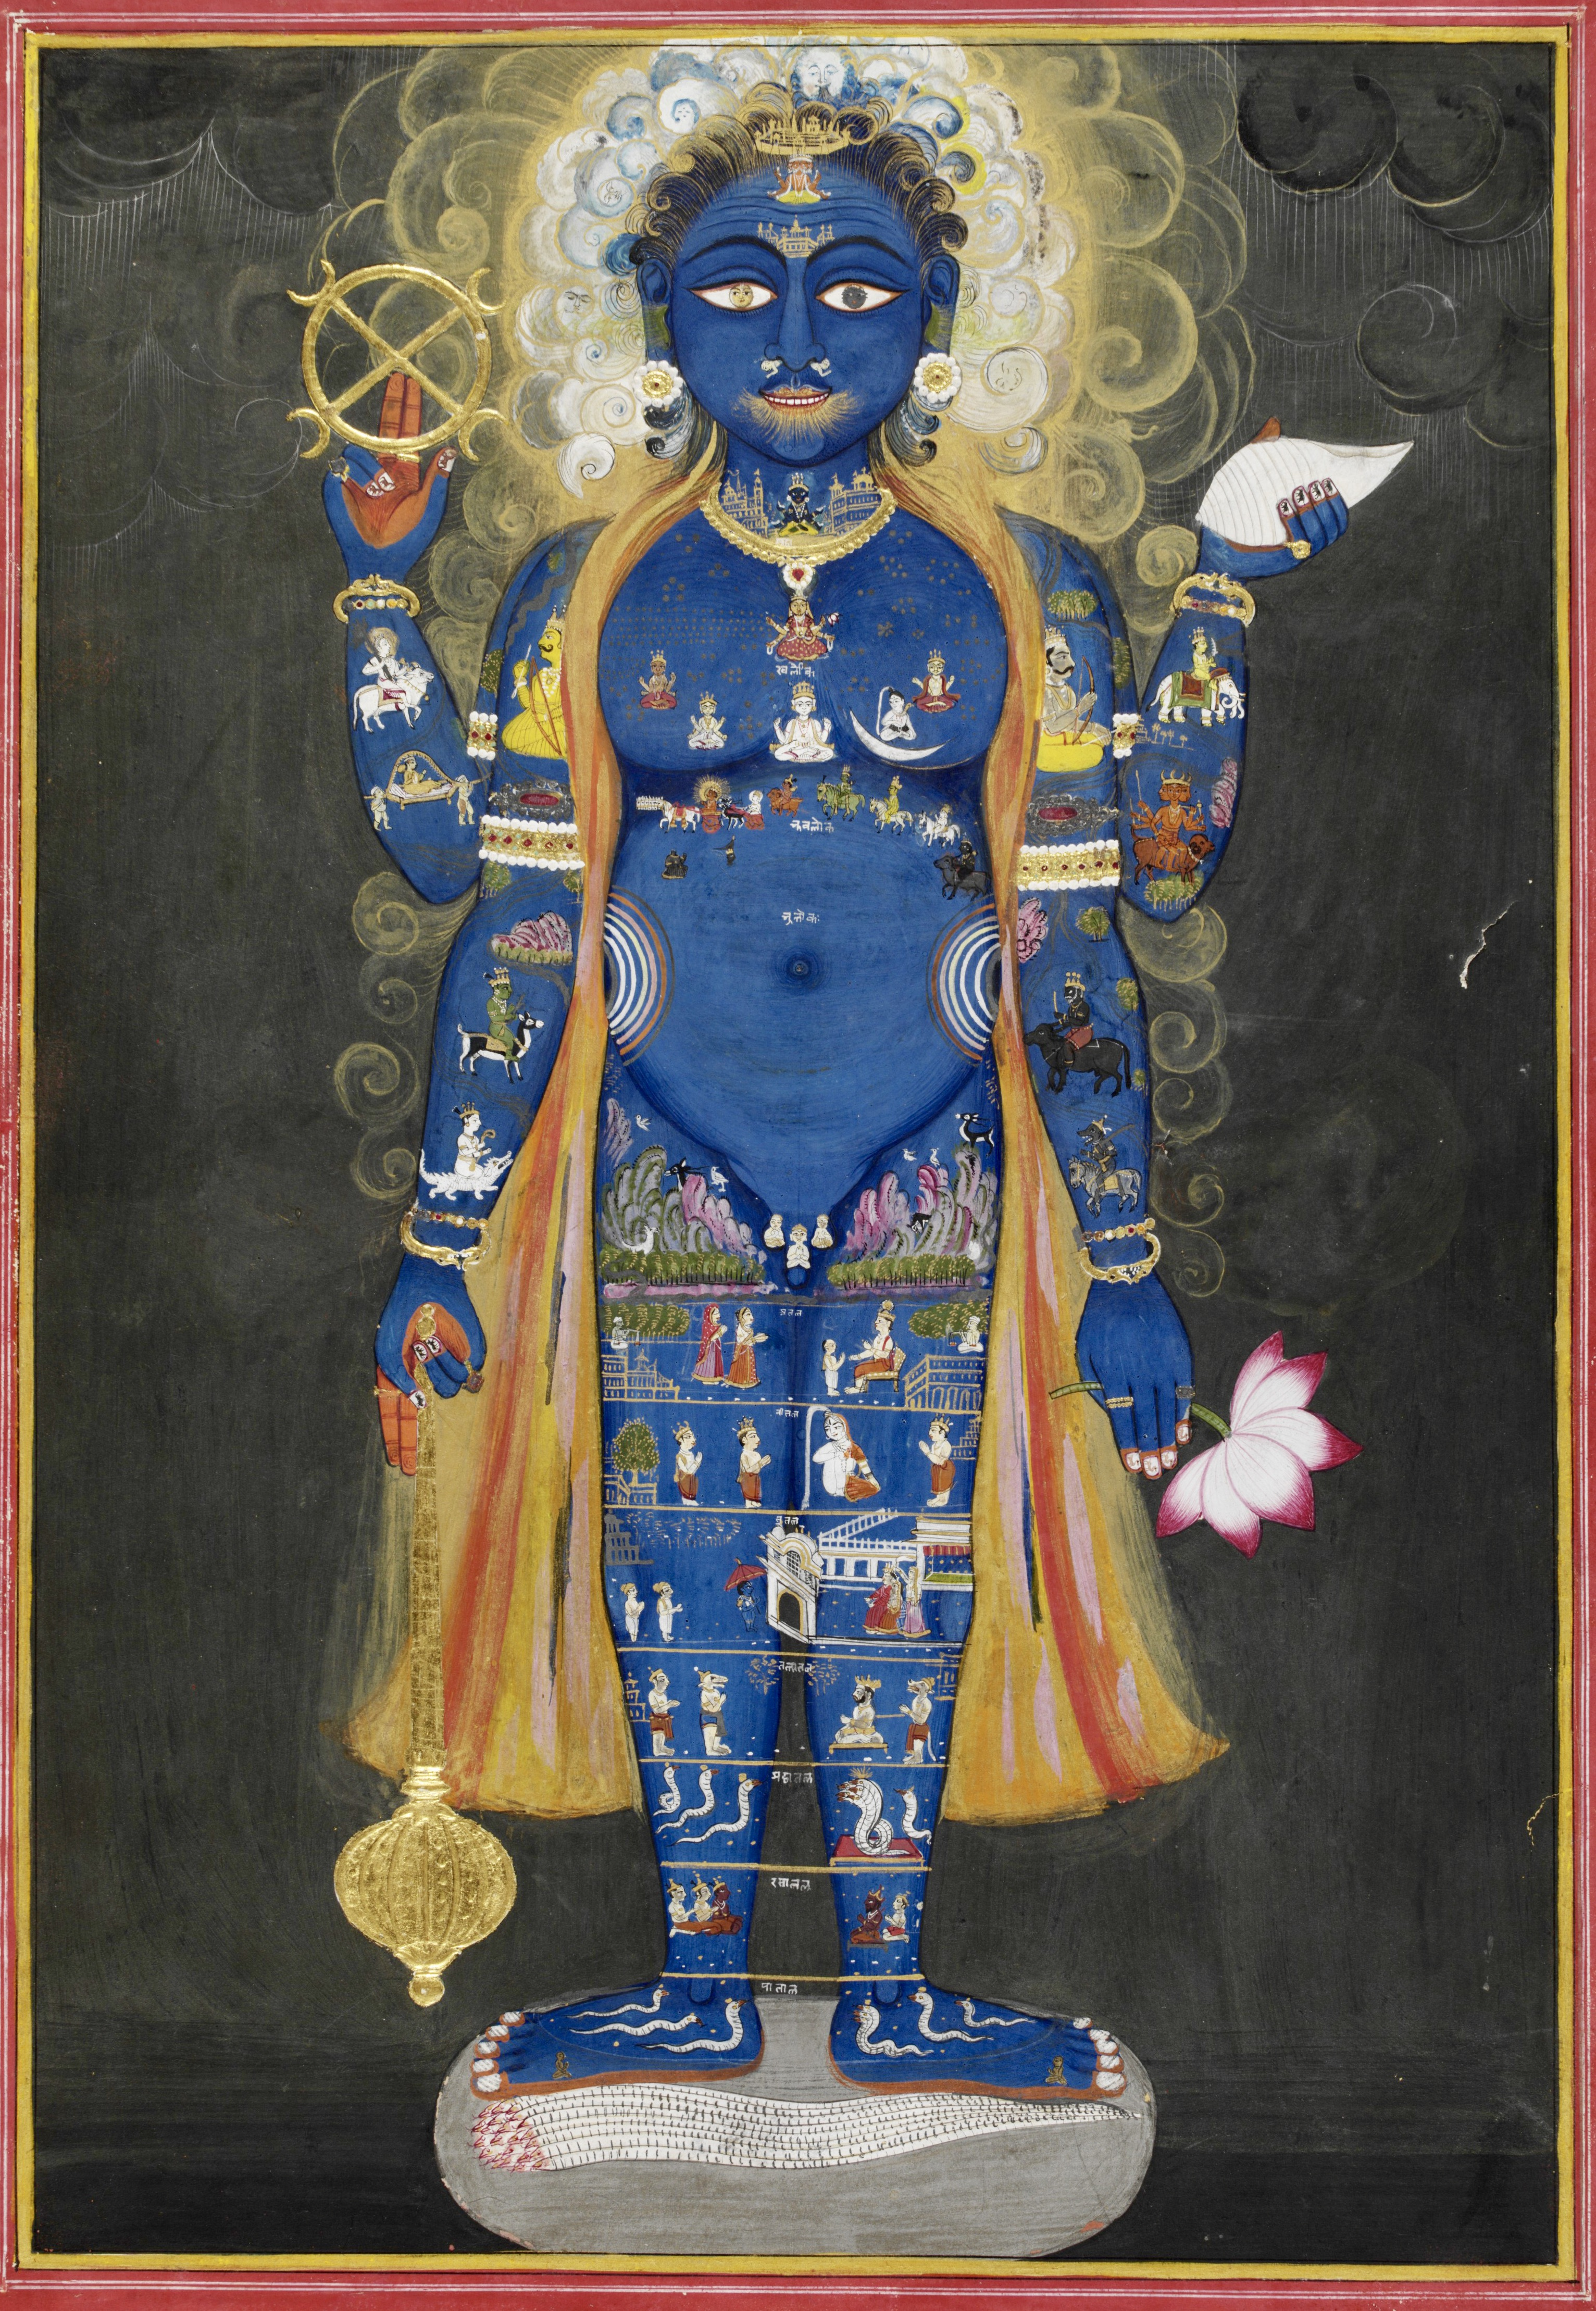
\includegraphics[width=1\textwidth]{pics/Vishnu_Vishvarupa_cropped.jpg}
	\caption{Viṣṇu Viśvarūpa, India, Rajasthan, Jaipur, ca. 1800–1820, Opaque watercolor and gold on paper, 38.5 × 28 cm, Victoria and Albert Museum, London, Given by Mrs. Gerald Clark.}
	\label{fig1}
      \end{figure}
\clearpage
  \begin{figure}[ht]
	\centering
  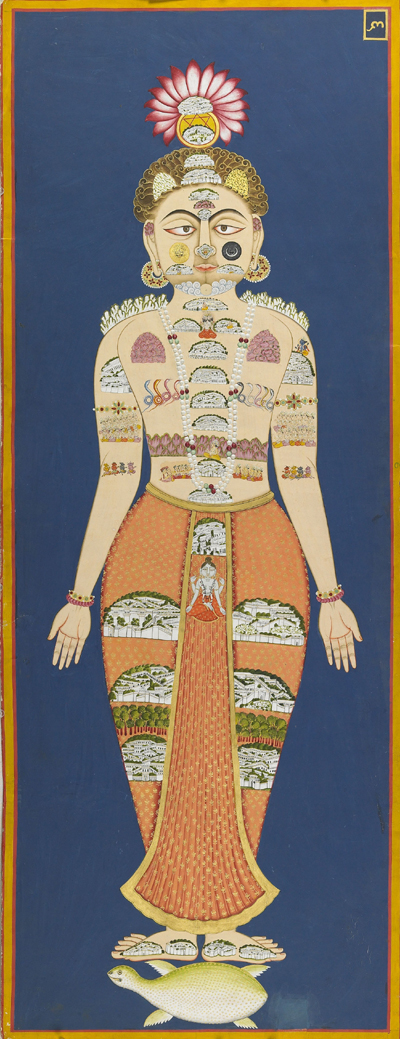
\includegraphics[width=0.5\textwidth]{pics/The_Equivalence_of_Self_and_Universe_(detail),_folio_6_from_the_Siddha_Siddhanta_Paddhati,_(Bulaki),_1824_(Samvat_1881);_122_x_46_cm._Mehrangarh_Museum_Trust..jpg}
	\caption{The Equivalence of Self and Universe (detail), folio 6 from the \textit{Siddhasiddhāntapaddhati} (Bulaki), India, Rajasthan, Jodhpur, 1824 (Samvat 1881), 122 x 46 cm, RJS 2378, Mehragarh Museum Trust.}
	\label{fig2}
      \end{figure}
      % \end{landscape}


\chapter{Bibliography}
 \label{sec:bibli}
   \clearpage
\newpage 
\thispagestyle{empty}
\quad  \addtocounter{page}{-1}

\printbibliography[heading=subbibintoc, title=Consulted Manuscripts, keyword=codex]

\printbibliography[heading=subbibintoc, title=Printed Editions, keyword=printsource]

\printbibliography[heading=subbibintoc, title=Secondary Literature, keyword=seclit]

\printbibliography[heading=subbibintoc, title=Online Sources, keyword=onlinesource]

\end{document}
